\documentclass{wissdoc}
% AutorInnen: Stefan Fliescher 2008, Anna Nelles 2010
% ----------------------------------------------------------------
% Diplomathesis
% ----------------------------------------------------------------
%%
%%
%%
% wissdoc Optionen: draft, relaxed, pdf --> siehe wissdoc.cls
% ------------------------------------------------------------------
% Weitere packages: (Dokumentation dazu durch "latex <package>.dtx")
%\usepackage{varioref}
%\usepackage{verbatim}
%\usepackage{float}    %z.B. \floatstyle{ruled}\restylefloat{figure}
\usepackage{subfigure}
%\usepackage{color}    % Farbiger/grauer Text
%\usepackage{colortbl}   % Farbige/graue Tabellenzeilen und -spalten!! <--
%\usepackage{fancybox} % fuer schattierte,ovale Boxen etc.
%\usepackage{tabularx} % automatische Spaltenbreite
%\usepackage{supertab} % mehrseitige Tabellen
%% -------------to find the position of bremsstrahlung photon candidates in--- end of usepackages -------------
\usepackage{latexsym}
\usepackage{amsfonts}
\usepackage{amsmath}
\usepackage{amssymb}
\usepackage{bm}
\usepackage{graphicx}
\usepackage{lscape}
\usepackage{url}
\usepackage{xspace}
\usepackage{listings}
\usepackage{floatflt}
\usepackage{sidecap}
%\usepackage{subfig}\captionsetup{labelfont=bf}
\usepackage[bf]{caption}%\captionsetup{captionlabel=it}
%\usepackage{subcaption}
\usepackage{xcolor}
\definecolor{cred1}{HTML}{CA0614}
\definecolor{cred2}{HTML}{FD3232}
%
%\def\Offline{\mbox{$\overline{\rm
%Off}$\hspace{.05em}\raisebox{.3ex}{$\underline{\rm line}$}}\xspace}
\def\OfflineB{\mbox{$\bf\overline{\rm\bf Off}$\hspace{.05em}
\raisebox{.2ex}{$\bf\underline{\rm\bf line}$}}\xspace}
\newcommand{\HRule}{\rule{\linewidth}{1mm}}

\def\emptyline{\vspace{12pt}}
%\renewcommand{\floatpagefraction}{.6}% vorher: .5
%\renewcommand{\textfraction}{.15} % vorher: .2
%% Informationen f�r die PDF-Datei
% \pdfinfo{
%  /Title  (Diplomathesis.pdf)
%  /Author (Stefan Fliescher)
%  /Subject (Diplomathesis)
%  /Keywords(Auger, Radio, Cosmic Rays)
% }

% Macros, nicht unbedingt notwendig
%%%%%%%%%%%%%%%%%%%%%%%%%%%%%%%%%%%%%%%%%%%%%%%%%%%%%%%%%%
% macros.tex -- einige mehr oder weniger nuetzliche Makros
% Autor: Roland Bless 1998
%%%%%%%%%%%%%%%%%%%%%%%%%%%%%%%%%%%%%%%%%%%%%%%%%%%%%%%%%%
% $Id: macros.tex,v 1.2 2001/01/24 20:13:04 bless Exp bless $
%%%%%%%%%%%%%%%%%%%%%%%%%%%%%%%%%%%%%%%%%%%%%%%%%%%%%%%%%%


%%%%%%%%%%%%%%%%%%%%%%%
% Kommentare 
%%%%%%%%%%%%%%%%%%%%%%%
\ifnotdraftelse{
\newcommand{\Kommentar}[1]{}
}{\newcommand{\Kommentar}[1]{{\em #1}}}
% Alles innerhalb von \Hide{} oder \ignore{} 
% wird von LaTeX komplett ignoriert (wie ein Kommentar)
\newcommand{\Hide}[1]{}
\let\ignore\Hide

%%%%%%%%%%%%%%%%%%%%%%%%%
% Leere Seite ohne Seitennummer, wird aber gezaehlt
%%%%%%%%%%%%%%%%%%%%%%%%%

\newcommand{\leereseite}{% Leerseite ohne Seitennummer, n�chste Seite rechts (wenn 2-seitig)
 \clearpage{\pagestyle{empty}\cleardoublepage}
}

%%%%%%%%%%%%%%%%%%%%%%%%%%
% Neue Seite rechts, leere linke Seite ohne Headings
%%%%%%%%%%%%%%%%%%%%%%%%%%
\newcommand{\xcleardoublepage}
{{\pagestyle{empty}\cleardoublepage}}

%%%%%%%%%%%%%%%%%%%%%%%%%%
% Tabellenspaltentypen (benoetigt colortbl)
%%%%%%%%%%%%%%%%%%%%%%%%%%
\newcommand{\PBS}[1]{\let\temp=\\#1\let\\=\temp}
\newcolumntype{y}{>{\PBS{\raggedright\hspace{0pt}}}p{1.35cm}}
\newcolumntype{z}{>{\PBS{\raggedright\hspace{0pt}}}p{2.5cm}}
\newcolumntype{q}{>{\PBS{\raggedright\hspace{0pt}}}p{6.5cm}}
\newcolumntype{g}{>{\columncolor[gray]{0.8}}c} % Grau
\newcolumntype{G}{>{\columncolor[gray]{0.9}}c} % helleres Grau

%%%%%%%%%%%%%%%%%%%%%%%%%%
% Anf�hrungszeichen oben und unten
%%%%%%%%%%%%%%%%%%%%%%%%%%
\newcommand{\anf}[1]{"`{#1}"'}

%%%%%%%%%%%%%%%%%%%%%%%%%%
% Tiefstellen von Text
%%%%%%%%%%%%%%%%%%%%%%%%%%
% S\tl{0} setzt die 0 unter das S (ohne Mathemodus!)
% zum Hochstellen gibt es uebrigens \textsuperscript
\makeatletter
\DeclareRobustCommand*\textlowerscript[1]{%
  \@textlowerscript{\selectfont#1}}
\def\@textlowerscript#1{%
  {\m@th\ensuremath{_{\mbox{\fontsize\sf@size\z@#1}}}}}
\let\tl\textlowerscript
\let\ts\textsuperscript
\makeatother

%%%%%%%%%%%%%%%%%%%%%%%%%%
% Gau�-Klammern
%%%%%%%%%%%%%%%%%%%%%%%%%%
\newcommand{\ceil}[1]{\lceil{#1}\rceil}
\newcommand{\floor}[1]{\lfloor{#1}\rfloor}

%%%%%%%%%%%%%%%%%%%%%%%%%%
% Average Operator (analog zu min, max)
%%%%%%%%%%%%%%%%%%%%%%%%%%
\def\avg{\mathop{\mathgroup\symoperators avg}}

%%%%%%%%%%%%%%%%%%%%%%%%%%
% Wortabk�rzungen
%%%%%%%%%%%%%%%%%%%%%%%%%%
\def\zB{z.\,B.\ }
\def\dh{d.\,h.\ }
\def\ua{u.\,a.\ }
\def\su{s.\,u.\ }
\newcommand{\bzw}{bzw.\ }

%%%%%%%%%%%%%%%%%%%%%%%%%%%%%%%%%%%
% Einbinden von Graphiken
%%%%%%%%%%%%%%%%%%%%%%%%%%%%%%%%%%%
% global scaling factor
\def\gsf{0.9}
%% Graphik, 
%% 3 Argumente: Datei, Label, Unterschrift
\newcommand{\Abbildung}[3]{%
\begin{figure}[tbh] %
\centerline{\scalebox{\gsf}{\includegraphics*{#1}}} %
\caption{#3} %
\label{#2} %
\end{figure} %
}
\let\Abb\Abbildung
%% Abbps
%% Graphik, skaliert, Angabe der Position
%% 5 Argumente: Position, Breite (0 bis 1.0), Datei, Label, Unterschrift
\newcommand{\Abbildungps}[5]{%
\begin{figure}[#1]%
\begin{center}
\scalebox{\gsf}{\includegraphics*[width=#2\textwidth]{#3}}%
\caption{#5}%
\label{#4}%
\end{center}
\end{figure}%
}
\let\Abbps\Abbildungps
%% Graphik, Angabe der Position, frei w�hlbares Argument f�r includegraphics
%% 5 Argumente: Position, Optionen, Datei, Label, Unterschrift
\newcommand{\Abbildungpf}[5]{%
\begin{figure}[#1]%
\begin{center}
\scalebox{\gsf}{\includegraphics*[#2]{#3}}%
\caption{#5}%
\label{#4}%
\end{center}
\end{figure}%
}
\let\Abbpf\Abbildungpf

%%
% Anmerkung: \resizebox{x}{y}{box} skaliert die box auf Breite x und H�he y,
%            ist x oder y ein !, dann wird das uspr�ngliche 
%            Seitenverh�ltnis beibehalten.
%            \rescalebox funktioniert �hnlich, nur das dort ein Faktor
%            statt einer Dimension angegeben wird.
%%
% \Abbps{Position}{Breite in Bruchteilen der Textbreite}{Dateiname}{Label}{Bildunterschrift}
%

\newcommand{\refAbb}[1]{%
s.~Abbildung \ref{#1}}

%%%%%%%%%%%%%%%%%%%%
%% end of macros.tex
%%%%%%%%%%%%%%%%%%%%
% %%%%%%%%%%%%%%%%%%%%
%  for LHCb aliases
% %%%%%%%%%%%%%%%%%%%%
\usepackage{ifthen}
\newboolean{articletitles}
\setboolean{articletitles}{true} % False removes titles in references
\newboolean{uprightparticles}
\setboolean{uprightparticles}{false} %Set to true to get roman particle symbols
\usepackage{amssymb}
\usepackage{amsfonts}
\usepackage{paralist}
\usepackage{wrapfig}
\usepackage{upgreek} % Adds in support for greek letters in roman typeset
% Get hyperlinks to captions and in references.
% These do not work with revtex. Use "hypertext" as class option instead.
\usepackage{hyperref}    % Hyperlinks in references
\usepackage[all]{hypcap} % Internal hyperlinks to floats.
%%% $Id: lhcb-symbols-def.tex 16562 2012-03-01 08:41:50Z uegede $
%%% ======================================================================
%%% Purpose: standard LHCb aliases
%%% Author: Originally Ulrik Egede, adapted by Tomasz Skwarnicki for templates,
%%% rewritten by Chris Parkes
%%% Created on: 2009-09-24
%%% =======================================================================

%%% this has to go before \begin{document}
%%%\usepackage{ifthen} 
%%%\newboolean{uprightparticles}
%%%\setboolean{uprightparticles}{true} %Set to false to get italic particle symbols

%%% Add comments with at least three %%% preceding.
%%% Add new sections with one % preceding
%%% Add new subsections with two %% preceding

%%%%%%%%%%%%%
% Experiments
%%%%%%%%%%%%%
\def\lhcb {LHCb\xspace}
\def\lal {LAL\xspace}
\def\ux85 {UX85\xspace}
\def\cern {CERN\xspace}
\def\lhc {LHC\xspace}
\def\atlas {ATLAS\xspace}
\def\cms {CMS\xspace}
\def\babar  {BaBar\xspace}
\def\belle  {Belle\xspace}
\def\aleph  {ALEPH\xspace}
\def\delphi {DELPHI\xspace}
\def\opal   {OPAL\xspace}
\def\lthree {L3\xspace}
\def\lep    {LEP\xspace}
\def\cdf    {CDF\xspace}
\def\dzero  {D\O\xspace}
\def\sld    {SLD\xspace}
\def\cleo   {CLEO\xspace}
\def\uaone  {UA1\xspace}
\def\uatwo  {UA2\xspace}
\def\tevatron {TEVATRON\xspace}

%% LHCb sub-detectors and sub-systems

\def\pu     {PU\xspace}
\def\velo   {VELO\xspace}
\def\rich   {RICH\xspace}
\def\richone {RICH1\xspace}
\def\richtwo {RICH2\xspace}
\def\ttracker {TT\xspace}
\def\intr   {IT\xspace}
\def\st     {ST\xspace}
\def\ot     {OT\xspace}
\def\Tone   {T1\xspace}
\def\Ttwo   {T2\xspace}
\def\Tthree {T3\xspace}
\def\Mone   {M1\xspace}
\def\Mtwo   {M2\xspace}
\def\Mthree {M3\xspace}
\def\Mfour  {M4\xspace}
\def\Mfive  {M5\xspace}
\def\ecal   {ECAL\xspace}
\def\spd    {SPD\xspace}
\def\presh  {PS\xspace}
\def\hcal   {HCAL\xspace}
\def\bcm    {BCM\xspace}

\def\ode    {ODE\xspace}
\def\daq    {DAQ\xspace}
\def\tfc    {TFC\xspace}
\def\ecs    {ECS\xspace}
\def\lone   {L0\xspace}
\def\hlt    {HLT\xspace}
\def\hltone {HLT1\xspace}
\def\hlttwo {HLT2\xspace}

%%% Upright (not slanted) Particles

\ifthenelse{\boolean{uprightparticles}}%
{\def\Palpha      {\ensuremath{\upalpha}\xspace}
 \def\Pbeta       {\ensuremath{\upbeta}\xspace}
 \def\Pgamma      {\ensuremath{\upgamma}\xspace}                 
 \def\Pdelta      {\ensuremath{\updelta}\xspace}                 
 \def\Pepsilon    {\ensuremath{\upepsilon}\xspace}                 
 \def\Pvarepsilon {\ensuremath{\upvarepsilon}\xspace}                 
 \def\Pzeta       {\ensuremath{\upzeta}\xspace}                 
 \def\Peta        {\ensuremath{\upeta}\xspace}                 
 \def\Ptheta      {\ensuremath{\uptheta}\xspace}                 
 \def\Pvartheta   {\ensuremath{\upvartheta}\xspace}                 
 \def\Piota       {\ensuremath{\upiota}\xspace}                 
 \def\Pkappa      {\ensuremath{\upkappa}\xspace}                 
 \def\Plambda     {\ensuremath{\uplambda}\xspace}                 
 \def\Pmu         {\ensuremath{\upmu}\xspace}                 
 \def\Pnu         {\ensuremath{\upnu}\xspace}                 
 \def\Pxi         {\ensuremath{\upxi}\xspace}                 
 \def\Ppi         {\ensuremath{\uppi}\xspace}                 
 \def\Pvarpi      {\ensuremath{\upvarpi}\xspace}                 
 \def\Prho        {\ensuremath{\uprho}\xspace}                 
 \def\Pvarrho     {\ensuremath{\upvarrho}\xspace}                 
 \def\Ptau        {\ensuremath{\uptau}\xspace}                 
 \def\Pupsilon    {\ensuremath{\upupsilon}\xspace}                 
 \def\Pphi        {\ensuremath{\upphi}\xspace}                 
 \def\Pvarphi     {\ensuremath{\upvarphi}\xspace}                 
 \def\Pchi        {\ensuremath{\upchi}\xspace}                 
 \def\Ppsi        {\ensuremath{\uppsi}\xspace}                 
 \def\Pomega      {\ensuremath{\upomega}\xspace}                 

 \def\PDelta      {\ensuremath{\Delta}\xspace}                 
 \def\PXi      {\ensuremath{\Xi}\xspace}                 
 \def\PLambda      {\ensuremath{\Lambda}\xspace}                 
 \def\PSigma      {\ensuremath{\Sigma}\xspace}                 
 \def\POmega      {\ensuremath{\Omega}\xspace}                 
 \def\PUpsilon      {\ensuremath{\Upsilon}\xspace}                 
 
 %\mathchardef\Deltares="7101
 %\mathchardef\Xi="7104
 %\mathchardef\Lambda="7103
 %\mathchardef\Sigma="7106
 %\mathchardef\Omega="710A


 \def\PA      {\ensuremath{\mathrm{A}}\xspace}                 
 \def\PB      {\ensuremath{\mathrm{B}}\xspace}                 
 \def\PC      {\ensuremath{\mathrm{C}}\xspace}                 
 \def\PD      {\ensuremath{\mathrm{D}}\xspace}                 
 \def\PE      {\ensuremath{\mathrm{E}}\xspace}                 
 \def\PF      {\ensuremath{\mathrm{F}}\xspace}                 
 \def\PG      {\ensuremath{\mathrm{G}}\xspace}                 
 \def\PH      {\ensuremath{\mathrm{H}}\xspace}                 
 \def\PI      {\ensuremath{\mathrm{I}}\xspace}                 
 \def\PJ      {\ensuremath{\mathrm{J}}\xspace}                 
 \def\PK      {\ensuremath{\mathrm{K}}\xspace}                 
 \def\PL      {\ensuremath{\mathrm{L}}\xspace}                 
 \def\PM      {\ensuremath{\mathrm{M}}\xspace}                 
 \def\PN      {\ensuremath{\mathrm{N}}\xspace}                 
 \def\PO      {\ensuremath{\mathrm{O}}\xspace}                 
 \def\PP      {\ensuremath{\mathrm{P}}\xspace}                 
 \def\PQ      {\ensuremath{\mathrm{Q}}\xspace}                 
 \def\PR      {\ensuremath{\mathrm{R}}\xspace}                 
 \def\PS      {\ensuremath{\mathrm{S}}\xspace}                 
 \def\PT      {\ensuremath{\mathrm{T}}\xspace}                 
 \def\PU      {\ensuremath{\mathrm{U}}\xspace}                 
 \def\PV      {\ensuremath{\mathrm{V}}\xspace}                 
 \def\PW      {\ensuremath{\mathrm{W}}\xspace}                 
 \def\PX      {\ensuremath{\mathrm{X}}\xspace}                 
 \def\PY      {\ensuremath{\mathrm{Y}}\xspace}                 
 \def\PZ      {\ensuremath{\mathrm{Z}}\xspace}                 
 \def\Pa      {\ensuremath{\mathrm{a}}\xspace}                 
 \def\Pb      {\ensuremath{\mathrm{b}}\xspace}                 
 \def\Pc      {\ensuremath{\mathrm{c}}\xspace}                 
 \def\Pd      {\ensuremath{\mathrm{d}}\xspace}                 
 \def\Pe      {\ensuremath{\mathrm{e}}\xspace}                 
 \def\Pf      {\ensuremath{\mathrm{f}}\xspace}                 
 \def\Pg      {\ensuremath{\mathrm{g}}\xspace}                 
 \def\Ph      {\ensuremath{\mathrm{h}}\xspace}                 
 \def\Pi      {\ensuremath{\mathrm{i}}\xspace}                 
 \def\Pj      {\ensuremath{\mathrm{j}}\xspace}                 
 \def\Pk      {\ensuremath{\mathrm{k}}\xspace}                 
 \def\Pl      {\ensuremath{\mathrm{l}}\xspace}                 
 \def\Pm      {\ensuremath{\mathrm{m}}\xspace}                 
 \def\Pn      {\ensuremath{\mathrm{n}}\xspace}                 
 \def\Po      {\ensuremath{\mathrm{o}}\xspace}                 
 \def\Pp      {\ensuremath{\mathrm{p}}\xspace}                 
 \def\Pq      {\ensuremath{\mathrm{q}}\xspace}                 
 \def\Pr      {\ensuremath{\mathrm{r}}\xspace}                 
 \def\Ps      {\ensuremath{\mathrm{s}}\xspace}                 
 \def\Pt      {\ensuremath{\mathrm{t}}\xspace}                 
 \def\Pu      {\ensuremath{\mathrm{u}}\xspace}                 
 \def\Pv      {\ensuremath{\mathrm{v}}\xspace}                 
 \def\Pw      {\ensuremath{\mathrm{w}}\xspace}                 
 \def\Px      {\ensuremath{\mathrm{x}}\xspace}                 
 \def\Py      {\ensuremath{\mathrm{y}}\xspace}                 
 \def\Pz      {\ensuremath{\mathrm{z}}\xspace}                 
}
{\def\Palpha      {\ensuremath{\alpha}\xspace}
 \def\Pbeta       {\ensuremath{\beta}\xspace}
 \def\Pgamma      {\ensuremath{\gamma}\xspace}                 
 \def\Pdelta      {\ensuremath{\delta}\xspace}                 
 \def\Pepsilon    {\ensuremath{\epsilon}\xspace}                 
 \def\Pvarepsilon {\ensuremath{\varepsilon}\xspace}                 
 \def\Pzeta       {\ensuremath{\zeta}\xspace}                 
 \def\Peta        {\ensuremath{\eta}\xspace}                 
 \def\Ptheta      {\ensuremath{\theta}\xspace}                 
 \def\Pvartheta   {\ensuremath{\vartheta}\xspace}                 
 \def\Piota       {\ensuremath{\iota}\xspace}                 
 \def\Pkappa      {\ensuremath{\kappa}\xspace}                 
 \def\Plambda     {\ensuremath{\lambda}\xspace}                 
 \def\Pmu         {\ensuremath{\mu}\xspace}                 
 \def\Pnu         {\ensuremath{\nu}\xspace}                 
 \def\Pxi         {\ensuremath{\xi}\xspace}                 
 \def\Ppi         {\ensuremath{\pi}\xspace}                 
 \def\Pvarpi      {\ensuremath{\varpi}\xspace}                 
 \def\Prho        {\ensuremath{\rho}\xspace}                 
 \def\Pvarrho     {\ensuremath{\varrho}\xspace}                 
 \def\Ptau        {\ensuremath{\tau}\xspace}                 
 \def\Pupsilon    {\ensuremath{\upsilon}\xspace}                 
 \def\Pphi        {\ensuremath{\phi}\xspace}                 
 \def\Pvarphi     {\ensuremath{\varphi}\xspace}                 
 \def\Pchi        {\ensuremath{\chi}\xspace}                 
 \def\Ppsi        {\ensuremath{\psi}\xspace}                 
 \def\Pomega      {\ensuremath{\omega}\xspace}                 
 \mathchardef\PDelta="7101
 \mathchardef\PXi="7104
 \mathchardef\PLambda="7103
 \mathchardef\PSigma="7106
 \mathchardef\POmega="710A
 \mathchardef\PUpsilon="7107
 \def\PA      {\ensuremath{A}\xspace}                 
 \def\PB      {\ensuremath{B}\xspace}                 
 \def\PC      {\ensuremath{C}\xspace}                 
 \def\PD      {\ensuremath{D}\xspace}                 
 \def\PE      {\ensuremath{E}\xspace}                 
 \def\PF      {\ensuremath{F}\xspace}                 
 \def\PG      {\ensuremath{G}\xspace}                 
 \def\PH      {\ensuremath{H}\xspace}                 
 \def\PI      {\ensuremath{I}\xspace}                 
 \def\PJ      {\ensuremath{J}\xspace}                 
 \def\PK      {\ensuremath{K}\xspace}                 
 \def\PL      {\ensuremath{L}\xspace}                 
 \def\PM      {\ensuremath{M}\xspace}                 
 \def\PN      {\ensuremath{N}\xspace}                 
 \def\PO      {\ensuremath{O}\xspace}                 
 \def\PP      {\ensuremath{P}\xspace}                 
 \def\PQ      {\ensuremath{Q}\xspace}                 
 \def\PR      {\ensuremath{R}\xspace}                 
 \def\PS      {\ensuremath{S}\xspace}                 
 \def\PT      {\ensuremath{T}\xspace}                 
 \def\PU      {\ensuremath{U}\xspace}                 
 \def\PV      {\ensuremath{V}\xspace}                 
 \def\PW      {\ensuremath{W}\xspace}                 
 \def\PX      {\ensuremath{X}\xspace}                 
 \def\PY      {\ensuremath{Y}\xspace}                 
 \def\PZ      {\ensuremath{Z}\xspace}                 
 \def\Pa      {\ensuremath{a}\xspace}                 
 \def\Pb      {\ensuremath{b}\xspace}                 
 \def\Pc      {\ensuremath{c}\xspace}                 
 \def\Pd      {\ensuremath{d}\xspace}                 
 \def\Pe      {\ensuremath{e}\xspace}                 
 \def\Pf      {\ensuremath{f}\xspace}                 
 \def\Pg      {\ensuremath{g}\xspace}                 
 \def\Ph      {\ensuremath{h}\xspace}                 
 \def\Pi      {\ensuremath{i}\xspace}                 
 \def\Pj      {\ensuremath{j}\xspace}                 
 \def\Pk      {\ensuremath{k}\xspace}                 
 \def\Pl      {\ensuremath{l}\xspace}                 
 \def\Pm      {\ensuremath{m}\xspace}                 
 \def\Pn      {\ensuremath{n}\xspace}                 
 \def\Po      {\ensuremath{o}\xspace}                 
 \def\Pp      {\ensuremath{p}\xspace}                 
 \def\Pq      {\ensuremath{q}\xspace}                 
 \def\Pr      {\ensuremath{r}\xspace}                 
 \def\Ps      {\ensuremath{s}\xspace}                 
 \def\Pt      {\ensuremath{t}\xspace}                 
 \def\Pu      {\ensuremath{u}\xspace}                 
 \def\Pv      {\ensuremath{v}\xspace}                 
 \def\Pw      {\ensuremath{w}\xspace}                 
 \def\Px      {\ensuremath{x}\xspace}                 
 \def\Py      {\ensuremath{y}\xspace}                 
 \def\Pz      {\ensuremath{z}\xspace}                 
}

%%%%%%%%%%%%%%%%%%%%%%%%%%%%%%%%%%%%%%%%%%%%%%%
%My decays 
\def\BToDK      {\decay{\Bpm}{\Dz\Kpm}}
\def\BToD4PiK      {\decay{\Bpm}{{\decay{\Dz}{4 \pion}}\Kpm}}
\def\DzTo4Pi		{\decay{\Dz}{4\pion}}
\def\DTo4Pi		{\decay{\D}{4\pion}}
\def\4Pi        {4\pion}
\def\KsPiPi     {{\KS}{\pion}\pion}
\def\KlPiPi		{{\KL}{\pion}\pion}
\def\KtPi		{{\kaon}3\pion}
\def\KsKs	{{\KS}{\KS}}


% Particles

%% leptons


\let\emi\en
\def\electron   {\ensuremath{\Pe}\xspace}
\def\en         {\ensuremath{\Pe^-}\xspace}   % electron negative (\em is taken)
\def\ep         {\ensuremath{\Pe^+}\xspace}
\def\epm        {\ensuremath{\Pe^\pm}\xspace} 
\def\epem       {\ensuremath{\Pe^+\Pe^-}\xspace}
\def\ee         {\ensuremath{\Pe^-\Pe^-}\xspace}

\def\mmu        {\ensuremath{\Pmu}\xspace}
\def\mup        {\ensuremath{\Pmu^+}\xspace}
\def\mun        {\ensuremath{\Pmu^-}\xspace} % muon negative (\mum is taken)
\def\mumu       {\ensuremath{\Pmu^+\Pmu^-}\xspace}
\def\mtau       {\ensuremath{\Ptau}\xspace}

\def\taup       {\ensuremath{\Ptau^+}\xspace}
\def\taum       {\ensuremath{\Ptau^-}\xspace}
\def\tautau     {\ensuremath{\Ptau^+\Ptau^-}\xspace}

\def\ellm       {\ensuremath{\ell^-}\xspace}
\def\ellp       {\ensuremath{\ell^+}\xspace}
\def\ellell     {\ensuremath{\ell^+ \ell^-}\xspace}

\def\neu        {\ensuremath{\Pnu}\xspace}
\def\neub       {\ensuremath{\overline{\Pnu}}\xspace}
\def\nuenueb    {\ensuremath{\neu\neub}\xspace}
\def\neue       {\ensuremath{\neu_e}\xspace}
\def\neueb      {\ensuremath{\neub_e}\xspace}
\def\neueneueb  {\ensuremath{\neue\neueb}\xspace}
\def\neum       {\ensuremath{\neu_\mu}\xspace}
\def\neumb      {\ensuremath{\neub_\mu}\xspace}
\def\neumneumb  {\ensuremath{\neum\neumb}\xspace}
\def\neut       {\ensuremath{\neu_\tau}\xspace}
\def\neutb      {\ensuremath{\neub_\tau}\xspace}
\def\neutneutb  {\ensuremath{\neut\neutb}\xspace}
\def\neul       {\ensuremath{\neu_\ell}\xspace}
\def\neulb      {\ensuremath{\neub_\ell}\xspace}
\def\neulneulb  {\ensuremath{\neul\neulb}\xspace}

%% Gauge bosons and scalars

\def\g      {\ensuremath{\Pgamma}\xspace}
\def\H      {\ensuremath{\PH^0}\xspace}
\def\Hp     {\ensuremath{\PH^+}\xspace}
\def\Hm     {\ensuremath{\PH^-}\xspace}
\def\Hpm    {\ensuremath{\PH^\pm}\xspace}
\def\W      {\ensuremath{\PW}\xspace}
\def\Wp     {\ensuremath{\PW^+}\xspace}
\def\Wm     {\ensuremath{\PW^-}\xspace}
\def\Wpm    {\ensuremath{\PW^\pm}\xspace}
\def\Z      {\ensuremath{\PZ^0}\xspace}

%% Quarks

\def\quark     {\ensuremath{\Pq}\xspace}
\def\quarkbar  {\ensuremath{\overline \quark}\xspace}
\def\qqbar     {\ensuremath{\quark\quarkbar}\xspace}
\def\uquark    {\ensuremath{\Pu}\xspace}
\def\uquarkbar {\ensuremath{\overline \uquark}\xspace}
\def\uubar     {\ensuremath{\uquark\uquarkbar}\xspace}
\def\dquark    {\ensuremath{\Pd}\xspace}
\def\dquarkbar {\ensuremath{\overline \dquark}\xspace}
\def\ddbar     {\ensuremath{\dquark\dquarkbar}\xspace}
\def\squark    {\ensuremath{\Ps}\xspace}
\def\squarkbar {\ensuremath{\overline \squark}\xspace}
\def\ssbar     {\ensuremath{\squark\squarkbar}\xspace}
\def\cquark    {\ensuremath{\Pc}\xspace}
\def\cquarkbar {\ensuremath{\overline \cquark}\xspace}
\def\ccbar     {\ensuremath{\cquark\cquarkbar}\xspace}
\def\bquark    {\ensuremath{\Pb}\xspace}
\def\bquarkbar {\ensuremath{\overline \bquark}\xspace}
\def\bbbar     {\ensuremath{\bquark\bquarkbar}\xspace}
\def\tquark    {\ensuremath{\Pt}\xspace}
\def\tquarkbar {\ensuremath{\overline \tquark}\xspace}
\def\ttbar     {\ensuremath{\tquark\tquarkbar}\xspace}

%% Light mesons

\def\pion  {\ensuremath{\Ppi}\xspace}
\def\piz   {\ensuremath{\pion^0}\xspace}
\def\pizs  {\ensuremath{\pion^0\mbox\,\rm{s}}\xspace}
\def\ppz   {\ensuremath{\pion^0\pion^0}\xspace}
\def\pip   {\ensuremath{\pion^+}\xspace}
\def\pim   {\ensuremath{\pion^-}\xspace}
\def\pipi  {\ensuremath{\pion^+\pion^-}\xspace}
\def\pipm  {\ensuremath{\pion^\pm}\xspace}
\def\pimp  {\ensuremath{\pion^\mp}\xspace}

\def\kaon  {\ensuremath{\PK}\xspace}
%%% do NOT use ensuremath here
  \def\Kbar  {\kern 0.2em\overline{\kern -0.2em \PK}{}\xspace}
\def\Kb    {\ensuremath{\Kbar}\xspace}
\def\Kz    {\ensuremath{\kaon^0}\xspace}
\def\Kzb   {\ensuremath{\Kbar^0}\xspace}
\def\KzKzb {\ensuremath{\Kz \kern -0.16em \Kzb}\xspace}
\def\Kp    {\ensuremath{\kaon^+}\xspace}
\def\Km    {\ensuremath{\kaon^-}\xspace}
\def\Kpm   {\ensuremath{\kaon^\pm}\xspace}
\def\Kmp   {\ensuremath{\kaon^\mp}\xspace}
\def\KpKm  {\ensuremath{\Kp \kern -0.16em \Km}\xspace}
\def\KS    {\ensuremath{\kaon^0_{\rm\scriptscriptstyle S}}\xspace} 
\def\KL    {\ensuremath{\kaon^0_{\rm\scriptscriptstyle L}}\xspace} 
\def\Kstarz  {\ensuremath{\kaon^{*0}}\xspace}
\def\Kstarzb {\ensuremath{\Kbar^{*0}}\xspace}
\def\Kstar   {\ensuremath{\kaon^*}\xspace}
\def\Kstarb  {\ensuremath{\Kbar^*}\xspace}
\def\Kstarp  {\ensuremath{\kaon^{*+}}\xspace}
\def\Kstarm  {\ensuremath{\kaon^{*-}}\xspace}
\def\Kstarpm {\ensuremath{\kaon^{*\pm}}\xspace}
\def\Kstarmp {\ensuremath{\kaon^{*\mp}}\xspace}

\newcommand{\etapr}{\ensuremath{\Peta^{\prime}}\xspace}

%% Heavy mesons

%%% do NOT use ensuremath here
  \def\Dbar    {\kern 0.2em\overline{\kern -0.2em \PD}{}\xspace}
\def\D       {\ensuremath{\PD}\xspace}
\def\Db      {\ensuremath{\Dbar}\xspace}
\def\Dz      {\ensuremath{\D^0}\xspace}
\def\Dzb     {\ensuremath{\Dbar^0}\xspace}
\def\DzDzb   {\ensuremath{\Dz {\kern -0.16em \Dzb}}\xspace}
\def\Dp      {\ensuremath{\D^+}\xspace}
\def\Dm      {\ensuremath{\D^-}\xspace}
\def\Dpm     {\ensuremath{\D^\pm}\xspace}
\def\Dmp     {\ensuremath{\D^\mp}\xspace}
\def\DpDm    {\ensuremath{\Dp {\kern -0.16em \Dm}}\xspace}
\def\Dstar   {\ensuremath{\D^*}\xspace}
\def\Dstarb  {\ensuremath{\Dbar^*}\xspace}
\def\Dstarz  {\ensuremath{\D^{*0}}\xspace}
\def\Dstarzb {\ensuremath{\Dbar^{*0}}\xspace}
\def\Dstarp  {\ensuremath{\D^{*+}}\xspace}
\def\Dstarm  {\ensuremath{\D^{*-}}\xspace}
\def\Dstarpm {\ensuremath{\D^{*\pm}}\xspace}
\def\Dstarmp {\ensuremath{\D^{*\mp}}\xspace}
\def\Ds      {\ensuremath{\D^+_\squark}\xspace}
\def\Dsp     {\ensuremath{\D^+_\squark}\xspace}
\def\Dsm     {\ensuremath{\D^-_\squark}\xspace}
\def\Dspm    {\ensuremath{\D^{\pm}_\squark}\xspace}
\def\Dss     {\ensuremath{\D^{*+}_\squark}\xspace}
\def\Dssp    {\ensuremath{\D^{*+}_\squark}\xspace}
\def\Dssm    {\ensuremath{\D^{*-}_\squark}\xspace}
\def\Dsspm   {\ensuremath{\D^{*\pm}_\squark}\xspace}

\def\B       {\ensuremath{\PB}\xspace}
%%% do NOT use ensuremath here
  \def\Bbar    {\kern 0.18em\overline{\kern -0.18em \PB}{}\xspace}
\def\Bb      {\ensuremath{\Bbar}\xspace}
\def\BBbar   {\ensuremath{\B\Bbar}\xspace} 
\def\Bz      {\ensuremath{\B^0}\xspace}
\def\Bzb     {\ensuremath{\Bbar^0}\xspace}
\def\Bu      {\ensuremath{\B^+}\xspace}
\def\Bub     {\ensuremath{\B^-}\xspace}
\def\Bp      {\ensuremath{\Bu}\xspace}
\def\Bm      {\ensuremath{\Bub}\xspace}
\def\Bpm     {\ensuremath{\B^\pm}\xspace}
\def\Bmp     {\ensuremath{\B^\mp}\xspace}
\def\Bd      {\ensuremath{\B^0}\xspace}
\def\Bs      {\ensuremath{\B^0_\squark}\xspace}
\def\Bsb     {\ensuremath{\Bbar^0_\squark}\xspace}
\def\Bdb     {\ensuremath{\Bbar^0}\xspace}
\def\Bc      {\ensuremath{\B_\cquark^+}\xspace}
\def\Bcp     {\ensuremath{\B_\cquark^+}\xspace}
\def\Bcm     {\ensuremath{\B_\cquark^-}\xspace}
\def\Bcpm    {\ensuremath{\B_\cquark^\pm}\xspace}

%% Onia

\def\jpsi     {\ensuremath{{\PJ\mskip -3mu/\mskip -2mu\Ppsi\mskip 2mu}}\xspace}
\def\psitwos  {\ensuremath{\Ppsi{(2S)}}\xspace}
\def\psiprpr  {\ensuremath{\Ppsi(3770)}\xspace}
\def\etac     {\ensuremath{\Peta_\cquark}\xspace}
\def\chiczero {\ensuremath{\Pchi_{\cquark 0}}\xspace}
\def\chicone  {\ensuremath{\Pchi_{\cquark 1}}\xspace}
\def\chictwo  {\ensuremath{\Pchi_{\cquark 2}}\xspace}
  %\mathchardef\Upsilon="7107
  \def\Y#1S{\ensuremath{\PUpsilon{(#1S)}}\xspace}% no space before {...}!
\def\OneS  {\Y1S}
\def\TwoS  {\Y2S}
\def\ThreeS{\Y3S}
\def\FourS {\Y4S}
\def\FiveS {\Y5S}

\def\chic  {\ensuremath{\Pchi_{c}}\xspace}

%% Baryons

\def\proton      {\ensuremath{\Pp}\xspace}
\def\antiproton  {\ensuremath{\overline \proton}\xspace}
\def\neutron     {\ensuremath{\Pn}\xspace}
\def\antineutron {\ensuremath{\overline \neutron}\xspace}

\def\Deltares {\ensuremath{\PDelta}\xspace}
\def\Deltaresbar{\ensuremath{\overline \Deltares}\xspace}
\def\Xires {\ensuremath{\PXi}\xspace}
\def\Xiresbar{\ensuremath{\overline \Xires}\xspace}
\def\L {\ensuremath{\PLambda}\xspace}
\def\Lbar {\ensuremath{\kern 0.1em\overline{\kern -0.1em\Lambda\kern -0.05em}\kern 0.05em{}}\xspace}
\def\Lambdares {\ensuremath{\PLambda}\xspace}
\def\Lambdaresbar{\ensuremath{\Lbar}\xspace}
\def\Sigmares {\ensuremath{\PSigma}\xspace}
\def\Sigmaresbar{\ensuremath{\overline \Sigmares}\xspace}
\def\Omegares {\ensuremath{\POmega}\xspace}
\def\Omegaresbar{\ensuremath{\overline \Omegares}\xspace}

%%% do NOT use ensuremath here
 % \def\Deltabar{\kern 0.25em\overline{\kern -0.25em \Deltares}{}\xspace}
 % \def\Sigbar{\kern 0.2em\overline{\kern -0.2em \Sigma}{}\xspace}
 % \def\Xibar{\kern 0.2em\overline{\kern -0.2em \Xi}{}\xspace}
 % \def\Obar{\kern 0.2em\overline{\kern -0.2em \Omega}{}\xspace}
 % \def\Nbar{\kern 0.2em\overline{\kern -0.2em N}{}\xspace}
 % \def\Xb{\kern 0.2em\overline{\kern -0.2em X}{}\xspace}

\def\Lb      {\ensuremath{\L^0_\bquark}\xspace}
\def\Lbbar   {\ensuremath{\Lbar^0_\bquark}\xspace}
\def\Lc      {\ensuremath{\L^+_\cquark}\xspace}
\def\Lcbar   {\ensuremath{\Lbar^-_\cquark}\xspace}

%%%%%%%%%%%%%%%%%%
% Physics symbols
%%%%%%%%%%%%%%%%%

%% Decays
\def\BF         {{\ensuremath{\cal B}\xspace}}
\def\BRvis      {{\ensuremath{\BR_{\rm{vis}}}}}
\def\BR         {\BF}
\newcommand{\decay}[2]{\ensuremath{#1\!\to #2}\xspace}         % {\Pa}{\Pb \Pc}
\def\ra                 {\ensuremath{\rightarrow}\xspace}
\def\to                 {\ensuremath{\rightarrow}\xspace}

%% Lifetimes
\newcommand{\tauBs}{\ensuremath{\tau_{\Bs}}\xspace}
\newcommand{\tauBd}{\ensuremath{\tau_{\Bd}}\xspace}
\newcommand{\tauBz}{\ensuremath{\tau_{\Bz}}\xspace}
\newcommand{\tauBu}{\ensuremath{\tau_{\Bp}}\xspace}
\newcommand{\tauDp}{\ensuremath{\tau_{\Dp}}\xspace}
\newcommand{\tauDz}{\ensuremath{\tau_{\Dz}}\xspace}
\newcommand{\tauL}{\ensuremath{\tau_{\rm L}}\xspace}
\newcommand{\tauH}{\ensuremath{\tau_{\rm H}}\xspace}

%% Masses
\newcommand{\mBd}{\ensuremath{m_{\Bd}}\xspace}
\newcommand{\mBp}{\ensuremath{m_{\Bp}}\xspace}
\newcommand{\mBs}{\ensuremath{m_{\Bs}}\xspace}
\newcommand{\mBc}{\ensuremath{m_{\Bc}}\xspace}
\newcommand{\mLb}{\ensuremath{m_{\Lb}}\xspace}
\newcommand{\mKstarz}{\ensuremath{m_{\Kstarz}}\xspace}

%% EW theory, groups
\def\grpsuthree {\ensuremath{\mathrm{SU}(3)}\xspace}
\def\grpsutw    {\ensuremath{\mathrm{SU}(2)}\xspace}
\def\grpuone    {\ensuremath{\mathrm{U}(1)}\xspace}

\def\ssqtw {\ensuremath{\sin^{2}\!\theta_{\mathrm{W}}}\xspace}
\def\csqtw {\ensuremath{\cos^{2}\!\theta_{\mathrm{W}}}\xspace}
\def\stw   {\ensuremath{\sin\theta_{\mathrm{W}}}\xspace}
\def\ctw   {\ensuremath{\cos\theta_{\mathrm{W}}}\xspace}
\def\ssqtwef {\ensuremath{{\sin}^{2}\theta_{\mathrm{W}}^{\mathrm{eff}}}\xspace}
\def\csqtwef {\ensuremath{{\cos}^{2}\theta_{\mathrm{W}}^{\mathrm{eff}}}\xspace}
\def\stwef {\ensuremath{\sin\theta_{\mathrm{W}}^{\mathrm{eff}}}\xspace}
\def\ctwef {\ensuremath{\cos\theta_{\mathrm{W}}^{\mathrm{eff}}}\xspace}
\def\gv    {\ensuremath{g_{\mbox{\tiny V}}}\xspace}
\def\ga    {\ensuremath{g_{\mbox{\tiny A}}}\xspace}

\def\order   {\ensuremath{\mathcal{O}}\xspace}
\def\ordalph {\ensuremath{\mathcal{O}(\alpha)}\xspace}
\def\ordalsq {\ensuremath{\mathcal{O}(\alpha^{2})}\xspace}
\def\ordalcb {\ensuremath{\mathcal{O}(\alpha^{3})}\xspace}

%% QCD parameters
\newcommand{\as}{\ensuremath{\alpha_{\scriptscriptstyle S}}\xspace}
\newcommand{\MSb}{\ensuremath{\overline{\mathrm{MS}}}\xspace}
\newcommand{\lqcd}{\ensuremath{\Lambda_{\mathrm{QCD}}}\xspace}
\def\qsq       {\ensuremath{q^2}\xspace}

%% CKM, CP violation

\def\eps   {\ensuremath{\varepsilon}\xspace}
\def\epsK  {\ensuremath{\varepsilon_K}\xspace}
\def\epsB  {\ensuremath{\varepsilon_B}\xspace}
\def\epsp  {\ensuremath{\varepsilon^\prime_K}\xspace}

\def\CP                {\ensuremath{C\!P}\xspace}
\def\CPT               {\ensuremath{C\!PT}\xspace}

\def\rhobar {\ensuremath{\overline \rho}\xspace}
\def\etabar {\ensuremath{\overline \eta}\xspace}

\def\Vud  {\ensuremath{|V_{\uquark\dquark}|}\xspace}
\def\Vcd  {\ensuremath{|V_{\cquark\dquark}|}\xspace}
\def\Vtd  {\ensuremath{|V_{\tquark\dquark}|}\xspace}
\def\Vus  {\ensuremath{|V_{\uquark\squark}|}\xspace}
\def\Vcs  {\ensuremath{|V_{\cquark\squark}|}\xspace}
\def\Vts  {\ensuremath{|V_{\tquark\squark}|}\xspace}
\def\Vub  {\ensuremath{|V_{\uquark\bquark}|}\xspace}
\def\Vcb  {\ensuremath{|V_{\cquark\bquark}|}\xspace}
\def\Vtb  {\ensuremath{|V_{\tquark\bquark}|}\xspace}

%% Oscillations

\newcommand{\dm}{\ensuremath{\Delta m}\xspace}
\newcommand{\dms}{\ensuremath{\Delta m_{\squark}}\xspace}
\newcommand{\dmd}{\ensuremath{\Delta m_{\dquark}}\xspace}
\newcommand{\DG}{\ensuremath{\Delta\Gamma}\xspace}
\newcommand{\DGs}{\ensuremath{\Delta\Gamma_{\squark}}\xspace}
\newcommand{\DGd}{\ensuremath{\Delta\Gamma_{\dquark}}\xspace}
\newcommand{\Gs}{\ensuremath{\Gamma_{\squark}}\xspace}
\newcommand{\Gd}{\ensuremath{\Gamma_{\dquark}}\xspace}

\newcommand{\MBq}{\ensuremath{M_{\B_\quark}}\xspace}
\newcommand{\DGq}{\ensuremath{\Delta\Gamma_{\quark}}\xspace}
\newcommand{\Gq}{\ensuremath{\Gamma_{\quark}}\xspace}
\newcommand{\dmq}{\ensuremath{\Delta m_{\quark}}\xspace}
\newcommand{\GL}{\ensuremath{\Gamma_{\rm L}}\xspace}
\newcommand{\GH}{\ensuremath{\Gamma_{\rm H}}\xspace}

\newcommand{\DGsGs}{\ensuremath{\Delta\Gamma_{\squark}/\Gamma_{\squark}}\xspace}
\newcommand{\Delm}{\mbox{$\Delta m $}\xspace}
\newcommand{\ACP}{\ensuremath{{\cal A}^{\CP}}\xspace}
\newcommand{\Adir}{\ensuremath{{\cal A}^{\rm dir}}\xspace}
\newcommand{\Amix}{\ensuremath{{\cal A}^{\rm mix}}\xspace}
\newcommand{\ADelta}{\ensuremath{{\cal A}^\Delta}\xspace}
\newcommand{\phid}{\ensuremath{\phi_{\dquark}}\xspace}
\newcommand{\sinphid}{\ensuremath{\sin\!\phid}\xspace}
\newcommand{\phis}{\ensuremath{\phi_{\squark}}\xspace}
\newcommand{\betas}{\ensuremath{\beta_{\squark}}\xspace}
\newcommand{\sbetas}{\ensuremath{\sigma(\beta_{\squark})}\xspace}
\newcommand{\stbetas}{\ensuremath{\sigma(2\beta_{\squark})}\xspace}
\newcommand{\stphis}{\ensuremath{\sigma(\phi_{\squark})}\xspace}
\newcommand{\sinphis}{\ensuremath{\sin\!\phis}\xspace}

%% Tagging
\newcommand{\edet}{{\ensuremath{\varepsilon_{\rm det}}}\xspace}
\newcommand{\erec}{{\ensuremath{\varepsilon_{\rm rec/det}}}\xspace}
\newcommand{\esel}{{\ensuremath{\varepsilon_{\rm sel/rec}}}\xspace}
\newcommand{\etrg}{{\ensuremath{\varepsilon_{\rm trg/sel}}}\xspace}
\newcommand{\etot}{{\ensuremath{\varepsilon_{\rm tot}}}\xspace}

\newcommand{\mistag}{\ensuremath{\omega}\xspace}
\newcommand{\wcomb}{\ensuremath{\omega^{\rm comb}}\xspace}
\newcommand{\etag}{{\ensuremath{\varepsilon_{\rm tag}}}\xspace}
\newcommand{\etagcomb}{{\ensuremath{\varepsilon_{\rm tag}^{\rm comb}}}\xspace}
\newcommand{\effeff}{\ensuremath{\varepsilon_{\rm eff}}\xspace}
\newcommand{\effeffcomb}{\ensuremath{\varepsilon_{\rm eff}^{\rm comb}}\xspace}
\newcommand{\efftag}{{\ensuremath{\etag(1-2\omega)^2}}\xspace}
\newcommand{\effD}{{\ensuremath{\etag D^2}}\xspace}

\newcommand{\etagprompt}{{\ensuremath{\varepsilon_{\rm tag}^{\rm Pr}}}\xspace}
\newcommand{\etagLL}{{\ensuremath{\varepsilon_{\rm tag}^{\rm LL}}}\xspace}

%% Key decay channels

\def\BdToKstmm    {\decay{\Bd}{\Kstarz\mup\mun}}
\def\BdbToKstmm   {\decay{\Bdb}{\Kstarzb\mup\mun}}

\def\BsToJPsiPhi  {\decay{\Bs}{\jpsi\phi}}
\def\BdToJPsiKst  {\decay{\Bd}{\jpsi\Kstarz}}
\def\BdToJPsieeKst  {\decay{\Bd}{\jpsi(\epem)\Kstarz}}
\def\BdToJPsimumuKst  {\decay{\Bd}{\jpsi(\mumu)\Kstarz}}
\def\BdbToJPsiKst {\decay{\Bdb}{\jpsi\Kstarzb}}
\def\BsPhiGam     {\decay{\Bs}{\phi \g}}
\def\BdKstGam     {\decay{\Bd}{\Kstarz \g}}

\def\BTohh        {\decay{\B}{\Ph^+ \Ph'^-}}
\def\BdTopipi     {\decay{\Bd}{\pip\pim}}
\def\BdToKpi      {\decay{\Bd}{\Kp\pim}}
\def\BsToKK       {\decay{\Bs}{\Kp\Km}}
\def\BsTopiK      {\decay{\Bs}{\pip\Km}}



%% Rare decays
\def\BdKstmumu  {\decay{\Bd}{\Kstarz\mup \mun}}
\def\BdKstee  {\decay{\Bd}{\Kstarz\epem}}
\def\BdKstll  {\decay{\Bd}{\Kstarz l^+l^-}}
\def\BdKstg  {\decay{\Bd}{\Kstarz\g}}
\def\BdbKstee {\decay{\Bdb}{\Kstarzb\epem}}
\def\bsg     {\decay{\bquark}{\squark \g}}
\def\absg     {\decay{\bquarkbar}{\squarkbar \g}}
\def\bsll     {\decay{\bquark}{\squark \ell^+ \ell^-}}
\def\bbsll     {\decay{\bquarkbar}{\squarkbar \ell^+ \ell^-}}
\def\AFB      {\ensuremath{A_{\mathrm{FB}}}\xspace}
\def\FL       {\ensuremath{F_{\mathrm{L}}}\xspace}
\def\AT#1     {\ensuremath{A_{\mathrm{T}}^{#1}}\xspace}           % 2
\def\btosgam  {\decay{\bquark}{\squark \g}}
\def\btodgam  {\decay{\bquark}{\dquark \g}}
\def\Bsmm     {\decay{\Bs}{\mup\mun}}
\def\Bdmm     {\decay{\Bd}{\mup\mun}}
\def\ctl       {\ensuremath{\cos{\theta_l}}\xspace}
\def\ctk       {\ensuremath{\cos{\theta_K}}\xspace}

%% Wilson coefficients and operators

\def\C#1      {\ensuremath{\mathcal{C}_{#1}}\xspace}                       % 9
\def\Cp#1     {\ensuremath{\mathcal{C}_{#1}^{'}}\xspace}                    % 7
\def\Ceff#1   {\ensuremath{\mathcal{C}_{#1}^{\mathrm{(eff)}}}\xspace}        % 9  
\def\Cpeff#1  {\ensuremath{\mathcal{C}_{#1}^{'\mathrm{(eff)}}}\xspace}       % 7
\def\Ope#1    {\ensuremath{\mathcal{O}_{#1}}\xspace}                       % 2
\def\Opep#1   {\ensuremath{\mathcal{O}_{#1}^{'}}\xspace}   
                 % 7
\def\Ci      {\ensuremath{\mathcal{C}_{i}}\xspace}                       % 9
\def\Cpi     {\ensuremath{\mathcal{C}_{i}^{'}}\xspace}                    % 7
\def\Opei    {\ensuremath{\mathcal{O}_{i}}\xspace}                       % 2
\def\Opepi   {\ensuremath{\mathcal{O}_{i}^{'}}\xspace}  
%% Charm

\def\xprime     {\ensuremath{x^{\prime}}\xspace}
\def\yprime     {\ensuremath{y^{\prime}}\xspace}
\def\ycp        {\ensuremath{y_{\CP}}\xspace}
\def\agamma     {\ensuremath{A_{\Gamma}}\xspace}
\def\kpi        {\ensuremath{\PK\Ppi}\xspace}
\def\kk         {\ensuremath{\PK\PK}\xspace}
\def\dkpi       {\decay{\PD}{\PK\Ppi}}
\def\dkk        {\decay{\PD}{\PK\PK}}
\def\dkpicf     {\decay{\Dz}{\Km\pip}}

%% QM
\newcommand{\bra}[1]{\ensuremath{\langle #1|}}             % {a}
\newcommand{\ket}[1]{\ensuremath{|#1\rangle}}              % {b}
\newcommand{\braket}[2]{\ensuremath{\langle #1|#2\rangle}} % {a}{b}

%%%%%%%%%%%%%%%%%%%%%%%%%%%%%%%%%%%%%%%%%%%%%%%%%%
% Units
%%%%%%%%%%%%%%%%%%%%%%%%%%%%%%%%%%%%%%%%%%%%%%%%%%
\newcommand{\unit}[1]{\ensuremath{\rm\,#1}\xspace}          % {kg}

%% Energy and momentum
\newcommand{\tev}{\ensuremath{\mathrm{\,Te\kern -0.1em V}}\xspace}
\newcommand{\gev}{\ensuremath{\mathrm{\,Ge\kern -0.1em V}}\xspace}
\newcommand{\mev}{\ensuremath{\mathrm{\,Me\kern -0.1em V}}\xspace}
\newcommand{\kev}{\ensuremath{\mathrm{\,ke\kern -0.1em V}}\xspace}
\newcommand{\ev}{\ensuremath{\mathrm{\,e\kern -0.1em V}}\xspace}
\newcommand{\gevc}{\ensuremath{{\mathrm{\,Ge\kern -0.1em V\!/}c}}\xspace}
\newcommand{\mevc}{\ensuremath{{\mathrm{\,Me\kern -0.1em V\!/}c}}\xspace}
\newcommand{\gevcc}{\ensuremath{{\mathrm{\,Ge\kern -0.1em V\!/}c^2}}\xspace}
\newcommand{\gevgevcccc}{\ensuremath{{\mathrm{\,Ge\kern -0.1em V^2\!/}c^4}}\xspace}
\newcommand{\mevcc}{\ensuremath{{\mathrm{\,Me\kern -0.1em V\!/}c^2}}\xspace}

%% Distance and area
\def\km   {\ensuremath{\rm \,km}\xspace}
\def\m    {\ensuremath{\rm \,m}\xspace}
\def\cm   {\ensuremath{\rm \,cm}\xspace}
\def\cma  {\ensuremath{{\rm \,cm}^2}\xspace}
\def\mm   {\ensuremath{\rm \,mm}\xspace}
\def\mma  {\ensuremath{{\rm \,mm}^2}\xspace}
\def\mum  {\ensuremath{\,\upmu\rm m}\xspace}
\def\muma {\ensuremath{\,\upmu\rm m^2}\xspace}
\def\nm   {\ensuremath{\rm \,nm}\xspace}
\def\fm   {\ensuremath{\rm \,fm}\xspace}
\def\barn{\ensuremath{\rm \,b}\xspace}
\def\barnhyph{\ensuremath{\rm -b}\xspace}
\def\mbarn{\ensuremath{\rm \,mb}\xspace}
\def\mub{\ensuremath{\rm \,\upmu b}\xspace}
\def\mbarnhyph{\ensuremath{\rm -mb}\xspace}
\def\nb {\ensuremath{\rm \,nb}\xspace}
\def\invnb {\ensuremath{\mbox{\,nb}^{-1}}\xspace}
\def\pb {\ensuremath{\rm \,pb}\xspace}
\def\invpb {\ensuremath{\mbox{\,pb}^{-1}}\xspace}
\def\fb   {\ensuremath{\mbox{\,fb}}\xspace}
\def\invfb   {\ensuremath{\mbox{\,fb}^{-1}}\xspace}

%% Time 
\def\sec  {\ensuremath{\rm {\,s}}\xspace}
\def\ms   {\ensuremath{{\rm \,ms}}\xspace}
\def\mus  {\ensuremath{\,\upmu{\rm s}}\xspace}
\def\ns   {\ensuremath{{\rm \,ns}}\xspace}
\def\ps   {\ensuremath{{\rm \,ps}}\xspace}
\def\fs   {\ensuremath{\rm \,fs}\xspace}

\def\mhz  {\ensuremath{{\rm \,MHz}}\xspace}
\def\khz  {\ensuremath{{\rm \,kHz}}\xspace}
\def\hz   {\ensuremath{{\rm \,Hz}}\xspace}

\def\invps{\ensuremath{{\rm \,ps^{-1}}}\xspace}

\def\yr   {\ensuremath{\rm \,yr}\xspace}
\def\hr   {\ensuremath{\rm \,hr}\xspace}

%% Temperature
\def\degc {\ensuremath{^\circ}{C}\xspace}
\def\degk {\ensuremath {\rm K}\xspace}

%% Material lengths, radiation
\def\Xrad {\ensuremath{X_0}\xspace}
\def\NIL{\ensuremath{\lambda_{int}}\xspace}
\def\mip {MIP\xspace}
\def\neutroneq {\ensuremath{\rm \,n_{eq}}\xspace}
\def\neqcmcm {\ensuremath{\rm \,n_{eq} / cm^2}\xspace}
\def\kRad {\ensuremath{\rm \,kRad}\xspace}
\def\MRad {\ensuremath{\rm \,MRad}\xspace}
\def\ci {\ensuremath{\rm \,Ci}\xspace}
\def\mci {\ensuremath{\rm \,mCi}\xspace}

%% Uncertainties
\def\sx    {\ensuremath{\sigma_x}\xspace}    
\def\sy    {\ensuremath{\sigma_y}\xspace}   
\def\sz    {\ensuremath{\sigma_z}\xspace}    

\newcommand{\stat}{\ensuremath{\mathrm{(stat)}}\xspace}
\newcommand{\syst}{\ensuremath{\mathrm{(syst)}}\xspace}

%% Maths

\def\order{{\ensuremath{\cal O}}\xspace}
\newcommand{\chisq}{\ensuremath{\chi^2}\xspace}

\def\deriv {\ensuremath{\mathrm{d}}}

\def\gsim{{~\raise.15em\hbox{$>$}\kern-.85em
          \lower.35em\hbox{$\sim$}~}\xspace}
\def\lsim{{~\raise.15em\hbox{$<$}\kern-.85em
          \lower.35em\hbox{$\sim$}~}\xspace}

\newcommand{\mean}[1]{\ensuremath{\left\langle #1 \right\rangle}} % {x}
\newcommand{\abs}[1]{\ensuremath{\left\|#1\right\|}} % {x}
\newcommand{\Real}{\ensuremath{\mathcal{R}e}\xspace}
\newcommand{\Imag}{\ensuremath{\mathcal{I}m}\xspace}

\def\PDF {PDF\xspace}
%%%%%%%%%%%%%%%%%%%%%%%%%%%%%%%%%%%%%%%%%%%%%%%%%%
% Kinematics
%%%%%%%%%%%%%%%%%%%%%%%%%%%%%%%%%%%%%%%%%%%%%%%%%%

%% Energy, Momenta
\def\Ebeam {\ensuremath{E_{\mbox{\tiny BEAM}}}\xspace}
\def\sqs   {\ensuremath{\protect\sqrt{s}}\xspace}

\def\ptot       {\mbox{$p$}\xspace}
\def\pt         {\mbox{$p_{\rm T}$}\xspace}
\def\et         {\mbox{$E_{\rm T}$}\xspace}
\def\dpp        {\ensuremath{\mathrm{d}\hspace{-0.1em}p/p}\xspace}

\newcommand{\dedx}{\ensuremath{\mathrm{d}\hspace{-0.1em}E/\mathrm{d}x}\xspace}

%% PID
\def\bdtn     {\ensuremath{\mathrm{BDT}}\xspace}

\def\bdts     {\ensuremath{\mathrm{BDTs}}\xspace}

\def\bdta     {\ensuremath{\mathrm{BDT0}}\xspace}

\def\bdtb     {\ensuremath{\mathrm{BDT1}}\xspace}


\def\dllkpi     {\ensuremath{\mathrm{DLL}_{\kaon\pion}}\xspace}
\def\dllppi     {\ensuremath{\mathrm{DLL}_{\proton\pion}}\xspace}
\def\dllepi     {\ensuremath{\mathrm{DLL}_{\electron\pion}}\xspace}
\def\dllmupi    {\ensuremath{\mathrm{DLL}_{\mmu\pi}}\xspace}

%% Geometry
\def\mphi       {\mbox{$\phi$}\xspace}
\def\mtheta     {\mbox{$\theta$}\xspace}
\def\ctheta     {\mbox{$\cos\theta$}\xspace}
\def\stheta     {\mbox{$\sin\theta$}\xspace}
\def\ttheta     {\mbox{$\tan\theta$}\xspace}

\def\degrees{\ensuremath{^{\circ}}\xspace}
\def\krad {\ensuremath{\rm \,krad}\xspace}
\def\mrad{\ensuremath{\rm \,mrad}\xspace}
\def\rad{\ensuremath{\rm \,rad}\xspace}

%% Accelerator
\def\betastar {\ensuremath{\beta^*}}
\newcommand{\lum} {\ensuremath{\mathcal{L}}\xspace}
\newcommand{\intlum}[1]{\ensuremath{\int\lum=#1\xspace}}  % {2 \,\invfb}

%%%%%%%%%%%%%%%%%%%%%%%%%%%%%%%%%%%%%%%%%%%%%%%%%%%%%%%%%%%%%%%%%%%%
% Software
%%%%%%%%%%%%%%%%%%%%%%%%%%%%%%%%%%%%%%%%%%%%%%%%%%%%%%%%%%%%%%%%%%%%

%% Programs
\def\evtgen     {\mbox{\textsc{EvtGen}}\xspace}
\def\pythia     {\mbox{\textsc{Pythia}}\xspace}
\def\fluka      {\mbox{\textsc{Fluka}}\xspace}
\def\tosca      {\mbox{\textsc{Tosca}}\xspace}
\def\ansys      {\mbox{\textsc{Ansys}}\xspace}
\def\spice      {\mbox{\textsc{Spice}}\xspace}
\def\garfield   {\mbox{\textsc{Garfield}}\xspace}
\def\geant      {\mbox{\textsc{Geant4}}\xspace}
\def\hepmc      {\mbox{\textsc{HepMC}}\xspace}
\def\gauss      {\mbox{\textsc{Gauss}}\xspace}
\def\gaudi      {\mbox{\textsc{Gaudi}}\xspace}
\def\boole      {\mbox{\textsc{Boole}}\xspace}
\def\brunel     {\mbox{\textsc{Brunel}}\xspace}
\def\davinci    {\mbox{\textsc{DaVinci}}\xspace}
\def\erasmus    {\mbox{\textsc{Erasmus}}\xspace}
\def\moore      {\mbox{\textsc{Moore}}\xspace}
\def\ganga      {\mbox{\textsc{Ganga}}\xspace}
\def\dirac      {\mbox{\textsc{Dirac}}\xspace}
\def\root       {\mbox{\textsc{Root}}\xspace}
\def\roopdf       {\mbox{\textsc{RooKeysPDF}}\xspace}
\def\roofit     {\mbox{\textsc{RooFit}}\xspace}
\def\pyroot     {\mbox{\textsc{PyRoot}}\xspace}
\def\dielectronmaker     {\mbox{\textsc{DiElectronMaker}}\xspace}
\def\mint     {\mbox{\textsc{MINT}}\xspace}

%% Languages
\def\cpp        {\mbox{\textsc{C\raisebox{0.1em}{{\footnotesize{++}}}}}\xspace}
\def\python     {\mbox{\textsc{Python}}\xspace}
\def\ruby       {\mbox{\textsc{Ruby}}\xspace}
\def\fortran    {\mbox{\textsc{Fortran}}\xspace}
\def\svn        {\mbox{\textsc{SVN}}\xspace}

%% Data processing
\def\kbytes     {\ensuremath{{\rm \,kbytes}}\xspace}
\def\kbsps      {\ensuremath{{\rm \,kbytes/s}}\xspace}
\def\kbits      {\ensuremath{{\rm \,kbits}}\xspace}
\def\kbsps      {\ensuremath{{\rm \,kbits/s}}\xspace}
\def\mbsps      {\ensuremath{{\rm \,Mbits/s}}\xspace}
\def\mbytes     {\ensuremath{{\rm \,Mbytes}}\xspace}
\def\mbps       {\ensuremath{{\rm \,Mbyte/s}}\xspace}
\def\mbsps      {\ensuremath{{\rm \,Mbytes/s}}\xspace}
\def\gbsps      {\ensuremath{{\rm \,Gbits/s}}\xspace}
\def\gbytes     {\ensuremath{{\rm \,Gbytes}}\xspace}
\def\gbsps      {\ensuremath{{\rm \,Gbytes/s}}\xspace}
\def\tbytes     {\ensuremath{{\rm \,Tbytes}}\xspace}
\def\tbpy       {\ensuremath{{\rm \,Tbytes/yr}}\xspace}

\def\dst        {DST\xspace}

%%%%%%%%%%%%%%%%%%%%%%%%%%%
% Detector related
%%%%%%%%%%%%%%%%%%%%%%%%%%%

%% Detector technologies
\def\nonn {\ensuremath{\rm {\it{n^+}}\mbox{-}on\mbox{-}{\it{n}}}\xspace}
\def\ponn {\ensuremath{\rm {\it{p^+}}\mbox{-}on\mbox{-}{\it{n}}}\xspace}
\def\nonp {\ensuremath{\rm {\it{n^+}}\mbox{-}on\mbox{-}{\it{p}}}\xspace}
\def\cvd  {CVD\xspace}
\def\mwpc {MWPC\xspace}
\def\gem  {GEM\xspace}

%% Detector components, electronics
\def\tell1  {TELL1\xspace}
\def\ukl1   {UKL1\xspace}
\def\beetle {Beetle\xspace}
\def\otis   {OTIS\xspace}
\def\croc   {CROC\xspace}
\def\carioca {CARIOCA\xspace}
\def\dialog {DIALOG\xspace}
\def\sync   {SYNC\xspace}
\def\cardiac {CARDIAC\xspace}
\def\gol    {GOL\xspace}
\def\vcsel  {VCSEL\xspace}
\def\ttc    {TTC\xspace}
\def\ttcrx  {TTCrx\xspace}
\def\hpd    {HPD\xspace}
\def\pmt    {PMT\xspace}
\def\specs  {SPECS\xspace}
\def\elmb   {ELMB\xspace}
\def\fpga   {FPGA\xspace}
\def\plc    {PLC\xspace}
\def\rasnik {RASNIK\xspace}
\def\elmb   {ELMB\xspace}
\def\can    {CAN\xspace}
\def\lvds   {LVDS\xspace}
\def\ntc    {NTC\xspace}
\def\adc    {ADC\xspace}
\def\led    {LED\xspace}
\def\ccd    {CCD\xspace}
\def\hv     {HV\xspace}
\def\lv     {LV\xspace}
\def\pvss   {PVSS\xspace}
\def\cmos   {CMOS\xspace}
\def\fifo   {FIFO\xspace}
\def\ccpc   {CCPC\xspace}

%% Chemical symbols
\def\cfourften     {\ensuremath{\rm C_4 F_{10}}\xspace}
\def\cffour        {\ensuremath{\rm CF_4}\xspace}
\def\cotwo         {\ensuremath{\rm CO_2}\xspace} 
\def\csixffouteen  {\ensuremath{\rm C_6 F_{14}}\xspace} 
\def\mgftwo     {\ensuremath{\rm Mg F_2}\xspace} 
\def\siotwo     {\ensuremath{\rm SiO_2}\xspace} 

%%%%%%%%%%%%%%%
% Special Text 
%%%%%%%%%%%%%%%
\newcommand{\eg}{\mbox{\itshape e.g.}\xspace}
\newcommand{\ie}{\mbox{\itshape i.e.}}
\newcommand{\etal}{{\slshape et al.\/}\xspace}
\newcommand{\etc}{\mbox{\itshape etc.}\xspace}
\newcommand{\cf}{\mbox{\itshape cf.}\xspace}
\newcommand{\ffp}{\mbox{\itshape ff.}\xspace}
 % Add in the predefined LHCb symbols


% Print URLs not in Typewriter Font
\def\UrlFont{\rm}
\newcommand{\vc}[1]{\mbox{\boldmath$ #1 $}}
\newcommand{\blankpage}{% Leerseite ohne Seitennummer, n�chste Seite rechts
\clearpage{\pagestyle{empty}\cleardoublepage}
}
\newcommand{\entspricht}{\mathrel{\widehat{=}}}

\def\Offline{\mbox{$\overline{\textrm%
{Off}}$\hspace{.05em}\protect\raisebox{.4ex}%
{$\protect\underline{\textrm{line}}$}}\xspace}

%% Einstellungen fuer das gesamte Dokument

% Trennhilfen
% Wichtig!
% Im german-paket sind zusaetzlich folgende Trennhinweise enthalten:
% "- = zusaetzliche Trennstelle
% "| = Vermeidung von Ligaturen und moegliche Trennung (bsp: Schaf"|fell)
% "~ = Bindestrich an dem keine Trennung erlaubt ist (bsp: bergauf und "~ab)
% "= = Bindestrich bei dem Worte vor und dahinter getrennt werden duerfen
% "" = Trennstelle ohne Erzeugung eines Trennstrichs (bsp: und/""oder)

% Trennhinweise fuer Woerter hier beschreiben
\hyphenation{
ma-the-ma-ti-cal
ex-pec-tan-cy
me-thods
pro-ducts
}

% Index-Datei oeffnen
% \ifnotdraft{\makeindex}
%%%%%%%%%%%%%% includeonly %%%%%%%%%%%%%%%%%%%
% Es werden nur die Teile eingebunden, die hier
% aufgefuehrt sind!
% \includeonly{
% titelseite,
% Motivation,
% % CPVerletzung,
% % Standardmodell,
% % Neutralebmesonen,
% % Experimente,
% % Literatur
% }
%%%%%%%%%%%%%%%%%%%%%%%%%%%%%%%%%%%%%%%%%%%%%%
\begin{document}
\lstset{language=C++, basicstyle =\ttfamily}
\selectlanguage{british}
%%% Titelseite
%% Vorlage $Id: titelseite.tex,v 1.3 2002/09/09 11:30:42 bless Exp $
\titlehead{%\large\resizebox{!}{0.5cm}{%
%\includegraphics*[width=2cm]{logos/logo_schwarz_rechts.jpg}}~\raise 4.5mm%
%\hbox{ }\hfill%
} % end titlehead
\titlefoot{%
%\hfill\raise4mm\hbox{}\ \resizebox{!}{1cm}{%
%\includegraphics*{logos/logo_blau}
% }%
}

\newsavebox{\Prof}
\savebox{\Prof}{Prof.~Dr.~}

\begin{titlepage}
%\let\footnotesize\small \let\footnoterule\relax
\begin{center}
\hbox{} %\vfill 
\vspace*{2.5cm}
{\Huge\bfseries Analysis of the \BdKstee decay at \lhcb \par}
\vskip 1.5cm
\large{ \textbf{Claire Prouve}}\normalsize\\
\vspace{2.cm}
\large{\textbf{Masterarbeit in Physik}}\normalsize\\
\vspace*{1.5cm}
vorgelegt der\\
Fakult\"{a}t f\"{u}r Mathematik, Informatik und Naturwissenschaften\\
der\\
Rheinisch-Westf\"{a}lischen Technischen Hochschule Aachen\\

\selectlanguage{british}
\vskip 1.cm im \textbf{Juli 2013}\\%\today\\
\vspace*{1cm}
angefertigt am\\
\textbf{Laboratoire de l'Acc\'{e}l\'{e}rateur Lin\'{e}aire -- UMR 8607}\\
{\small Centre Scientifique d'Orsay, B\^{a}timent 200 - BP 34, 91898 Orsay CEDEX - France}\normalsize\\
\vspace*{0.5cm}
bei\\
\textbf{Prof. Dr. Marie-H\'{e}l\`{e}ne Schune}\\
\vspace*{0.5cm}
\end{center}
%\vfill
\end{titlepage}
%% Titelseite Ende

%\blankpage % Leerseite auf Titelrueckseite
%
%\begin{minipage}[c]{0.49\textwidth}
%\vskip 20cm
%Assessor 
%
%\vspace{0.7cm}
%Prof. Dr. Thomas Hebbeker
%
%III. Physikalisches Institut A
%
%RWTH Aachen
%\end{minipage}
%\begin{minipage}[c]{0.49\textwidth}
%\vskip 20cm
%Secondary assessor and supervisor
%
%\vspace{0.7cm}
%Prof. Dr. Marie-H\'{e}l\`{e}ne Schune
%
%Laboratoire de l'Acc\'{e}l\'{e}rateur Lin\'{e}aire
%Universit\'{e} Paris-Sud 11
%\end{minipage} 



% \blankpage % Leerseite auf Erklaerungsrueckseite
%}

%% *************** Hier geht's ab ****************
%% ++++++++++++++++++++++++++++++++++++++++++
%% Verzeichnisse
%% ++++++++++++++++++++++++++++++++++++++++++
\pagenumbering{roman}
\ifnotdraft{
% \renewcommand{\contentsname}{Contents}
\tableofcontents
% \blankpage
% \def\listoffiguresname{List of Figures}
%\renewcommand{\listfigurename}{Abbildungstafeln}
%\listoffigures
% \blankpage
% \listoftables
\blankpage
}
%% ++++++++++++++++++++++++++++++++++++++++++
%% Hauptteil
%% ++++++++++++++++++++++++++++++++++++++++++
\graphicspath{{bilder/}} \pagenumbering{arabic}
\selectlanguage{british}
\documentclass{wissdoc}
\begin{document}
hallo hasi
\end{document}
%\chapter{Theory and phenomenology of the \BdKstee decay}
\chaptermark{Chapter2}
\label{chapter1}
The \BdKstee decay proceeds via a flavour-changing neutral current (FCNC) and is therefore particularly sensitive to contributions from physics beyond the Standard Model (SM). The decay is forbidden at tree-level and will proceed through higher order diagrams. New physics can manifest in the loop and cause deviations from SM predictions.\\
This chapter starts with an introduction to the effective theories used to describe the \BdKstll decays. The first section is followed by an explication of the \bsg transition which is the main contribution to the \BdKstee decay. In the framework of the SM, the photons from the \bsg transition are predicted to be dominantly left-handed and therefore the measurement of a significant right-handed polarisation amplitude would be a sign for new physics.\\
The measurement of the photon polarisation can be performed by an angular analysis of the \BdKstll decay which is explored in Section \ref{sec:ksll}.\\
The advantages of using the electron-final state in \BdKstee at low invariant dilepton mass $q$ are illustrated at the end of this chapter.


\section{Effective Theories and effective Hamiltonian}
The transitions in the \BdKstll decay are carried out by the weak interaction (energy scale $\mu \sim O(m_b)$) while the binding of the quarks to mesons happens by the strong interaction (energy scale $\mu \sim O(1 \gev )$). Therefore the \BdKstll decay is a multi-scale process that can be described using the Effective Field Theories. Due to the strong hierarchy between external and internal scales a mathematical separation between low and high energy terms can be performed within the framework of the Operator Product Expansion (OPE) \cite{buras}.\\
The effective Hamiltonian can then be expressed in terms of effective point-like vertices which are represented by the local operators $\Opei(\mu)$  and their associated Wilson coefficients $\Ci(\mu)$ which can be regarded as coupling constants associated with these effective vertices.
The effective point-like vertices are introduced because Feynman diagrams such as those in Figures \ref{fig:bsg} and \ref{fig:feynbox} with full \W , \Z and \tquark propagators only represent the interaction at very short distance scales ($\mu \sim O(m_W, m_Z, m_t)$) while the long distance operators with scales of $\mu \sim O(m_b)$ have to be taken into account too. The resulting effective Hamiltonian can be expressed as
\vspace*{-0.3cm}
\begin{equation}
\mathcal{H}_{eff} = -\frac{4G_F}{\sqrt{2}}\Vtb \Vts^* \sum_{i=1}^{10} [\Ci(\mu)\Opei(\mu) + \Cpi(\mu)\Opepi(\mu)]\\
\vspace*{-0.4cm}
\label{eq:genhamilton}
\end{equation}
The dashed variables $\Cpi(\mu)$ and $\Opepi(\mu)$ represent the chirality-flipped Wilson coefficients and local operators respectively.\\
Since the energy scale in \B physics is typically chosen to be $\mu \sim O(m_b)$, the local operators $\Opei(\mu \sim O(m_b))$ have to be calculated using non-perturbative methods. The Wilson coefficients on the other hand, are calculated at $\mu \sim O(m_W)$ -- where perturbative techniques can be applied -- up to NNLO (Next to Next to Leading Order). Renormalisation techniques are then applied to find their values at the appropriate energy scales $\mu \sim O(m_b)$.\\

\section{The photon polarisation in the \bsg transition}
The \bsg transition is the main contribution to the \BdKstll decay at low dilepton invariant mass $q$. The corresponding Feynman diagrams are shown in Figure \ref{fig:bsg}.\\  
The process can be expressed in the effective theory by the magnetic-operators $\squarkbar_L \sigma_{\mu \nu} \bquark_R$ and $\squarkbar_R \sigma_{\mu \nu} \bquark_L$ which introduce the helicity structure $\bquark_R \rightarrow \squark_L \g_L $ and \\$\bquark_L \rightarrow \squark_R \g_R $ \cite{emi}. Due to the fact that the \W bosons only couple to fermions of left-handed chirality, the magnetic operators are weighted with the mass of the \bquark quark and \squark quark respectively $m_{\bquark} \squarkbar_L \sigma_{\mu \nu} \bquark_R$ and $m_{\squark} \squarkbar_R \sigma_{\mu \nu} \bquark_L$.\\
As a result, the second process is suppressed by the factor $m_{\squark} / m_{\bquark}$ which means that the photons from the \bsg transition are dominantly left-handed. Expressed in amplitudes of the photon polarisation this yields a suppression factor of $ \frac{A_R}{A_L} \sim \frac{m_{\squark } }{ m_{\bquark } } $ ($A_R$: right-handed polarisation amplitude, $A_L$: left-handed polarisation amplitude). Taking into account additional gluon contributions in the penguin-diagram and QCD corrections, the SM prediction for the ratio of right-handed amplitude to left-handed amplitude is $\frac{A_R}{A_L} \approx 4 \,\% $  \footnote{Assuming no \CP violation in the \bsg, the statements for the \bsg transition are also true for the \CP transformed process. This means that the photons from the \absg transition are dominantly right-handed and $ \frac{ \bar{A} _L}{ \bar{A} _R} \approx 4 \,\% $.}\cite{ananote}. Therefore a measurement of a significant right-handed amplitude is an unambiguous signal for new physics.\\
\begin{figure}[ht]
  \begin{center}
  	\subfigure{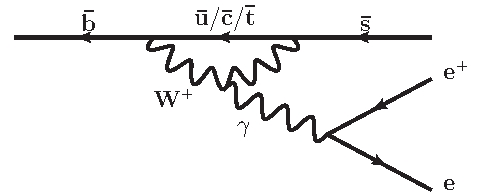
\includegraphics[width=0.45\textwidth]{feynbsg1.jpg}}
   \subfigure{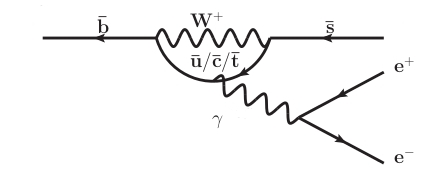
\includegraphics[width=0.49\textwidth]{feynbsg2.jpg}}
  \vspace*{-0.5cm}
  \end{center}
  \caption{\textit{The Feynman diagrams for the \bsg transition.}}
  \label{fig:bsg}
\end{figure}
\newpage
\section{Angular analysis of the \BdKstee}
\label{sec:ksll}
While various ways to measure the photon polarisation have been presented by theorists \cite{ananote} \cite{gross}, the angular analysis of a decay of the form \BdKstll (with $\Kstarz \rightarrow \Kp \pim$) is one of the most promising.\\
This decay proceeds predominantly via the \bsll transition with a virtual photon decaying into two leptons. Since the photon is virtual the kinematics in the \bsll transition are the same as in the \bsg transition, particularly the helicity structure is the same.\\
In \B decays into two vectors (here the virtual photon and the \Kstarz) the subsequent decays of the vectors contain their relative polarisation information \cite{krueger}. Thus, the angular distribution in the relative angles of the $\Kstarz \rightarrow \Kp \pim$ decay plane and the plane of the lepton-pair can be used to determine the helicity amplitudes in the \BdKstll decay and therefore the polarisation amplitudes $A_R$ and ${A_L}$ of the photon.\\

\subsection{Contributions to the \BdKstll Hamiltonian}
The \BdKstll decay proceeds at low lepton-pair invariant mass predominantly via the \bsll transition but other transitions such as the diagram of Figure \ref{fig:bsg} where the photon is replaced by a \Z or the box-diagram in Figure \ref{fig:feynbox} add a non-negligible contribution to the effective Hamiltonian.
\begin{figure}[ht]
\begin{center}
  	\vspace*{-0.5cm}
    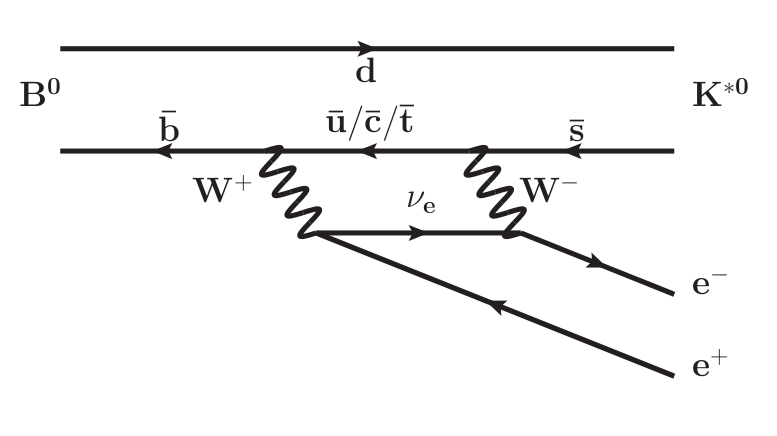
\includegraphics[width=0.48\textwidth]{feynbox.jpg}
  \vspace*{-1cm}
  \end{center}
  \caption{\textit{The box-diagram that contributes to \BdKstll.}}
  \label{fig:feynbox}
\vspace*{-0.5cm}
\end{figure}


The leading order contributions to the \BdKstll effective Hamiltonian (see Equation \ref{eq:genhamilton}) come from the operators $ \Ope7 $ , $ \Ope9 $ and $ \Ope10 $ \cite{krueger}.\\
\begin{eqnarray}
\mathcal{H}_{eff} = -\frac{4G_F }{ \sqrt{2} } \Vtb \Vts^* [& \C7 (\mu) \Ope7 (\mu) + \Cp7 (\mu) \Opep7 (\mu) & \nonumber \\
& \C9 (\mu) \Ope9 (\mu) + \Cp9 (\mu) \Opep9 (\mu) & \ + \ \C10 (\mu) \Ope10 (\mu) + \Cp10 (\mu)\Opep10 (\mu) ]  \nonumber
\label{eq:hamilton}
\end{eqnarray}
with the local operators \cite{gross}
\begin{eqnarray}
& \Ope7 = \frac{e}{16\pi^2} \squarkbar \sigma_{\mu \nu}(m_{\bquark}  P_R \ +\ m_{\squark}P_L)\bquark F^{\mu \nu} &\\
&\Ope9 = \frac{e^2}{16\pi^2} (\squarkbar \gamma_{\mu} P_L \bquark)(\bar{\electron}\gamma^{\mu}\electron) \qquad \Ope10 = \frac{e^2}{16\pi^2} (\squarkbar \gamma_{\mu} P_L \bquark)(\bar{\electron}\gamma^{\mu} \gamma_5 \electron) & \nonumber
\end{eqnarray}

The $ \Ope7 $ corresponds to the SM \bsll transition (\bsg transition) with a left-handed weak-charged current. Since there are no right-handed weak-charged currents in the SM, the $ \Cp7(\mu) $ is only non-zero for contributions from new physics. It is therefore appreciable to measure quantities connected to \Cp7 . 
\\The operators $ \Ope9 $ and $ \Ope10 $ represent the contributions to the \BdKstll decay that do not come from the \bsg transition but for example from the box-diagram in Figure \ref{fig:feynbox}.\\
The branching ratio \BR(\BdKstll) increases significantly towards low $q^2$ values
 (where $q^2$ denotes the square of the dilepton invariant mass)\cite{jaeger}. This is due to the strong increase of the \BR(\bsll) while the other contributions to \BdKstll vary much more smoothly and show no particular increase at low $q^2$. These other contributions make up for a few \% of the events with $20\mevcc < q < 1\gevcc $.\\
At \lhcb the angular analysis of \BdKstll decays is performed with muons and electrons in different bins of $q^2$. The combination of these analyses gives global information about all polarisation amplitudes over a large range of $q^2$ and the relative contributions from $\C9 (\mu)$ and $ \C10 (\mu)$ can be determined. 
\begin{figure}[ht]
  \centering
    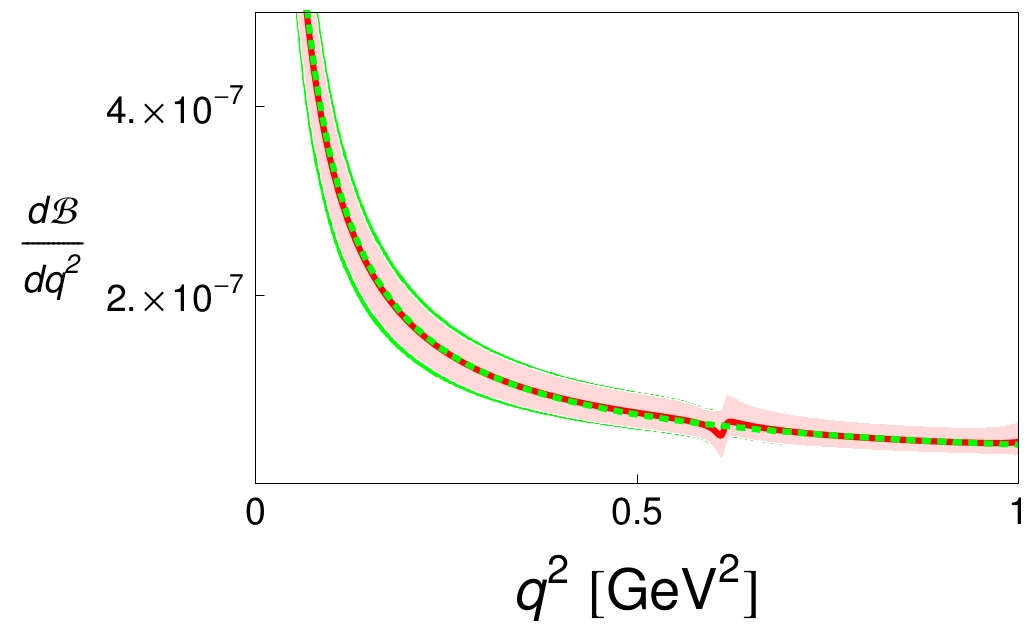
\includegraphics[width=0.55\textwidth]{BR.jpg}
  \caption{\textit{The \BR(\BdKstee) for the low $q^2$ region. Solid (red) and dashed (green) lines correspond to the SM prediction for two different models. The error band is calculated from different theoretical uncertainties such as hadronic and CKM uncertainties and renormalization scale dependence.}\cite{jaeger}}
  \label{fig:BR}
\end{figure}

\subsection{Polarisation amplitudes for the \BdKstee}
\label{sub:polamp}
In the framework of the effective theory, the transversity polarisation amplitudes $A^{L,R}_{ \perp }$, $A^{L,R}_{ \parallel }$ and $A^{L,R}_0$ can be expressed in terms of the Wilson coefficients \cite{krueger}. The indices $L$ and $R$ refer to the chirality of the lepton current. In this calculation the leptons are presumed to be massless which is a very good approximation for the \BdKstee. In the region low $q^2$ region which corresponds to large recoil of the \Kstarz, the amplitudes can be expressed as:
\begin{equation}
A^{L,R}_{ \perp }(q^2) = \frac{ \sqrt{2} N (M^2_B - q^2) }{ M_B }[(\C9 + \Cp9 ) \mp (\C10 + \Cp10 )+\frac{ 2 m_b M_B }{ q^2 } (\C7 + \Cp7 )] \xi_{ \perp }(q^2)
\end{equation}
\begin{equation}
A^{L,R}_{ \parallel }(q^2) = \frac{ \sqrt{2} N (M^2_B - q^2) }{ M_B } [(\C9 + \Cp9 ) \mp (\C10 + \Cp10 )+ \frac{ 2 m_b M_B }{ q^2 }(\C7 - \Cp7 )] \xi_{ \perp }(q^2)
\end{equation}
\begin{equation}
A^{L,R}_0 (q^2) = \frac{ \sqrt{2} N (M^2_B - q^2) }{M_B } [(\C9 + \Cp9 ) \mp (\C10 + \Cp10 )+ \frac{2 m_b }{M_B }(\C7 - \Cp7 )] \xi_{ \parallel }(q^2)
\end{equation}
 
In the above formulae $ \lambda = M_B^4 + M_{\Kstarz}^4 + q^2 - 2(M_B^2 M_{\Kstarz}^2 + M_{\Kstarz}^2 q + M_B^2 q  ) $ and
\begin{equation}
N = \Bigg[ \frac{G_F^2 \alpha^2}{3 \cdot 2^{10}\pi^5 M_B^3} |\Vtb \Vts^* |^2 q \lambda^{1/2} \Big( 1 - \frac{4 m_l^2}{q} \Big)^{1/2} \Bigg]
\end{equation}
and $M_B$: mass of the \B meson, $M_{\Kstarz} $: mass of the \Kstarz meson, $m_b $: mass of the \bquark quark, $m_l $: mass of the lepton. The  $\xi_{ \perp }(q^2)$ and  $\xi_{ \parallel }(q^2)$ factors are the form factors of the \Kstarz meson and contain the non-pertubative physics. As can be seen in those formulae, the polarisation amplitudes are sensitive to new physics that might appear in the Wilson coefficients.\\
Four parameters can be expressed as a combination of the transversity amplitudes and subsequently fitted:
\begin{equation}
F_L(q^2) = \frac{ |A^{L}_0|^2 + |A^{R}_0|^2 }{ |A^{L}_0|^2 + |A^{L}_{ \perp } |^2 + | A^{L}_{ \parallel } |^2 +  |A^{R}_0|^2  + | A^{R}_{ \perp } |^2 + | A^{R}_{ \parallel } |^2 }
\end{equation}
\begin{equation}
A_{FB}(q^2) = \frac{3}{2} \frac{ \Re ( A^L_{ \parallel }( A^L_{ \perp } )^* ) - \Re (A^R_{ \parallel }( A^R_{ \perp } )^* ) }{ | A^L_0 |^2 + | A^L_{ \perp } |^2 + | A^{L}_{ \parallel } |^2 +  | A^{R}_0 |^2  + | A^{R}_{ \perp } |^2 + |A^R_{ \parallel } |^2 }
\end{equation}

\begin{equation}
A^{(2)}_T(q^2) = \frac{|A^{L}_{ \perp }|^2 + |A^{R}_{ \perp }|^2 - |A^{L}_{ \parallel }|^2 - |A^{R}_{ \parallel }|^2 }{|A^{L}_{ \perp }|^2 + |A^{R}_{ \perp }|^2 + |A^{L}_{ \parallel }|^2 + |A^{R}_{ \parallel }|^2}
\end{equation}

\begin{equation}
A^{Im}_T(q^2) = \frac{2 \Im (A^{L}_{ \parallel } (A^{L}_{ \perp })^* + A^{R}_{ \parallel } (A^{R}_{ \perp })^*)}{|A^{L}_{ \perp }|^2 + |A^{R}_{ \perp }|^2 + |A^{L}_{ \parallel }|^2 + |A^{R}_{ \parallel }|^2}
\end{equation}
It can be seen from this formulae that the $A^{(2)}_T(q^2)$ and the $A^{Im}_T(q^2)$ don't depend on the hadronic form factors $\xi_{ \perp }(q^2)$ and $\xi_{ \parallel }(q^2)$ any more, thus a great systematic uncertainty from the theoretical part is removed.\\
The amplitudes for the photon polarisation $A_L$ and $A_R$ can be related to the transversity amplitudes
\begin{equation}
A_{\perp} = \frac{A_R - A_L}{\sqrt{2}} \qquad \qquad  A_{\parallel} = \frac{A_R + A_L}{\sqrt{2}}
\end{equation}
and to $A^{(2)}_T$
\begin{equation}
A^{(2)}_T(q^2) = -2 \Re \Big( \frac{A^*_R(q^2)A_L(q^2)}{|A_R| ^2+ |A_L|^2} \Big) \sim - 2\, \frac{A_R}{A_L}
\end{equation}
The approximation holds up if $\frac{A_R}{A_L}$ is small and real.
%For the low invariant dilepton mass limit $q^2 \rightarrow 0$ the contributions from the Wilson coefficients \Ope9 and \Ope10 become negligible and the amplitude $A^{(2)}_T(q^2)$ can be simplified to
%\begin{equation}
%A^{(2)}_T(q^2 \rightarrow 0) = \frac{2 \Re ( \C7 \, (\Cp7 )^*)}{| \C7 |^2 + | (\Cp7 )^*|^2} = 2\, \frac{A_R}{A_L}
%\end{equation}
This shows clearly that the variable $A^{(2)}_T(q^2)$ is the one that contains the information about the photon polarisation.\\
\newpage
\subsection{Angular distribution}
\label{sec:angles}
The \BdKstll decay is completely defined by four independent kinematic variables; namely the lepton-pair invariant mass $q$ and the three angles $\theta_l$, $\theta_K$ and $\Phi$ which are illustrated in Figure \ref{fig:winkel} \cite{krueger} \cite{ananote}. The angles are defined as:
\begin{itemize}
\item $\theta_l$: the angle between the direction of the vector of the \en (\ep) in the dilepton rest frame, and the direction of the dilepton in the $B^0$ ($\bar{B}^0$) rest frame
\item $\theta_K$: the angle between the direction of the vector of the \pion in the \Kstarz (\Kstarzb) rest frame, and the direction of the \Kstarz (\Kstarzb) in the $B^0$ ($\bar{B}^0$) rest frame
\item $\Phi$: the angle between the planes defined by the \Kstarz daughters and the dileption daughters, in the rest frame of the \B meson.
\end{itemize}

\begin{figure}[!h]
  \begin{center}
  	\vspace*{-0.5cm}
 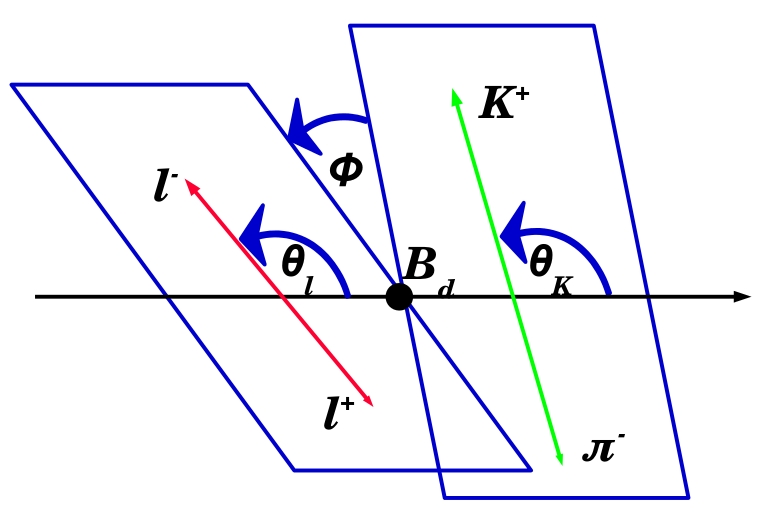
\includegraphics[width=0.6\textwidth]{winkel.jpg}
  \vspace*{-0.8cm}
  \end{center}
  \caption{\textit{Definition of the angles $\theta_l$, $\theta_K$ and $\Phi$ in the \BdKstll decay.}}
  \label{fig:winkel}
\end{figure}

The normalized differential decay width can be expressed as
\begin{equation}
\frac{1}{\Gamma}\frac{d^4 \Gamma}{dq^2 \, \ctl \, \ctk \, d\Phi} = \frac{9}{32 \pi}\sum_{i=1}^{9} I_i'(q^2, \theta_K) f_i(\theta_l , \Phi)
\end{equation}
where the $I_i'$ depend on $q^2$, $\theta_K$ and the helicity polarisation amplitudes $F_L(q^2)$, $A_{FB}(q^2)$, $A^{(2)}_T(q^2)$ and $A^{Im}_T(q^2)$. The $f_i$ are the corresponding angular distribution functions
\begin{eqnarray}
f_1 = 1 \qquad & f_2 = \cos(2\theta_l) \qquad & f_3 = \sin^2(\theta_l) \cos(2\Phi)\nonumber\\
f_4 = \sin(2\theta_l) \cos(\Phi) \qquad & f_5 = \sin(\theta_l) \cos(\Phi) \qquad & f_6 = \cos(\theta_l)\\
f_7 = \sin(\theta_l)\sin(\Phi) \qquad & f_8 = \sin(2\theta_l)\sin(\Phi)\qquad & f_9 = \sin^2(\theta_l)\sin(2\Phi)\nonumber
\end{eqnarray}
The $I_i$ which are sensitive to the ratio of photon polarisations $\frac{A_R}{A_L}$ are $I_3$ and $I_9$. The partial decay width can then be simplified without any loss in information about the photon polarisation by folding the angular distributions for $\Phi$ and $\theta_l$. $\Phi$ is folded by moving all values with $\Phi <0$ to $\Phi + \pi$. This removes the terms proportional to $\cos(\Phi)$ and $\sin(\Phi)$ without affecting the $\cos(2\Phi)$ and $\sin(2\Phi)$ terms. The angle $\theta_l$ is folded by mapping the interval $(\pi /2, \pi)$ onto $(0, \pi /2)$ which removes the term proportional to $\cos(\theta_l)$. 
The decay width after these transformations and neglecting the lepton mass term -- which is legitimate for the \BdKstee decay where $\frac{m^2_{\electron}}{q^2} << 1$ -- is
 \begin{eqnarray}
 \frac{1}{\Gamma}\frac{d^4\, \Gamma}{dq^2 \, \ctl \, \ctk \, d\Phi} = \frac{9}{32 \pi} [  I_1'(q^2, \cos\theta_K)\ +   I_2'(q^2, \cos\theta_K)\, (2\cos^2\theta_l -1) \nonumber \\
  +  I_3'(q^2, \cos\theta_K)\, \sin^2\theta_l \, \cos2\Phi \ +  I_9'(q^2, \cos\theta_K)\, \sin^2\theta_l \, \sin2\Phi ]
 \label{eq:partw}
 \end{eqnarray}
The $I_i'$ terms can be expressed as
\begin{eqnarray}
 I_1'(q^2, \cos\theta_K) &=& \frac{3}{4} (1-F_L(q^2)) \cdot (1-\cos^2\theta_K) + F_L(q^2) \cdot \cos^2\theta_K \nonumber \\
 I_2'(q^2, \cos\theta_K) &=& \frac{1}{4} (1-F_L(q^2)) \cdot (1-\cos^2\theta_K) - F_L(q^2) \cdot \cos^2\theta_K \nonumber \\
 I_3'(q^2, \cos\theta_K) &=& \frac{1}{2} (1-F_L(q^2)) \cdot A^{(2)}_T(q^2) \cdot (1 - \cos^2\theta_K)   \label{eq:is} \\
   I_9'(q^2, \cos\theta_K) &=& \frac{1}{2} (1-F_L(q^2)) \cdot A^{Im}_T(q^2) \cdot (1 - \cos^2\theta_K)  \nonumber 
\end{eqnarray}
By performing an angular analysis, all three remaining parameters $F_L(q^2)$, $A^{(2)}_T(q^2)$ and $A^{Im}_T(q^2)$ can be fitted at the same time and the information about the photon polarisation can be extracted. \\

\subsection{The advantages of the low $q^2$ bin in \BdKstee}
This masters thesis is part of an angular analysis that focusses on the low dilepton invariant mass $q$ region in the \BdKstee decay.\\
The choice of performing the analysis with electrons as opposed to with muons is that the sensitivity to new physics -- which could affect the photon polarisation -- is increased. This is due to the fact that the electron mass is negligible compared to $q^2$: $m^2_e<< q^2$. For a non-negligible lepton mass the $I_3'$ and $I_9'$ in Equations \ref{eq:is} are multiplied by $(1-x)$ with $ x = \frac{4m^2_{l}}{q^2}$ which thus degrades the sensitivity on $A^{(2)}_T(q^2)$ and $A^{Im}_T(q^2)$. In addition the kinematically allowed $q^2$ range is larger.\\
The choice of $20 \mevcc < q < 1\gevcc $ has two distinct advantages. The first advantage is that the contribution coming from the non-\bsll transitions in \Ope9 and \Ope10 are very small (a few \%) and therefore $A^{(2)}_T(q^2) \sim -2\, \frac{A_R}{A_L}$\footnote{Note that the angles in Section \ref{sec:angles} are defined such that for each the \bsll and the \bbsll decay $A^{(2)}_T(q^2)$ corresponds to the ratio of suppressed amplitude over favoured amplitude.} (see Section \ref{sub:polamp}). The analysis of the \BdKstee decay at low $q^2$ is therefore directly sensitive to the \bsll transitions and the photon polarisation. The second advantage of constraining the dilepton invariant mass lies in the $q^2$ dependence of the $F_L(q^2)$ amplitude shown in Figure \ref{fig:sens}. $F_L(q^2)$ is low for small $q^2$ values and increases with $q^2$. Since the amplitude $A^{(2)}_T(q^2)$ appears in $I_3'$ in Equation \ref{eq:is} in combination with $(1-F_L(q^2))$ the sensitivity to $A^{(2)}_T(q^2)$ is highest for low $q^2$. \\
The effects of the low lepton mass of the electrons opposed to muons combined with the effects of $q^2$ on $F_L(q^2)$ are shown in Figure \ref{fig:sens}.\\
\begin{figure}[ht]
\vspace*{-0.5cm}
  \begin{center}
  	\subfigure{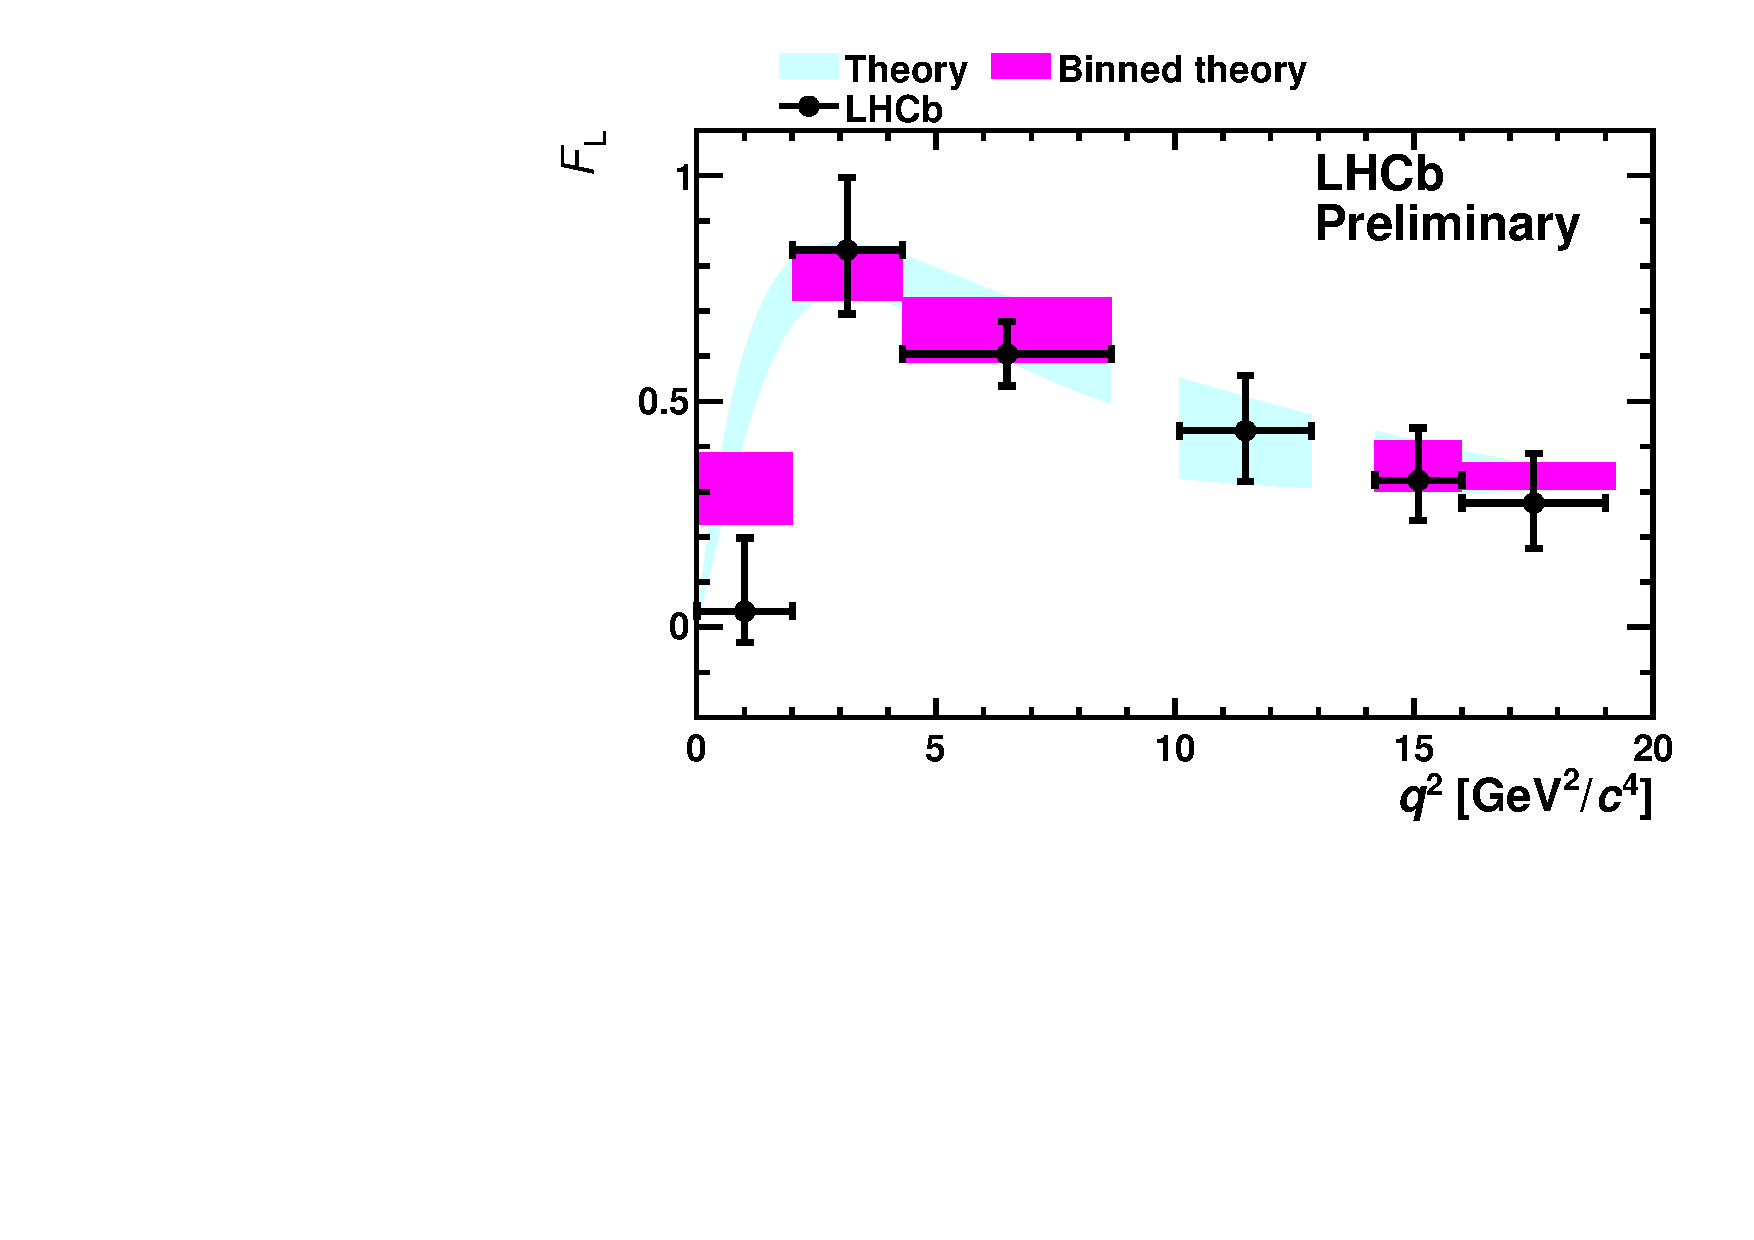
\includegraphics[width=0.52\textwidth]{Fl.pdf}}
   \subfigure{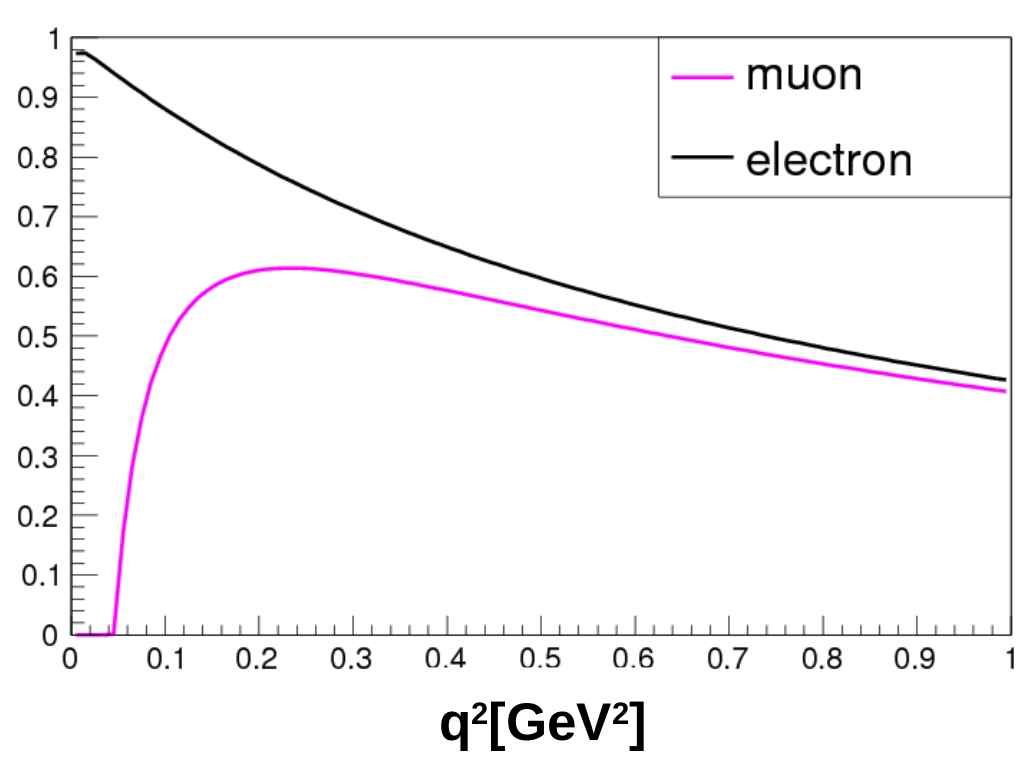
\includegraphics[width=0.47\textwidth]{sensitivity.jpg}}
  \vspace*{-0.5cm}
  \end{center}
  \caption{\textit{The parameter $F_L(q^2)$ (left) and the sensitivity on the parameter $A^{(2)}_T(q^2)$ for muons and electrons (right). $F_L(q^2)$ was determined by analysis of $\Bd \rightarrow K^{*0} \mup \mun$ for different bins of $q^2$.}\cite{mumu}}
  \label{fig:sens}
\end{figure}

\subsection{The lower cut: $q\, > 20\mevcc$}
Although the \BdKstee events at low $q^2$ carry the most information about the photon polarisation a cut of $q\, > 20\mevcc$ has to be performed. At dielectron invariant mass $m(\epem)\approx 0$ the two electrons are nearly collinear and therefore the angle between them is very small. At the limit of $q^2 \rightarrow 0$ the dilepton plane cannot be defined any more and thus the $\Phi$ angle cannot be determined. By experiencing multiple scattering of the electrons in the detector the plane defined by the (\epem) pair is extremely distorted. This leads to a great uncertainty on the $\Phi$ angle which makes these events useless for the angular analysis. Furthermore the measured (\epem) invariant mass is increased due to added opening angle between the electron and the positron due to multiple scattering. \\
To allow for a small uncertainty on the measured $\Phi$ angle a study has been performed on the resolution of the $\Phi$ angle. Figure \ref{fig:phires} shows the resolution of the $\Phi$ angle with respect to the invariant mass of the electron pair. The uncertainty on $\Phi$ drops off exponentially and remains stable from $150 \mevcc$ onwards.\\
The cut of $q\, > 20\mevcc$ was chosen as the $\Phi$ resolution is acceptable at from this value on. This cut also allows to keep a large amount if events with low electron pair invariant mass.
\begin{figure}[ht]
\vspace{-0.4cm}
  \begin{center}
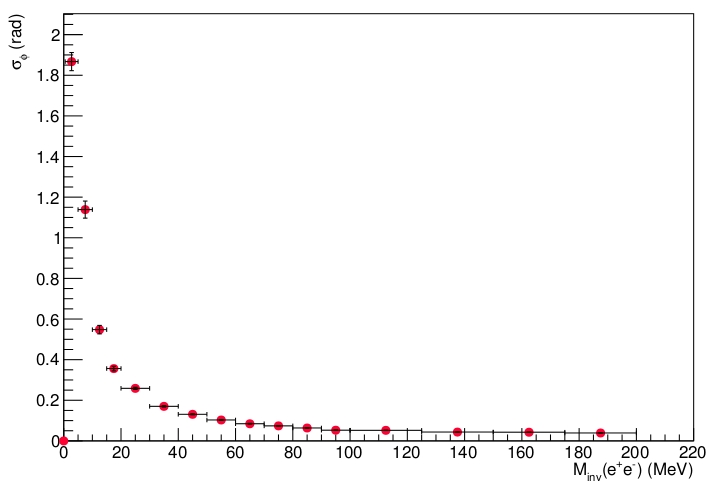
\includegraphics[width=0.5\textwidth]{phires.jpg}
  \vspace*{-0.8cm}
  \end{center}
  \caption{\textit{The resolution of the $\Phi$ angle for different bins of (\epem) invariant mass obtained from \BdKstee Monte Carlo.}}
  \label{fig:phires}
\end{figure}
%\chapter{The \lhcb experiment}
\chaptermark{Chapter3}
\label{chapter2}
%\addcontentsline{toc}{chapter}{The \lhcb experiment}
\lhcb is one of the four large experiments allocated at the Large Hadron Collider (\lhc). It is dedicated to the study of \CP violation and the search for new physics in rare decays of \B and \D mesons. As much focus is put on precision measurements of SM parameters as on the indirect detection of new physics that can intervene in loop and penguin diagrams.\\
The \lhc provides an ideal environment for new research in the sector of heavy flavour physics. The nominal center of mass energy of the \lhc was $\sqrt{s}=7\tev$ in 2011 and $\sqrt{s}=8\tev$ in 2012. The according \bbbar production cross sections at the hadron collider are $\sigma_{\bbbar}(7\tev)= 251.8\, \mu b$ and $\sigma_{\bbbar}(8\tev)= 291.6\, \mu b$ \cite{pythia} resulting in $6.5 \cdot 10^{11}$ \B hadrons produced in the \lhcb detector acceptance in both years combined ($3\invfb$ integrated luminosity collected in 2011 + 2012). 
Additionally to providing high statistics, the \lhc gives access to the system of the $B_s$ meson -- which was mostly beyond the reach of previous \bquark factories such as \babar and \belle \ -- allowing for the investigation of \CP violation and the search for new physics in the \Bs system.\\ 
The \lhcb collaboration has already published several new results constraining SM parameters and possible contributions from new physics, for example the restraining of SUSY parameters with the decays $B^0_s \rightarrow \mup \mun$ and $B^0 \rightarrow \mup \mun$ \cite{bsmumu}.\\
\\
This chapter is dedicated to the description of the \lhcb detector. After a general overview over the detector the different subdetectors of the tracking system and the particle identification system are presented and a summary of the detector performance is given. Then the \lhcb trigger system and different trigger lines are introduced. At the end of this chapter \lhcb software is introduced. \\
 
\section{The \lhcb detector}
\label{sec:lhcb}
The \lhcb detector was designed as a single arm forward spectrometer \cite{lhcbletter} to match the kinematics of \bbbar production shown in Figure \ref{fig:pseudorapidity}. Corresponding to this distribution, the \lhcb detector covers an angular range of $10\,$mrad$\, - \, 300 \,$mrad in the bending and $10\,$mrad$\, - \, 250 \,$mrad in the non-bending plane. Both for $7\tev$ and $8\tev$ $25\,\%$ of the produced \bbbar pairs are in the detector acceptance.\\
\\
To enable precision measurements, the \lhcb detector was build with a minimal amount of material budget. Additionally, the \lhc conducts luminosity levelling for \lhcb. The proton-beams are tuned to be displaced with respect to each other at the \lhcb collision point, giving the bunches only a small overlap while colliding. The luminosity levelling is performed in a manner that keeps the number of proton-proton interaction per bunch-crossing adjusted to an average of $1.5$ throughout the entire run.\\
\\
The \lhcb detector is composed of several subdetectors shown in Figure \ref{fig:lhcb} and presented in the following sections.
Altogether the \lhcb detector incorporates precision vertexting and tracking, worldwide leading particle identification and efficient triggering through a system of dynamic triggers.
 \begin{figure}[ht]
  \begin{center}
  \subfigure{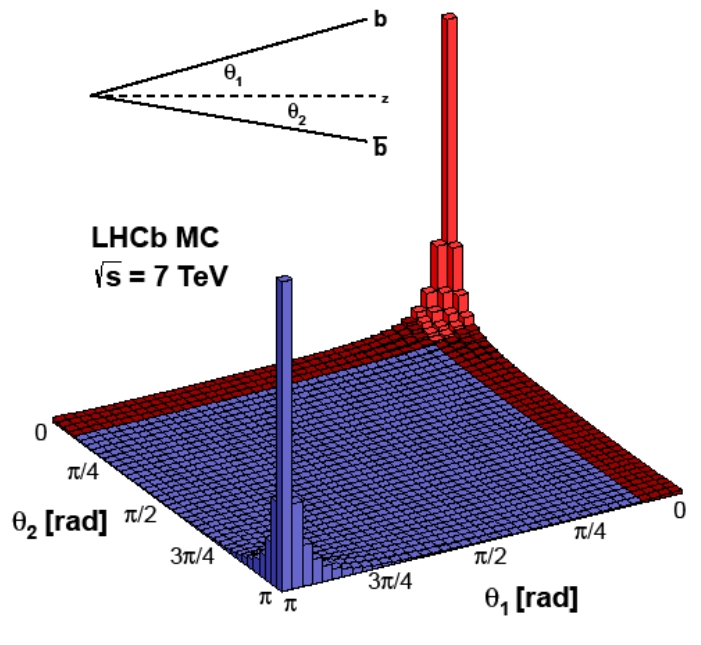
\includegraphics[width=0.4\textwidth]{pseudorapidity.jpg}}
    \subfigure{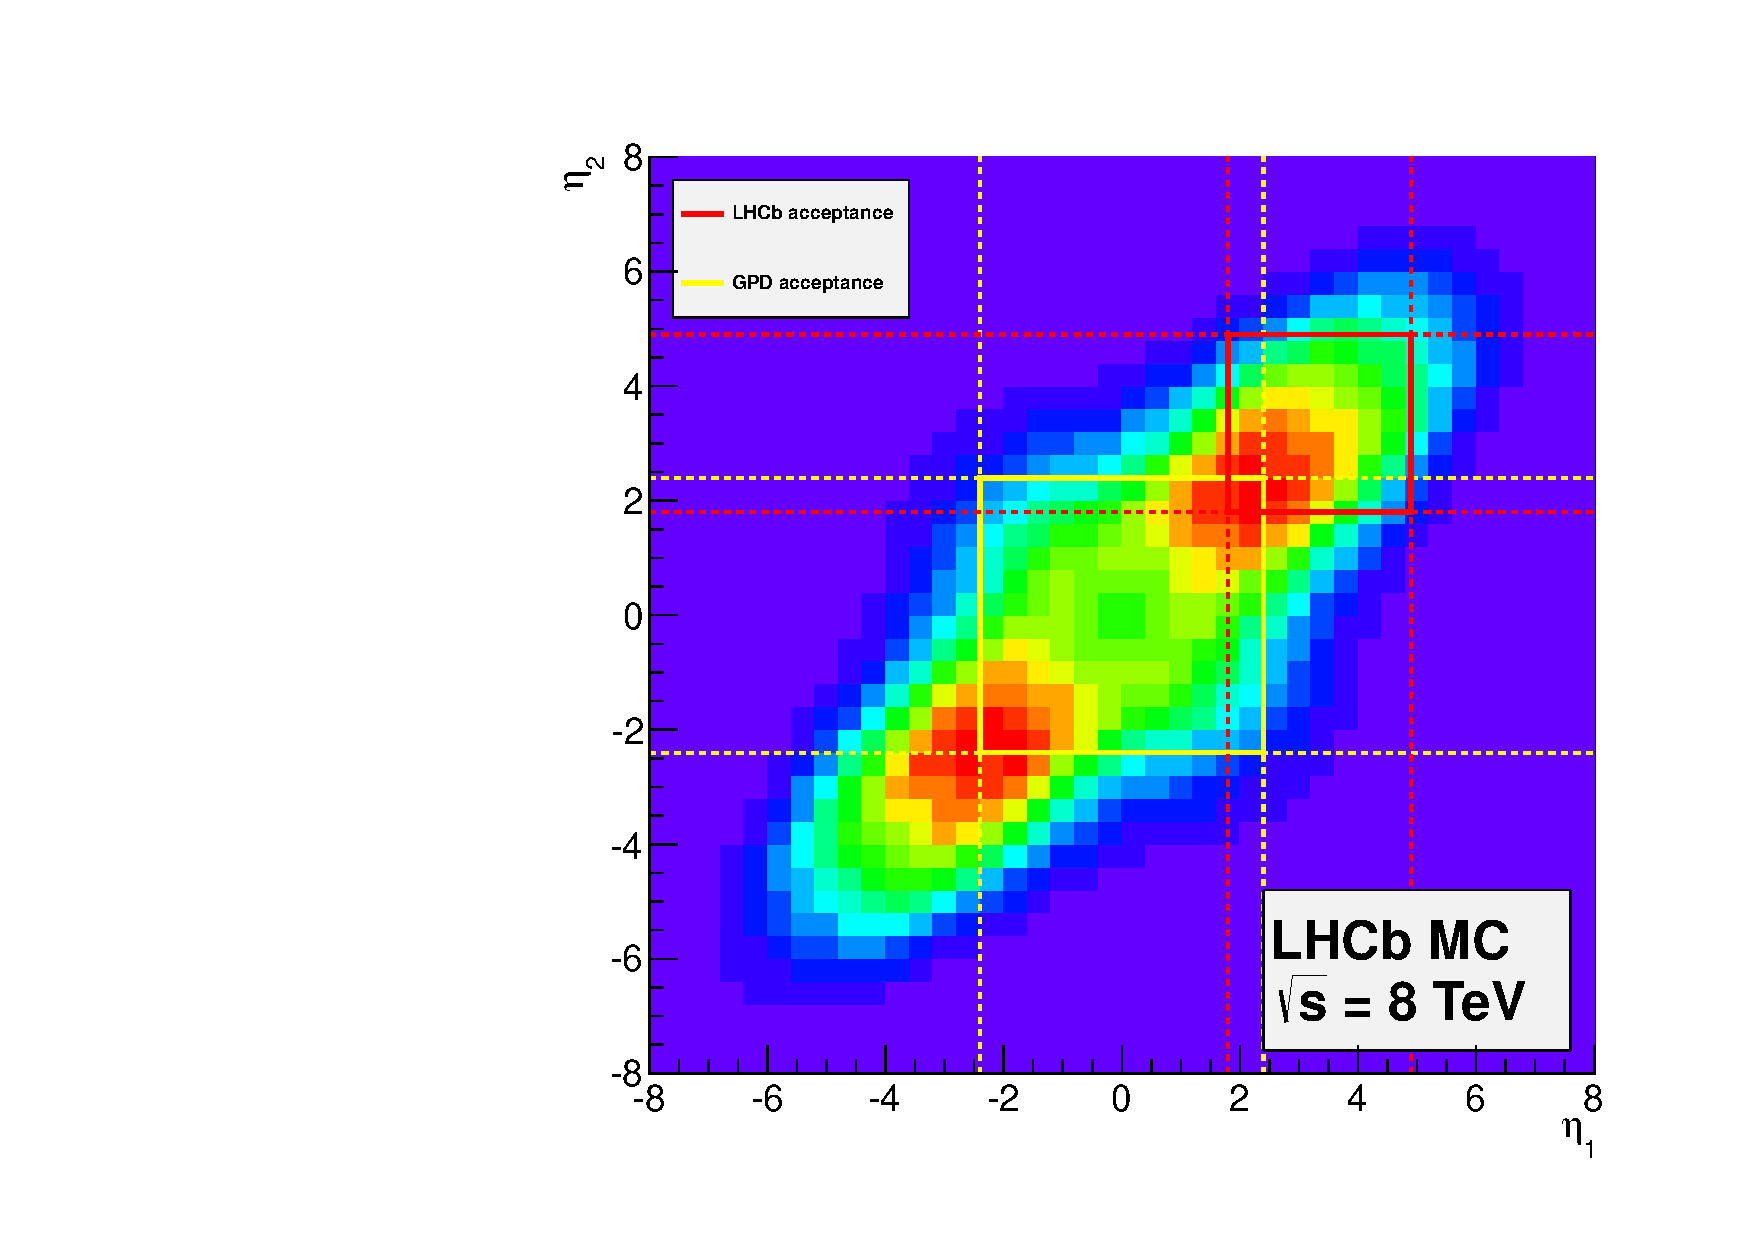
\includegraphics[width=0.42\textwidth]{acceptance.pdf}}
  \vspace*{-0.5cm}
  \end{center}
  \caption{\textit{Angular distribution of \bbbar produced in proton-proton collisions. At hadron colliders the dominant mechanism for \bbbar production is through gluon gluon fusion. Due to the statistical partition of the energy inside the protons the \bbbar pairs originated from the gluon gluon interactions are boosted in the forward or backward direction.}\cite{pythia}}
  \label{fig:pseudorapidity}
\end{figure}
\newpage

\noindent%
\begin{minipage}{\linewidth}
\makebox[\linewidth]{%
  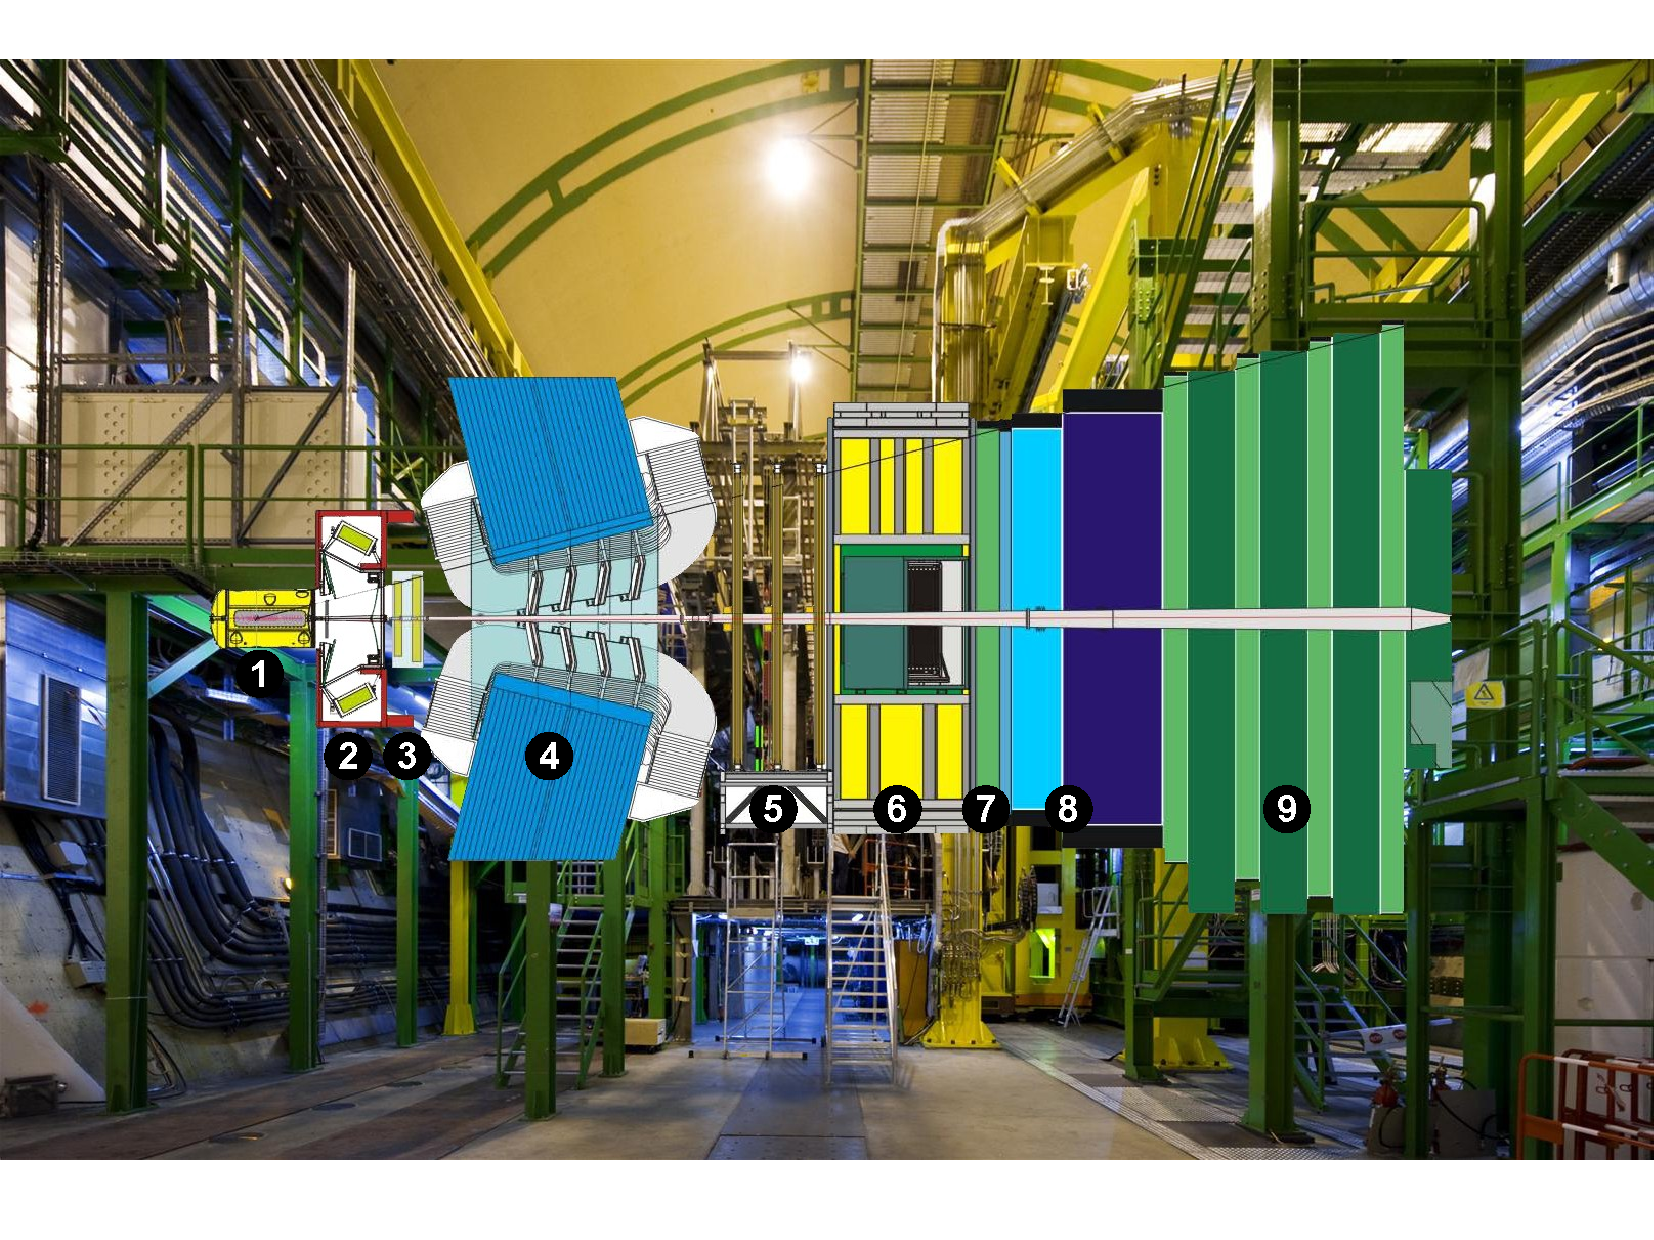
\includegraphics[angle=90, width=0.95\textwidth]{lhcb.pdf}}
\captionof{figure}{\textit{The \lhcb detector. 1: Vertex Locator (\velo), 2: Ring Imaging Cherenkov detector 1 (\richone), 3: Tracker Turicensis (\ttracker), 4: the magnet, 5: the tracking stations, 6: Ring Imaging Cherenkov detector 2 (\richtwo), 7: Muon chamber 1 (\Mone), 8: Scintillating Pad Detector (\spd), PreShower Detector (\presh), electromagnetic calorimeter (\ecal) and hadronic calorimeter (\hcal), 9: Muon chambers 2 to 5 (\Mtwo to \Mfive).}\cite{lhcb}}
  \label{fig:lhcb}
\end{minipage}
\newpage

\subsection{The tracking system}
The \lhcb tracking system's purpose is the detection of charged particle tracks and the measurement of their momenta. It is also responsible for the reconstruction of production and decay vertices of \B and \D mesons. This is essential not only for lifetime measurements but also for an efficient background rejection in the analysis of rare decays.\\
The tracking system consists of the Vertex Locator (\velo), the magnet, the Silicon Tracker (\st) and the Outer Tracker (\ot). The Silicon Tracker makes up for the entire Tracker Turicensis (\ttracker) and the Inner Tracker (\intr) which is the inner part of the three tracking stations (\Tone, \Ttwo and \Tthree) downstream of the magnet. The Outer Tracker is the outer part of the tracking stations (see 5. in Figure \ref{fig:lhcb}).
\\
%% Measure the momentum of charged particles

\subsubsection{The Vertex Locator (\velo)}
The \velo \cite{velo} accurately measures the positions of tracks close to the interaction point and allows for a very precise reconstruction of the primary vertex and the impact parameters of all tracks.\\
As shown in Figure \ref{fig:velo}, the vertex locator is approximately $1 \m$ long and consists of 21 disc-like modules arranged around the beam pipe. Each module is composed of two halfs, each having two sides with silicon strips arranged to measure the $R$ and $\Phi$ coordinate respectively. The modules can be approached as close as $8\mm$ to the beam and have a total radius of $4.2 \cm$. The strip pitch varies from $38 \mum $ wide strips nearest to the beam pipe to $102 \mum$ wide strips for the $R$ sensors and $79 \mum$ wide strips for the $\Phi$ sensors at the outer margin according to the particle density in the detector.\\
\begin{figure}[h]
  \begin{center}
  	\vspace*{-0.8cm}
    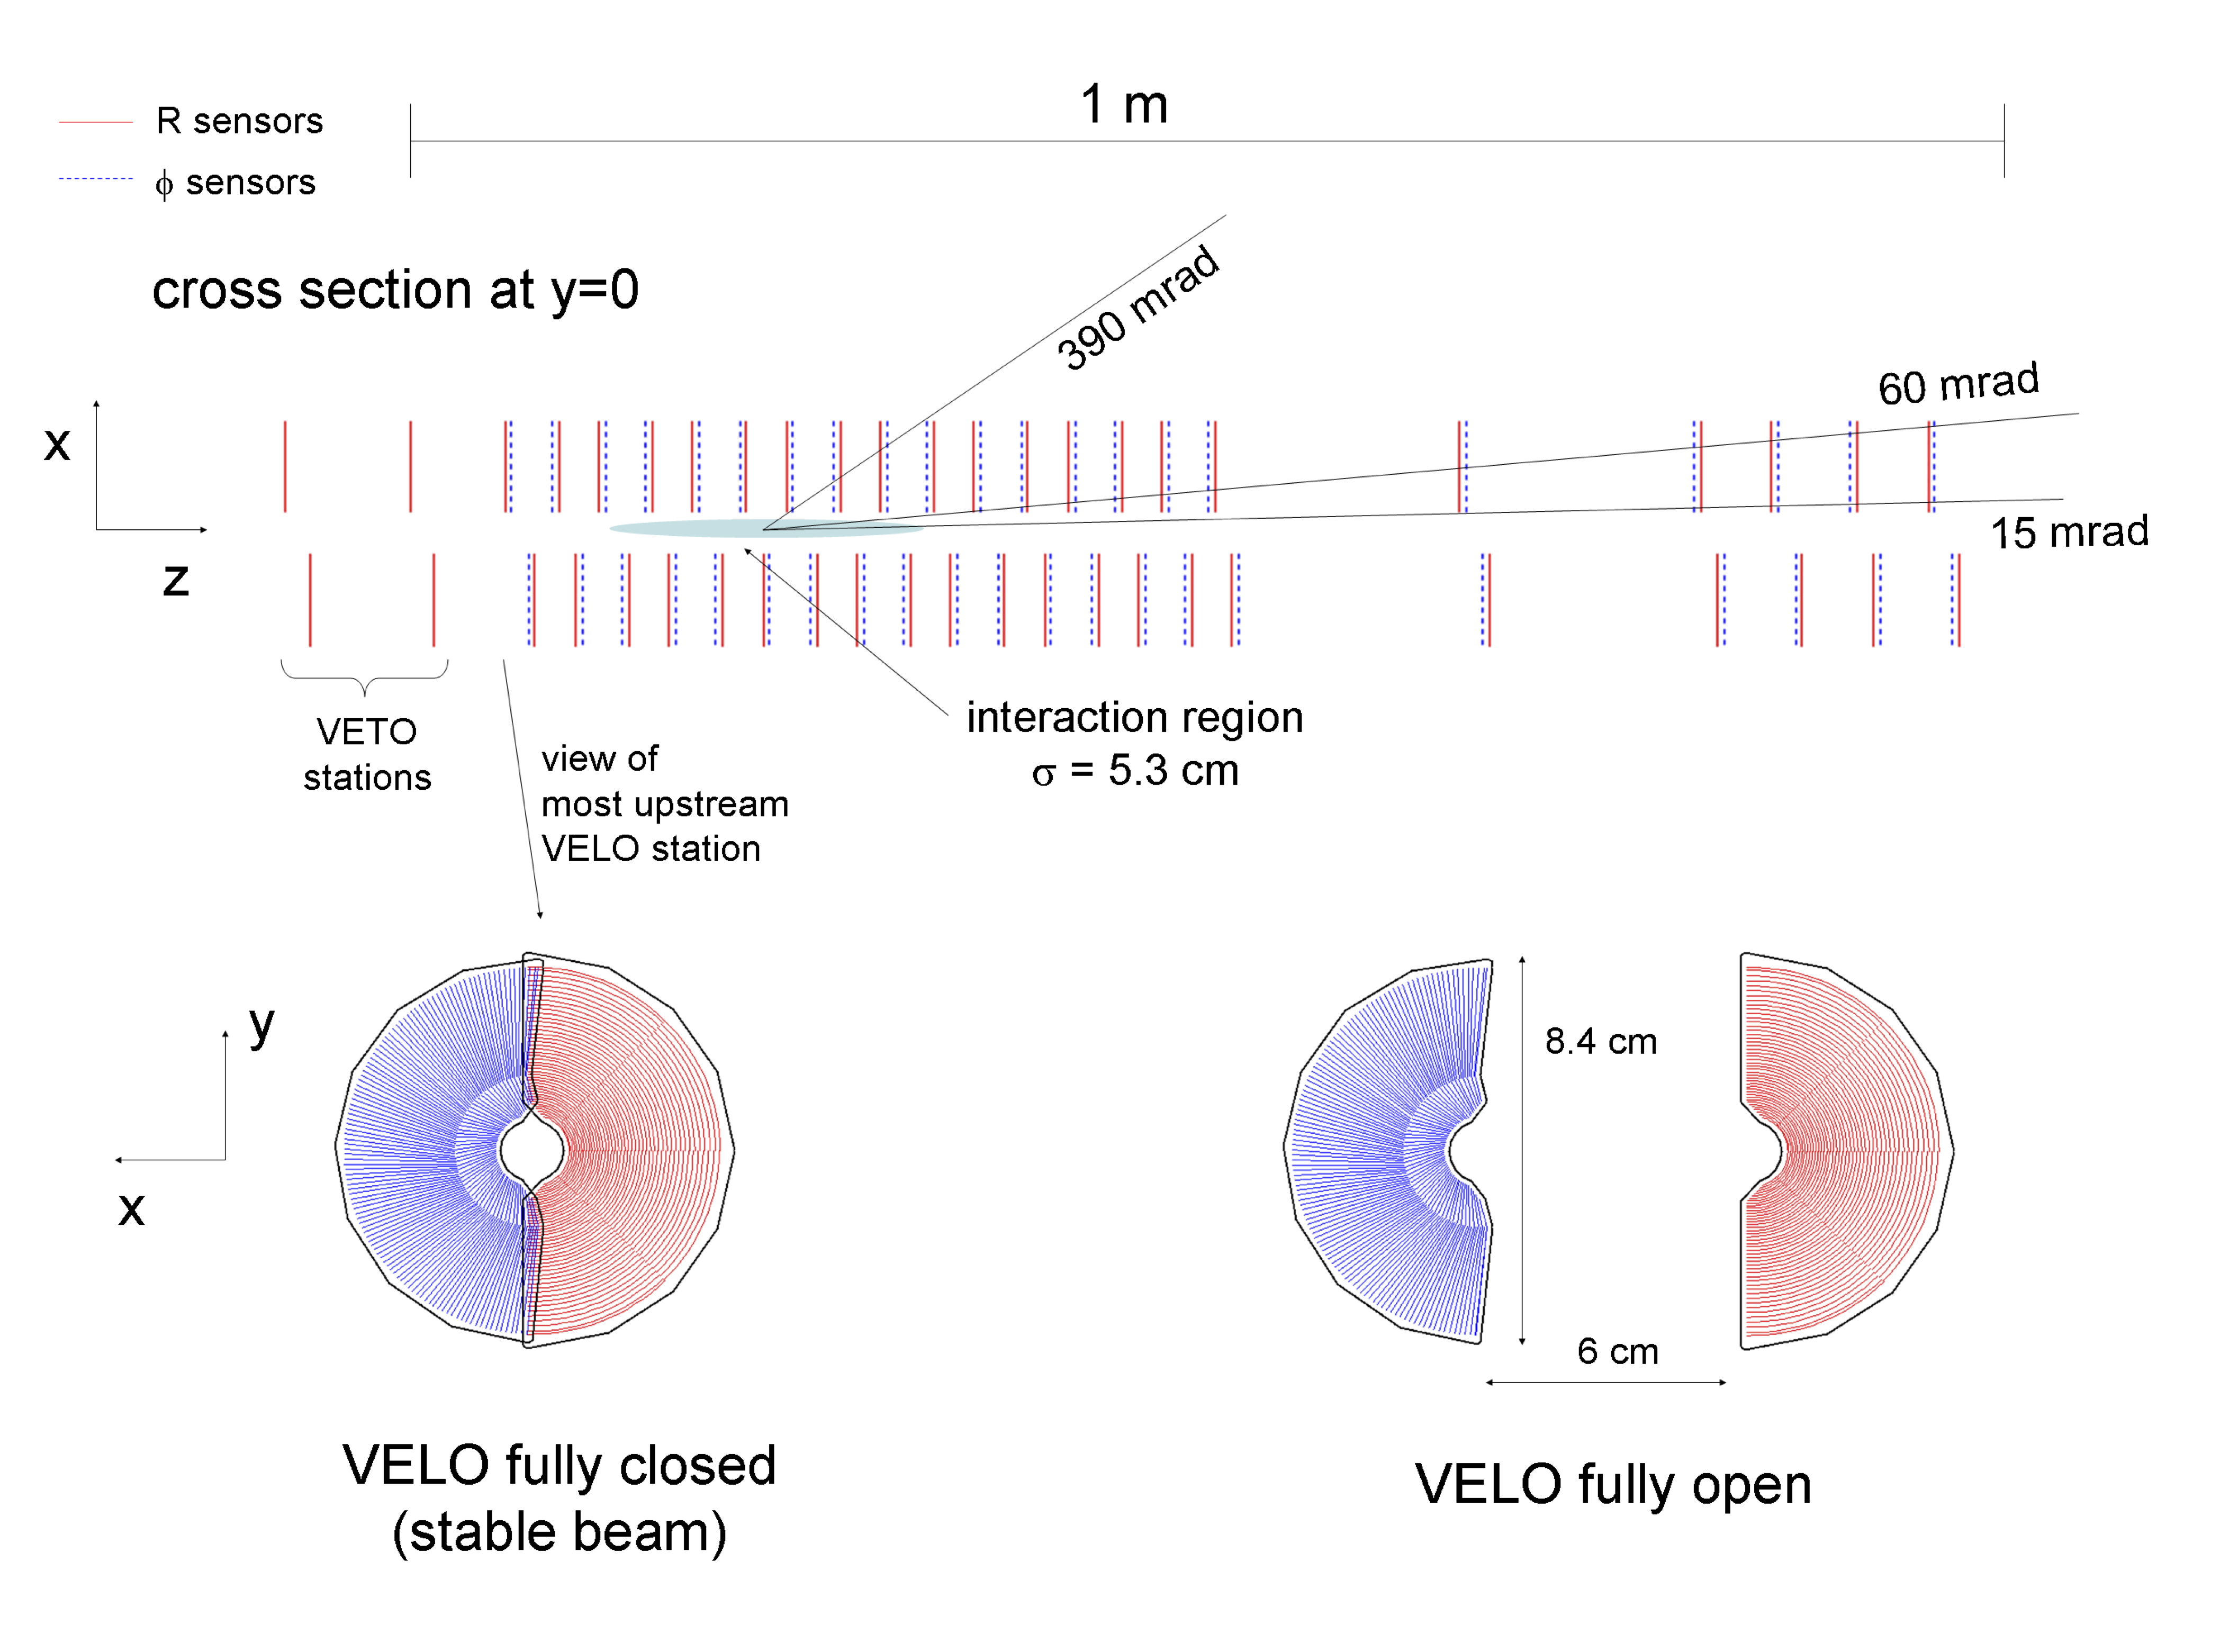
\includegraphics[width=0.75\textwidth]{velo.png}
  \vspace*{-1.0cm}
  \end{center}
  \caption{\textit{Schematic illustration of the \velo. Top: top view of the 21 modules. Bottom: Two \velo modules shown with both halfs to measure $\Phi$ (blue) and $R$ (red). Module in closed position (left) and in open position (right) which is engaged while unstable beam conditions.}\cite{velo}}
  \label{fig:velo}
\end{figure}


\subsubsection{The magnet}
The \lhcb magnet \cite{magnet} is a warm dipole magnet with saddle shaped coils. The streamlines of the magnetic field are parallel to the $y$ axis, making the $(x-z)$ plane the bending plane. Since the relative momentum resolution varies with 
\begin{equation}
\frac{\sigma_p}{p} \propto \frac{1}{B}
\end{equation}
the integrated magnetic field was chosen to be $4\, $Tm. Additionally, the magnet polarisation is regularly changed to reduce systematic effects on measurements due to geometrical acceptances.

\subsubsection{The Silicon Tracker (\st)}
The \st \cite{it} implements silicon microstrip technology for the Tracker Turicensis (\ttracker) and the Inner Tracker (\intr) with a strip pitch of about $200 \mum$. Combining the \ttracker and the \intr, the \st has four stations. Each of this four stations consists of four layers that are arranged in a $(x-u-v-x)$ geometry with vertical strips in the $x$ layers and strips rotated by a stereo angle of $-5^{\circ}$ and $+5^{\circ}$ in the $u$ and $v$ layer respectively.\\
The \ttracker is located upstream of the magnet and allows reconstruction of low momentum particles which are swept out of the detector acceptance after entering the magnetic field. It also provides information for the trigger by performing transverse momentum measurements for tracks with a large impact parameter.
With an area of $140 \cm$ width and $120 \cm$ height, the \ttracker covers the total \lhcb angular acceptance. As can be seen in Figure \ref{fig:st}, the layers of the \ttracker are divided into three different types of sectors ($K$, $M$ and $L$). According to the particle flux that is highest close to the beam pipe and drops of radially, the length of the silicon strips increases from the innermost to the outermost sensors.\\
The \intr covers the inner region of the tracking stations where the particle flux is highest. One layer of the \intr can be seen in Figure \ref{fig:st} on the right. It consists of four pieces arranged in a criss-cross pattern around the beam pipe that cover a total area of $0.35 \m^2$. 
%Each piece contains seven detector modules made out of one or two silicon sensors. The silicon sensors each carry about $400$ silicon microstrips.
\begin{figure}[ht]
  \begin{center}
  \vspace*{-0.cm}
  \subfigure{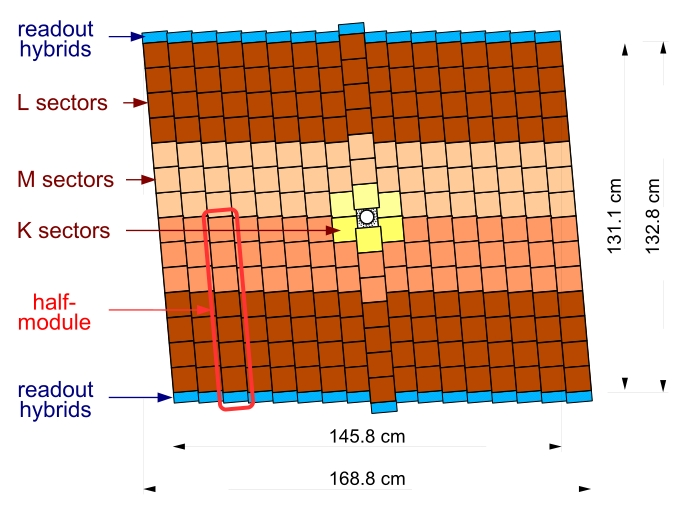
\includegraphics[width=0.49\textwidth]{tt.jpg}}
    \subfigure{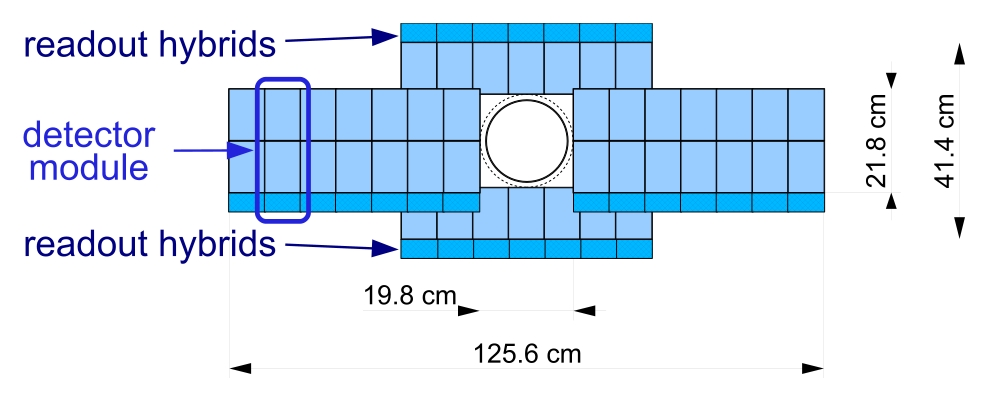
\includegraphics[width=0.49\textwidth]{it.jpg}\vspace{5cm}}
  \vspace*{-1.0cm}
  \end{center}
  \caption{\textit{The two parts of the Silicon Tracker (\st). The Tracker Turicensis (\ttracker) with the three different types of modules (left) and the Inner Tracker (\intr) which is part of the tracking stations (right).}\cite{it}}
  \label{fig:st}
\end{figure}



\subsubsection{The Outer Tracker (\ot)}
The \ot \cite{ot} covers the outer region of the tracking stations. Since the particle flux is lower in this area the \ot implements the technology of drift tubes.
As for the \st, each \ot tracking station has four layers arranged in a $(x-u-v-x)$ geometry with vertical strips in the $x$ layers and strips rotated by a stereo angle of $-5^{\circ}$ and $+5^{\circ}$ in the $u$ and $v$ layer respectively. Each layer covers the total \lhcb angular acceptance. The inner boundaries filled by the \intr were determined by the requirement that occupancies in the straw-tubes should not exceed $10\%$ at the nominal running luminosity of $2\cdot 10^{32} \cm^{-2}s^{-1}$.\\
The structure of the \ot layers is shown in Figure \ref{fig:ot}. Each layer is  build of two different types of modules. All modules are composed of two staggered layers (monolay-
\begin{figure}[ht]
  \begin{center}
  	\vspace*{-0.5cm}
    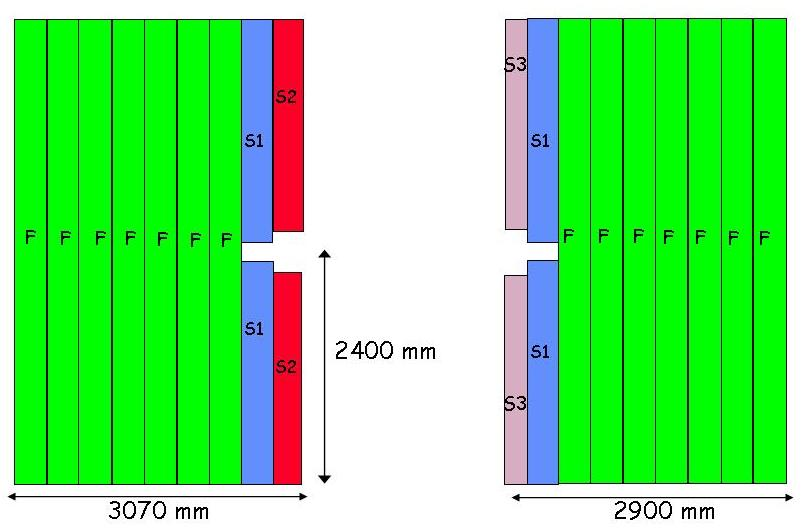
\includegraphics[width=0.45\textwidth]{OT-Modules.jpg}
  \vspace*{-0.5cm}
  \end{center}
  \caption{\textit{One layer of the Outer Tracker (\ot) with the long $F$ modules and the shorter $S$ modules combined out of $256$ and $128$ drift tubes respectively.}\cite{ot}}
  \label{fig:ot}
\end{figure}
ers) of straw-tubes.
The $F$ modules are $4.85\m$ long and consist of $256$ straw-tubes. Their monolayers are split along the $y$ axis, at different positions for each monolayer to avoid insensitive regions in the middle of the modules.
The $S$ modules are shorter than the $F$ modules and located above and below the beam pipe. Each of the $S$ modules has $128$ straw-tubes.\\
All straw-tubes are $5 \mm$ thick and filled with a gas mixture of $Argon$ and $CO_2$ ($70:30$) which combines fast response time ($<50 \ns$) with a high resolution of the drift coordinate ($200\mum$).\\


%\subsubsection{Performance}
%The \lhcb tracking system has an average relative momentum resolution of $0.5 \%$. \\
%The resolution of the $x$ and $y$ coordinates of the primary vertex and the resolution on the impact parameter's $x$ coordinate are shown in Figure \ref{fig:resolution}. For 25 tracks a resolution of $13 \mum$ on the $x$ and $y$ coordinates and a resolution of $69 \mum$ on the $z$ coordinate of the primary vertex can be reached. Additionally and equally excellent impact parameter resolution of $<35 \mum$ for tracks with a transverse momentum $p_T>1 \gev$ can be obtained.
%\begin{figure}[ht]
%  \begin{center}
%  \subfigure{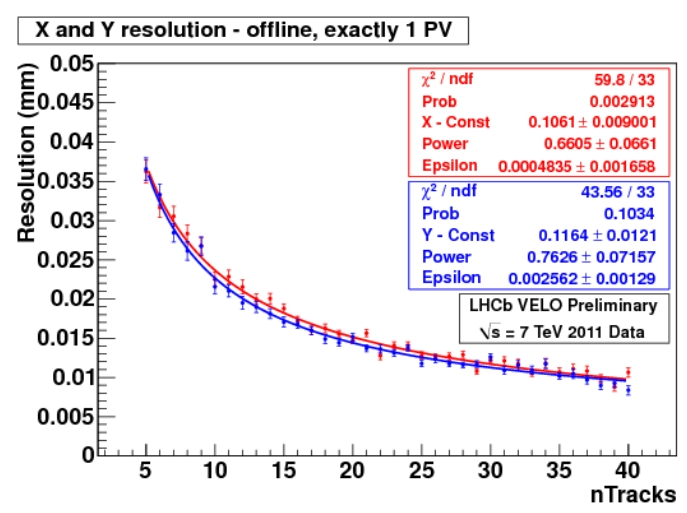
\includegraphics[width=0.45\textwidth]{PVresolution.jpg}}
%    \subfigure{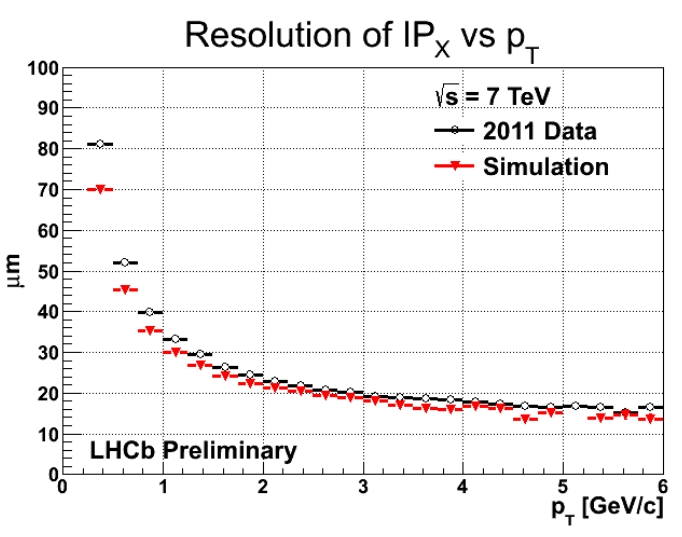
\includegraphics[width=0.45\textwidth]{IPresolution.jpg}}
%  \vspace*{-1.0cm}
%  \end{center}
%  \caption{\textit{Summary of the performance of \lhcb tracking system obtained from 2011 data and Monte Carlo. The primary vertex resolution for the $x$ and $y$ coordinates as a function of the number of tracks (left) and the of the $x$ coordinate of the impact parameter as a function of the transverse momentum $p_T$.}}
%  \label{fig:resolution}
%\end{figure}

\subsection{The particle identification system}
The \lhcb particle identification system consists of two Ring Imaging CHerenkov (\rich) detectors, the calorimeter system and the muon system. The information of these subdetectors is combined later in the offline analysis and evaluated with the use of a likelihood function.\\

\subsubsection{The \richone and \richtwo}
The \lhcb detector includes two RICHs \cite{rich} to allow for a precise separation of charged pions and kaons over the entire momentum spectrum. The separation follows through analysis of the Cherenkov light emitted by ultra-relativistic charged particles when traversing the gas of the RICHs \cite{WRLeo}.\\
\richone is placed between the \velo and the \ttracker and covers the full angular acceptance of the \lhcb detector. It uses a mixture of aerogel and $C_4F_{10}$ radiators to distinguish charged particles with a momentum between $1 \gevc \, - \, 60\gevc$.\\
\richtwo is located downstream of the magnet behind the tracking stations. It is designed to cover the momentum range from $15\gevc$ to $100\gevc$ using $CF_4$ radiator gas. Corresponding to the region where high momentum particles are produced, the \richtwo covers an angular acceptance of $15\,$mrad to $120\,$mrad (bending plane) and $100\,$mrad (non-bending plane).\\
The Cherenkov angle depending on the particles momentum is plotted in Figure \ref{fig:richrad} for different particles in the \rich radiators.
\begin{figure}[ht]
  \begin{center}
  	\vspace*{-0.5cm}
    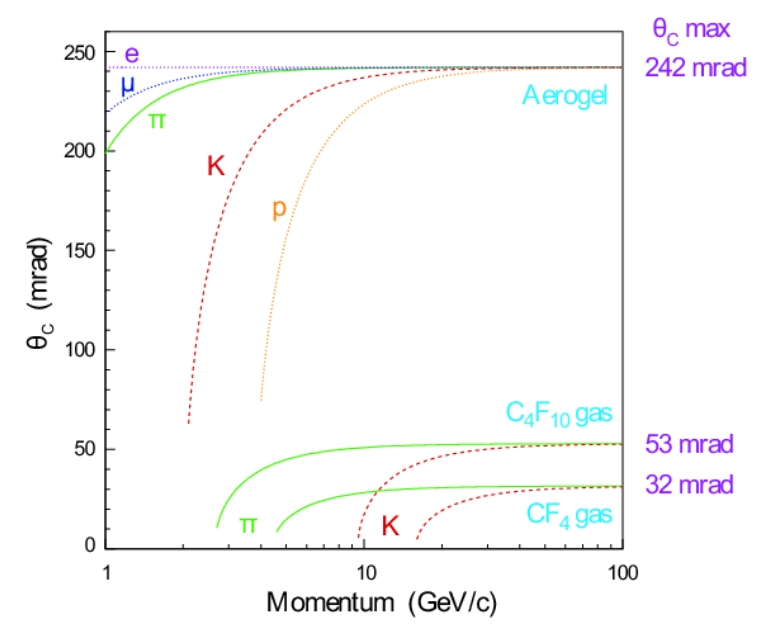
\includegraphics[width=0.55\textwidth]{richrad.jpg}
  \vspace*{-0.8cm}
  \end{center}
  \caption{\textit{Cherenkov angle versus the particle momentum for different particles in the \rich radiators.}\cite{rich}}
  \label{fig:richrad}
  \vspace*{-0.5cm}
\end{figure}

\subsubsection{The calorimeter system}
The \lhcb calorimeter system \cite{calo} consists of a Preshower detector (\presh), a Scintillating Pad Detector (\spd), an electromagnetic calorimeter (\ecal) and a hadronic calorimeter (\hcal). The main purpose of the calorimeter system is the identification of light particles such as electrons and neutral particles such as photons or \piz as illustrated in Figure \ref{fig:pid} \cite{pidcalo} and the measurement of energy and position of neutral particles that can't be detected by the tracking system. The calorimeters also provide information for the hardware based \lone trigger (see Section \ref{sec:l0}).
\begin{figure}[ht]
\vspace{-0.3cm}
  \begin{center}
    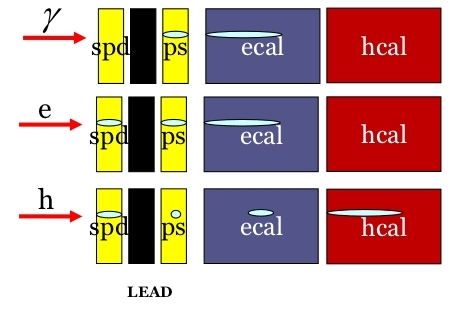
\includegraphics[width=0.5\textwidth]{CAL.jpg}
  \end{center}
  \vspace*{-1cm}
  \caption{\textit{Schematic illustration of the particle separation using the calorimeter system. The lead layer between the Scintillation Pad Detector (\spd) and the PreShower detector (\presh) is thick enough to induce electromagnetic showers.}\cite{calo}}
  \label{fig:pid}
  \vspace*{-0.5cm}
\end{figure}
% but too thin to start a significant hadronic shower

Each subdetector of the calorimeter system is composed of square cells varying in size according to the particle flux. For the \spd, \presh and the \ecal three different zones were chosen with cell sizes of $4\cm$, $6\cm$ and $12\cm$ as shown in Figure \ref{fig:calo}. The \hcal is segmented into two zones with larger cells ($13.13\cm$ in the inner section and $26.26\cm$ in the outer section) because of the size of hadronic showers. All calorimeters implement the technology of scintillation light that is transmitted to Photo-Multipliers (PMT) by wavelength-shifting (WLS) fibres.\\
\begin{figure}[ht]
  \begin{center}
  	\vspace*{-0.8cm}
    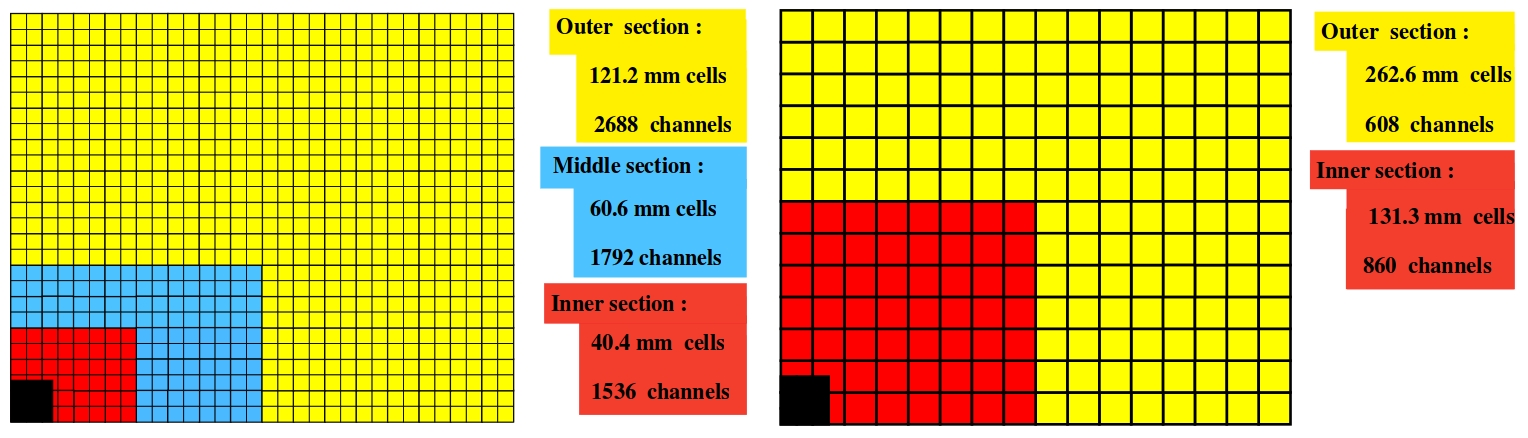
\includegraphics[width=0.85\textwidth]{calocells.jpg}
  \vspace*{-0.5cm}
  \end{center}
  \caption{\textit{Schematic illustration of the segmentation of the Scintillating Pad Detector (\spd), PreShower detector (\presh) and the \ecal (left) and the \hcal (right). The pictures show one quarter of the calorimeter surfaces. The black area on the bottom left of both images is the area close to the beam pipe where the particle flux is too high for any calorimeter performance.}\cite{calo}}
  \label{fig:calo}
  \vspace*{-0.5cm}
\end{figure}

The \presh and the \spd are located before the \ecal and separated by lead sheet of $2.5 \, \Xrad$ thickness allowing for a separation of electrons from a high background of pions. Both \presh and \spd are made of one single layer of $15\mm$ thick plastic-scintillator tiles.\\
The \ecal is composed of cells that are build after the shashlik  principle, one cell is composed of alternating layers of $2\mm$ thick lead and $4\mm$ thick polystyrene scintillator tiles. One cell, made out of 66 lead and scintillator layers, is illustrated in Figure \ref{fig:calos}.
The \hcal employs a non-typical structure where the scintillating tiles are arranged parallel to the beam pipe as shown in Figure \ref{fig:calos}. The absorber for the \hcal was chosen to be $1\cm$ iron tiles and the scintillator layers are made out of $3\mm$ thick doped polystyrene tiles.
\begin{figure}[ht]
  \vspace*{-0.5cm}
  \begin{center}
  \subfigure{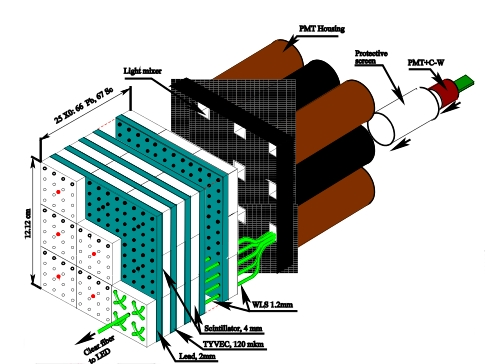
\includegraphics[width=0.45\textwidth]{ECAL.jpg}}
   \subfigure{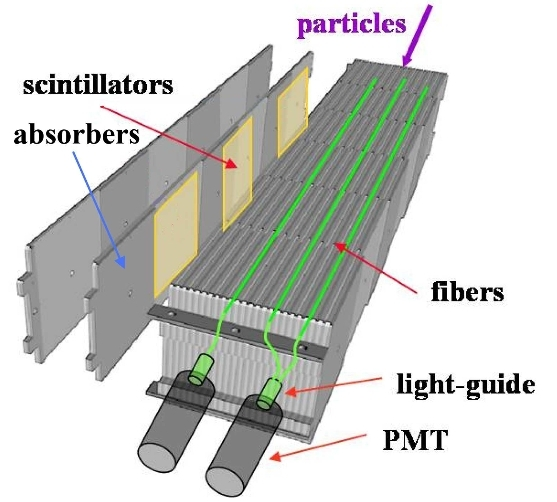
\includegraphics[width=0.43\textwidth]{hcal1.jpg}}
  \vspace*{-0.8cm}
  \end{center}
  \caption{\textit{One cell of the \ecal (left) and the \hcal (right). The scintillating tiles of the \ecal are arranged perpendicular to the beam while they are parallel to the beam for the \hcal. The absorber is made of lead for the \ecal and iron for the \hcal.}\cite{calo}}
  \label{fig:calos}
\end{figure}


\subsubsection{The muon chambers}
The \lhcb detector contains five muon stations (\Mone - \Mfive) dedicated to muon identification and muon triggering \cite{muon}.\\
The first muon station \Mone is placed upstream of the calorimeters to provide a precise transverse momentum measurement. The other muon stations are placed downstream of the calorimeters and interleaved with $80\cm$ thick iron absorbers. The stations \Mtwo and \Mthree yield a very good spacial resolution for the tracks while the last two stations only deliver information for the particle identification. The side view of the muon system is shown in Figure \ref{fig:muons}.\\
As can be seen on the left in Figure \ref{fig:muons}, each muon chamber is divided into four regions R1 to R4. The granularity in the regions decreases radially which provides an isotropic channel occupancy for each muon station. Except for the inner region R1 of \Mone, all muon stations are composed of Multi Wire Proportional Chambers (MWPC). R1 of \Mone implements the Triple GEM \cite{gem} technology because the particle flux in this region would overburden the MWPC.\\
\begin{figure}[ht]
\vspace*{-0.5cm}
  \begin{center}
  \subfigure{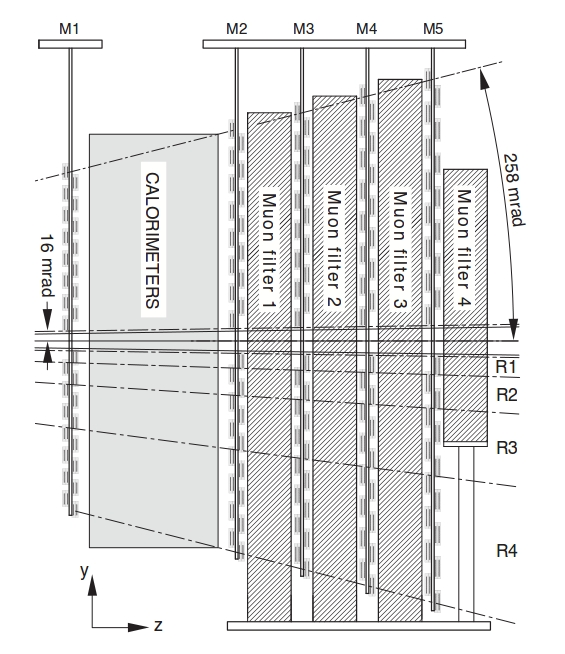
\includegraphics[width=0.35\textwidth]{muon2.jpg}}
   \subfigure{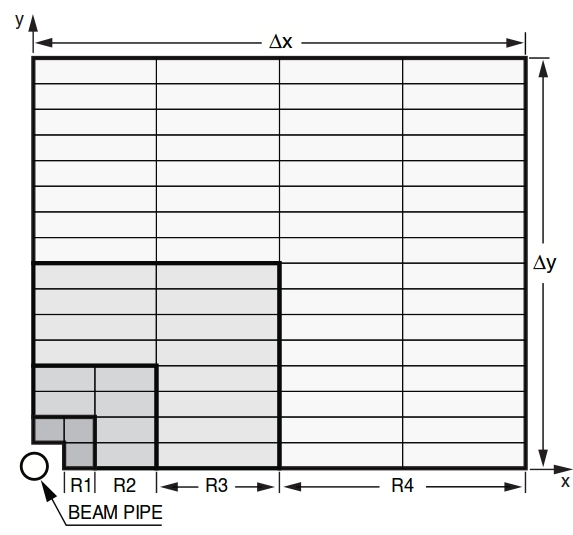
\includegraphics[width=0.35\textwidth]{muon1.jpg}}
  \vspace*{-1.0cm}
  \end{center}
  \caption{\textit{Side view of the muon stations (left) and the schematic front view of the upper right quarter of one muon station with the segmentation into four regions R1 to R4. All modules are composed of MWPC except for R1 of M1 which uses the Triple GEM technology due to extremely high particle flux.}\cite{muon}}
  \label{fig:muons}
\end{figure}

\subsubsection{The discriminant particle identification variable}
\label{sec:pid}
The information from the detectors of the particle identification system is used in the offline analysis to calculate a discriminative variable $\mathrm{DLL}$. This variable is calculated for all final state tracks. It is computed by testing the hypothesis that a track is a certain particle with respect to the hypothesis that the track comes from another particle. The reference particle is usually chosen to be a pion.\\
The information on the particle identification variable for kaons and pions (\dllkpi) comes mainly from the \richone and \richtwo. For neutral particles and electrons (\dllepi) the calorimeter system provides the significant information while the particle identification variable for muons (\dllmupi) is calculated by relying especially on the muons system.\\

\subsection{\lhcb performance summary}
The \lhcb detector has shown a high and stable performance over the entire range of data taking \cite{lhcbperf}.\\
%The primary vertex resolution obtained by the \velo is $13 \mum$ for the $x$ and $y$ coordinates and $69 \mum$ for the $z$ coordinate for an average of $25$ tracks coming from the primary vertex \cite{veloperf} \cite{tsperf}. An equally excellent impact parameter resolution of $<35 \mum$ for tracks with a transverse momentum $p_T>1 \gev$ can be obtained. The resolution of the $x$ and $y$ coordinates of the primary vertex and the resolution on the impact parameter's $x$ coordinate are shown in Figure \ref{fig:resolution}. 
%The \lhcb tracking system has an average relative momentum resolution of $0.5 \%$. \\
The resolution of the $x$ and $y$ coordinates of the primary vertex and the resolution on the impact parameter's $x$ coordinate are shown in Figure \ref{fig:resolution}. For 25 tracks a resolution of $13 \mum$ on the $x$ and $y$ coordinates and a resolution of $69 \mum$ on the $z$ coordinate of the primary vertex can be reached \cite{veloperf}. Additionally an equally excellent impact parameter resolution of $<35 \mum$ for tracks with a transverse momentum $p_T>1 \gev$ can be obtained. The tracking system has an average relative momentum resolution of
\begin{equation}
\frac{\Delta p}{p} = 0.5 \% \quad \cite{tsperf}.
\end{equation}
The relative energy resolution for the \ecal is
\begin{equation}
\frac{\Delta E}{E} = \frac{10 \%}{\sqrt{E[\gevc]}} \oplus 1\%
\end{equation}
and for the \hcal
\begin{equation}
\frac{\Delta E}{E} = \frac{80 \%}{\sqrt{E[\gevc]}} \oplus 10\%
\end{equation}
\\
The particle identification system has varying performances for different particle types and momenta. For example, the average electron identification efficiency is $90\%$ for a $5\%$ misidentification rate. The average kaon identification efficiency is $95\%$ for a $5\%$ rate of misidentifying a pion as a kaon.
\begin{figure}[ht]
  \begin{center}
  \subfigure{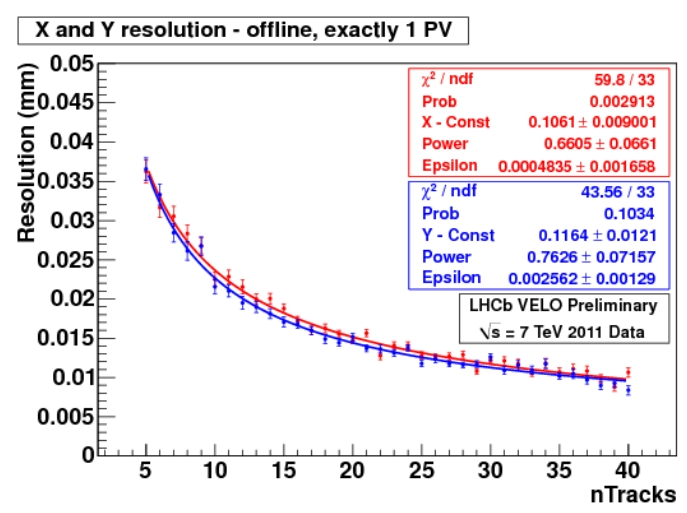
\includegraphics[width=0.49\textwidth]{PVresolution.jpg}}
    \subfigure{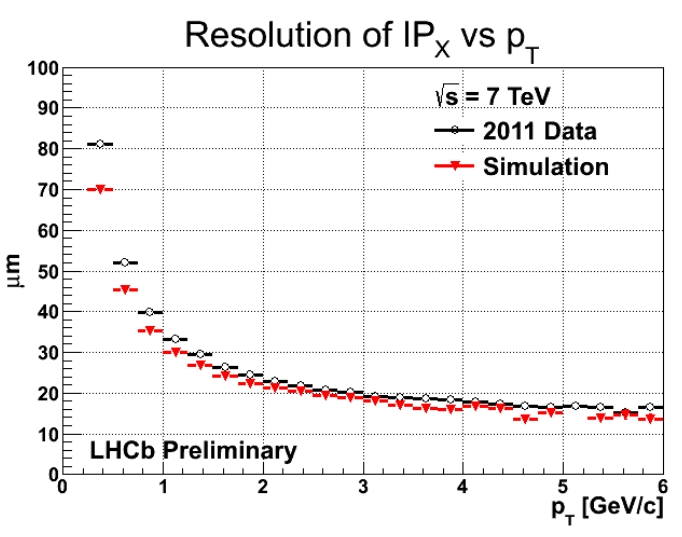
\includegraphics[width=0.49\textwidth]{IPresolution.jpg}}
  \vspace*{-1.0cm}
  \end{center}
  \caption{\textit{Summary of the performance of \lhcb tracking system obtained from 2011 data and Monte Carlo. The primary vertex resolution for the $x$ and $y$ coordinates as a function of the number of tracks (left) and the of the $x$ coordinate of the impact parameter as a function of the transverse momentum $p_T$.}\cite{veloperf}}
  \label{fig:resolution}
\end{figure}
\newpage
%
%
%
\vspace{0.5cm}
\section{The trigger system}
The \lhc collides bunches at a rate of $40 \mhz$. Due to the \lhcb's luminosity levelling the visible\footnote{To be visible, events must have at least two charged particles producing enough hits in the tracking system to be reconstructed.} rate of interaction is $10\mhz$ which has to be reduced to about $4\khz$ to be permanently stored for offline analysis. At \lhcb this is realized by a two-stage trigger system \cite{trigger} \cite{trigger2}: the Level-0 (\lone), a purely hardware based trigger, followed by the High Level Trigger (\hlt) which is executed on a processor farm. A schematic presentation of the trigger system can be seen in in Figure \ref{fig:trigger}.
\begin{figure}[ht]
\vspace*{-0.3cm}
  \begin{center}
    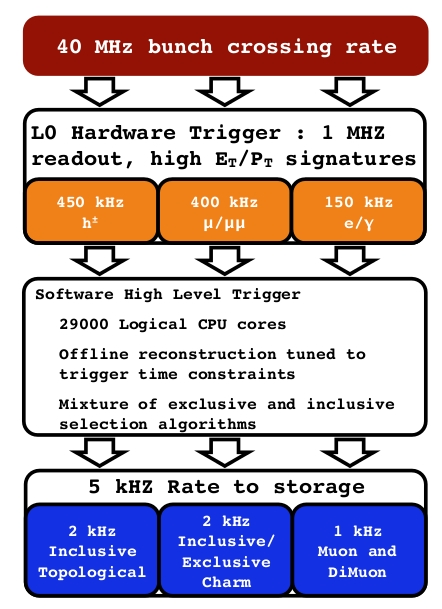
\includegraphics[width=0.43\textwidth]{trigger.jpg}
  \vspace*{-0.5cm}
  \end{center}
  \caption{\textit{A schematic representation of the \lhcb trigger system. The first state is the hardware based Level-0 trigger. Afterwards the High Level Triggers are executed on a processor farm. Each subtrigger uses several trigger lines for dynamic and specific triggering.}}
  \label{fig:trigger}
\end{figure}


\subsection{The Level-0 trigger}
\label{sec:l0}
The \lhcb Level-0 (\lone) trigger is made from custom electronics and reduces the rate from $10\mhz$ to $1\mhz$.\\
To identify events from \B hadrons the \lone trigger makes use of the fact that the large mass of \B hadrons provides a significant amount of transverse kinetic energy to the decay particles. Therefore it selects events with a high amount of transverse energy deposited in the calorimeter or the muon system. Additionally, the \lone accesses information from the \velo pileup and the \spd to reject events with too many tracks. There are different \lone trigger lines for different particles. The two lines important for the analysis are the \lone Electron and the \lone Hadron which will be presented in the following.\\
% Within the bandwidth allocated to the electron trigger (cf. section 7.1.2) the electron Level 0 trigger is required to reject 99\% of the inelastic pp interactions while providing an enrichment factor of at least 15 in b events. This is accomplished through the selection of electrons of large transverse energy ET.  and the \lone TIS (Trigger Independent of Signal)
\newpage
\textbf{The \lone Electron} trigger line is fired by one electromagnetic cluster ($2\times 2$ \ecal cells) with a transverse energy $E_T$ above a threshold value. The electromagnetic cluster must have at least one corresponding hit in the \spd to identify a charged particle opposed to a photon. The threshold value for the transverse energy of the electromagnetic cluster has changed several times over the years 2011 and 2012. This will be evaluated further in Chapter \ref{Chapter4} in Section \ref{sec:triggercat}.\\
\textbf{The \lone Hadron} trigger line is activated by one cluster in the \hcal. The threshold transverse energy $E_T$ for the \lone Hadron is the sum of the transverse energy in the \hcal with the transverse energy the corresponding \ecal cells.
\\
\subsection{The High Level Trigger}
\label{sec:hlt}
All events that pass the \lone trigger will be passed on to the High Level Trigger (\hlt). The \hlt is divided into two levels (\hltone and \hlttwo) which are both implemented as a set of \cpp algorithms run on a CPU farm.\\
\\
Additionally to the information available to the \lone, the \hltone has access to information from the \velo and the tracking system. It reconstructs particles in the \velo and determines the position of the primary vertices in each event. The \hltone then makes a decision based upon impact parameter, momentum, transverse momentum and/or track quality of one track in the event.\\
For each \lone line several \hltone lines are executed. The \hltone reduces the rate to approximately $40 \khz$.\\
\\
All events that pass the \hltone go through to the \hlttwo that performs an event reconstruction similar to the offline analysis. Starting by reconstructing all tracks in the event using the \velo tracks as seed, the \hlttwo reconstructs intermediate particles and resonances and identifies displaced vertices. Afterwards, depending on the \hlttwo line, different sets of selections are applied which are dominantly designed to identify decays of \B and \D hadrons. The \hlttwo finally reduces the rate to about $4\khz$ which is stored for the offline analysis.\\
\\
One \hltone line and several \hlttwo lines will be used in the analysis of the\\ \BdKstee decay. The \hltone line that is used, is the  \textit{Hlt1TrackAllL0Decision} line. This line selects events with at least one track with a high transverse momentum $p_T$ and a great impact parameter (IP) with respect to the primary vertex, since this track is likely to come from a decaying \B hadron.\\
The \hlttwo lines that are used are the \textit{\hlttwo topological lines} \cite{hlt2topo}. These have been designed to trigger inclusive $n$-body ($n = 2,3,4$) \B decays. The \hlttwo lines implement a $Boosted Decision Tree$ to determine if $n$ tracks show the topology of a \B decay. Missed tracks are compensated for by tacking into account the difference between the total momentum of the $n$ tracks and the momentum of the hypothetical \B hadron.\\
\newpage

\section{The \lhcb stripping}
In order to reduce computing time, all events are preselected by a certain \textit{stripping line}. A stripping line consists of a loose selection aiming at rejecting as much background as possible while keeping as much signal as possible. Each decay studied at \lhcb has its own stripping line. All stripping lines are run on the entire dataset regardless of the trigger decision. The stripping is executed by the physics analysis software \davinci (see Section \ref{sec:software}).\\
During the stripping procedure every event is scanned for tracks that can be combined (see Chapter \ref{chapter3}) to make the signal decay. Events with signal candidates are stored for later use.\\

\section{The \lhcb software}
\label{sec:software}
The data processing at \lhcb goes through a series of steps which are executed by different software frameworks. To ensure consistency between these frameworks and the way that data and Monte Carlo are treated, all \lhcb core software is embedded in the \gaudi framework \cite{gaudi}.\\
There are four main applications, each responsible for a different stage of event processing:
\\
\begin{itemize}
\item \textbf{\gauss}is used for the generation of Monte Carlo. Therein, proton-proton collisions are simulated with \pythia \cite{pythia}, the decay of \B hadrons is made with \evtgen \cite{evtgen} and the detector simulation is implemented in \geant \cite{geant}.\\
\item \textbf{\boole}takes the output from \gauss and simulates the digitization of data to give it the same format as the \lhcb data obtained by the electronics and data acquisition systems.\\
\item \textbf{\brunel}performs subdetector and global reconstruction using pattern recognition for both Monte Carlo and real data.\\
\item \textbf{\davinci}executes the last step, namely the reconstruction of the final signal events and running the stripping \cite{davinci}(more details in Chapter \ref{chapter3}).
\end{itemize}

%\textbf{The \lone TIS trigger line}
%All decays that were not triggered by one of their own tracks but later on selected by the Stripping (see Section \ref{sec:stripping}) are called TIS events because the events was triggered independently from the signal by another track in the events, coming from the other \B hadron for example. The \lone TIS decays are most free from any trigger systematics and the trigger efficiency is independent of the decay which is absolutely not the case for the other trigger lines.\\
%\chapter{Study of the reconstruction of the \BdKstee invariant mass}
\chaptermark{Chapter4}
\label{chapter3}
%\addcontentsline{toc}{chapter}{Study of the reconstruction of the \BdKstee invariant mass}
The event reconstruction is a crucial part of the analysis of any decay. At \lhcb, the offline event reconstruction is made in two steps. The first step is executed by the software \brunel that performs subdetector and global reconstruction using pattern recognition for both Monte Carlo and real data. \brunel takes the detector information and reconstructs \textit{tracks} from the hits. The information for each \textit{track} is then stored for further analysis.\\
The second step, the one accessible and adjustable by every user, is executed by the \davinci physics and analysis framework. At the beginning of every event reconstruction \davinci builds lists of \textit{particles}. For each particle-type, such as electron or kaon, there are several lists ranging from very loose to very tight requirements on the \textit{tracks}. For each list, \davinci selects all the \textit{tracks} provided by \brunel that fulfil the list conditions and fully reconstructs them as \textit{particles}, quantities of physics with a four-momentum. In the course of this reconstruction the mass of the \textit{particle} is fixed to the particle-type's mass defined by the list.
%These \textit{particles} are made from the \textit{track} information provided by \brunel and are quantities of physics with a four-momentum. In the course of computing the \textit{particles} properties their masses are fixed to the value corresponding to the condition of the list, e.g. all particles in the list \textsc{SdtAllLooseKaons} have a mass of $493 \mevcc$.\\
From the lists of \textit{particles} \davinci reconstructs intermediate particles (e.g. \Kstarz from \Kp and \pim) and finally the entire \BdKstee decay. \davinci allows the user to choose the \textit{particle} lists and the algorithms that compute their properties, additionally to the way the \textit{particles} are being combined.\\ % einfuegen von bezug auf arbeit
\\
The greatest difficulty in reconstructing the \BdKstee decays is the measurement of the electron\footnote{Throughout this chapter electron stands for electrons and positrons if not mentioned otherwise.} energy. This difficulty arises from bremsstrahlung radiation and propagates to a vast degradation of the \Bd mass resolution. The effects occurring due to bremsstrahlung of the electrons and the means of limiting the loss in precision -- namely different event reconstruction tools implemented in the \davinci framework -- are presented in the following Section. \\
In Section \ref{sec:DiElectronMaker} the focus is put on the reconstruction on the invariant mass of the electron pair $M_{inv}(\epem)$.\\
\newpage
\section{Bremsstrahlung radiation}
\label{sec:bremsstrahlung}
When traversing the material of the detector charged particles undergo a probability of emitting bremsstrahlung. The cross-section for bremsstrahlung emission $\sigma_{bs}$ is anti-proportional to the square of the charged particle's mass $m$ \cite{WRLeo}.
\begin{equation}
 d\sigma_{bs} \propto \frac{e^2}{(mc^2)^2}
\end{equation}
Since the amount of material is low in \lhcb the probability of emitting bremsstrahlung photons is negligible for heavier particles, but very light particles such as electrons and positrons can lose a significant amount of energy through bremsstrahlung radiation. The amount of energy emitted through bremsstrahlung for muons $E_{bs}^{\mmu}$ for instance, is suppressed by a factor $40\ 000$ with respect to that of electrons $E_{bs}^{\electron}$.
\begin{equation}
\frac{E_{bs}^{\electron}}{E_{bs}^{\mmu}} = \frac{m_{\electron}^2}{m_{\mmu}^2} = 2.3 \cdot 10^{-5} 
\label{eq:evsmu}
\end{equation}
%At energies below a few \gev only electrons emit a significant amount of bremsstrahlung radiation in the \lhcb detector.\\
The radiated energy spectrum for the electrons from \BdKstee before the \lhcb magnet is shown in Figure \ref{fig:totalEnergyLossBrems}. The distribution was obtained by performing a Fast-Sim \cite{ananote} on Monte Carlo at simulation level under the assumption of complete screening \cite{pdg}.
\begin{figure}[ht]
  \begin{center}
    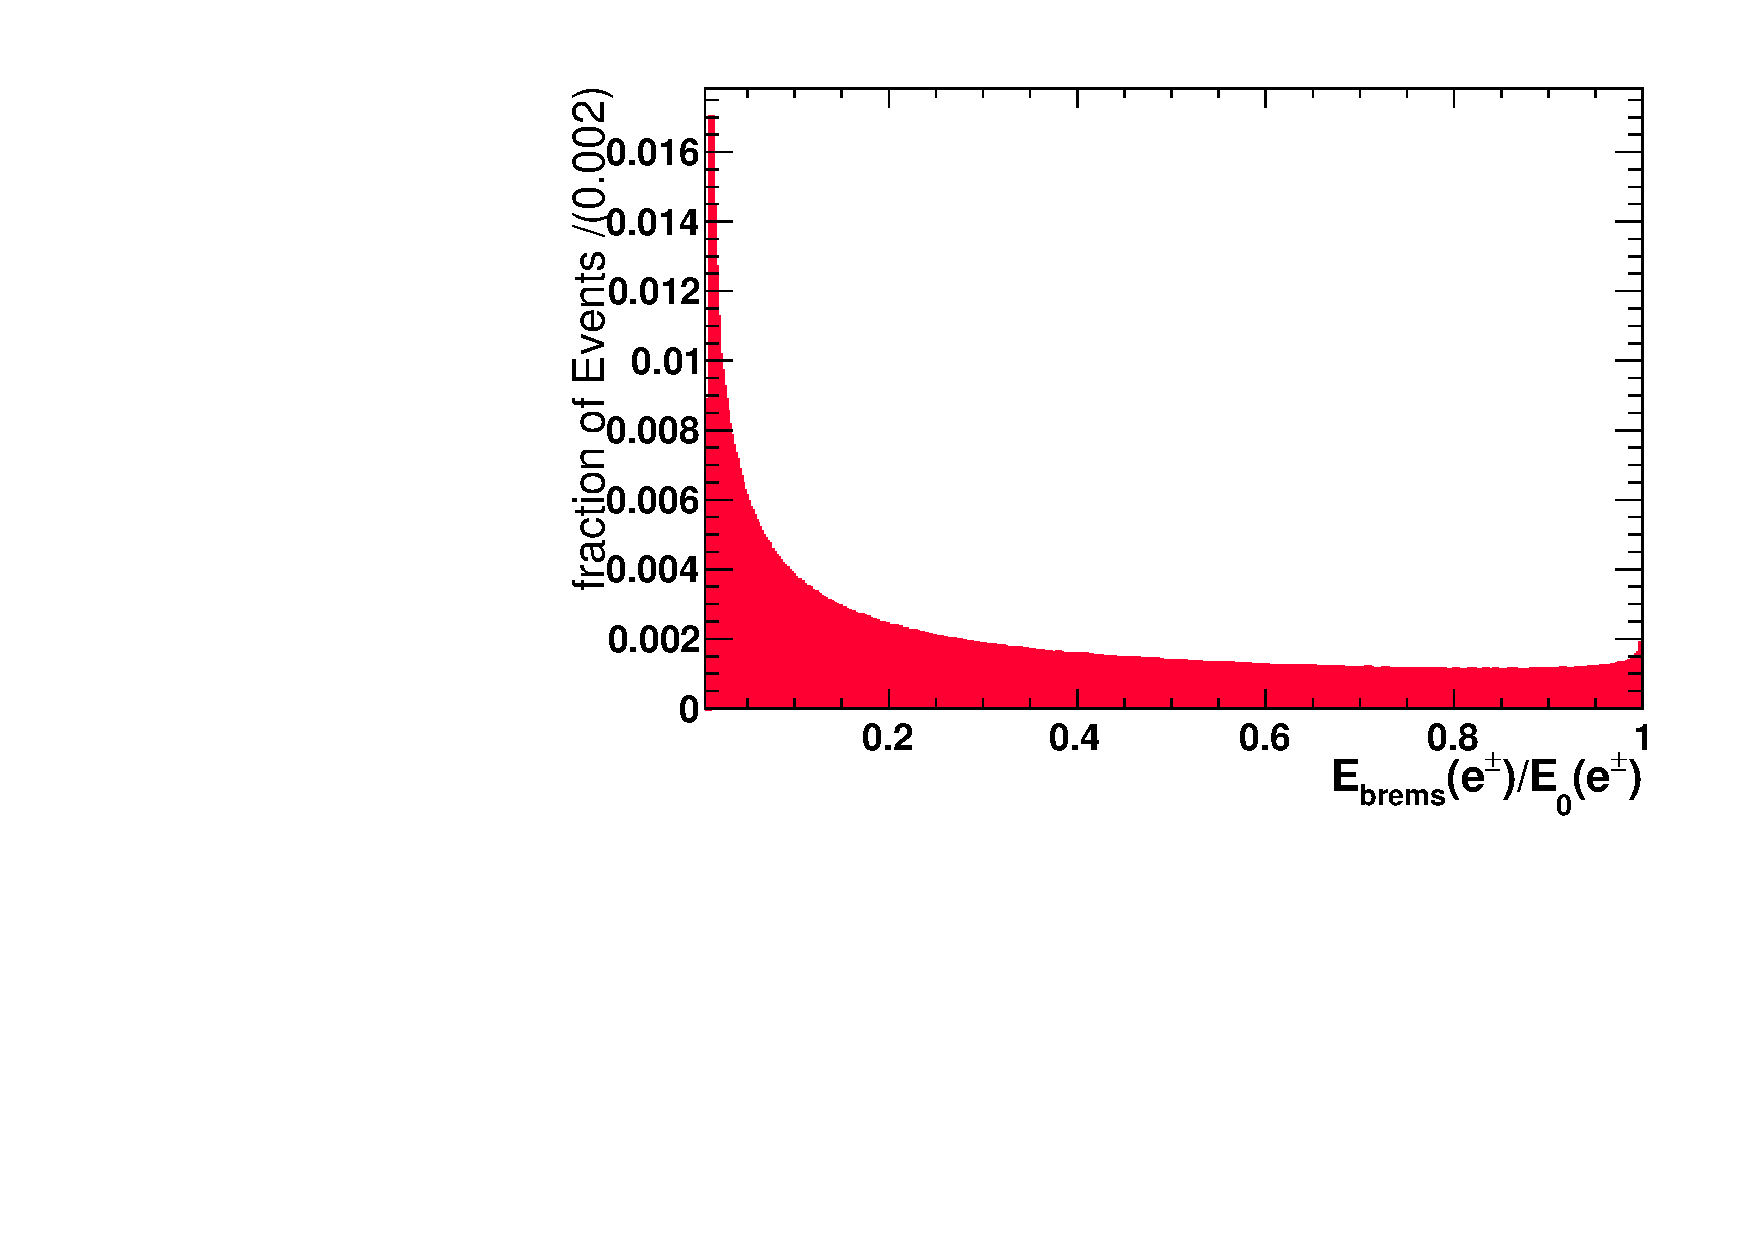
\includegraphics[width = 0.55\textwidth]{EnergyLossBrems.pdf}
    \end{center}
    	\vspace*{-0.8cm}
  \caption{\textit{Percentage of energy loss of electrons/positrons traversing the \lhcb detector before the magnet. $E_{brems}(\epm)$ denotes the energy radiated by the electron/ positron while $E_0(\epm)$ stands for the initial electron/positron energy. Distribution obtained by performing a Fast-Sim on Monte Carlo Data at simulation level under the assumption of complete screening.}}
  \label{fig:totalEnergyLossBrems}
\end{figure}

The bremsstrahlung radiation process is of statistical nature. Figure \ref{fig:totalEnergyLossBrems} shows the amount of radiated energy. It is therefore crucial to identify photons in the detector that have been emitted by electrons through bremsstrahlung radiation and add their four-momentum to the four-momentum of the electron track. The \Bd mass distribution without any kind of bremsstrahlung reconstruction can be seen in Figure \ref{fig:noBremReco}.
\newpage
\begin{figure}[ht]
  	\centering
    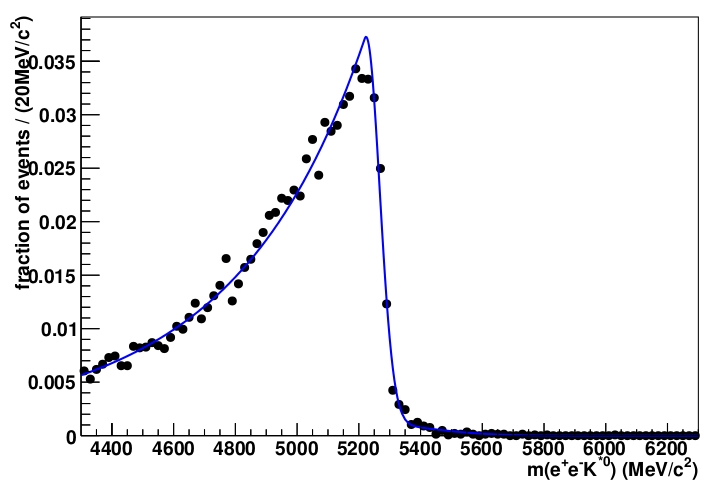
\includegraphics[width = 0.55 \textwidth]{oldBrem_noBremReco.jpg}
  \caption{\textit{The \Bd mass distribution of \BdKstee \lhcb Monte Carlo without any reconstruction of bremsstrahlungs photons.}}
  \label{fig:noBremReco}
\end{figure}

\subsection{Bremsstrahlung recovery}
\label{sec:bremsstrahlungrecovery}
If the emission of the bremsstrahlung happens before the magnet, the electron will be deflected from its initial trajectory by the magnetic field while the bremsstrahlung photon's momentum will not change, as shown in Figure \ref{fig:bremsstrahlung}. Thus, the electron and its photon will deposit their energies in different positions in the \ecal. To allow nonetheless for an assignment of the bremsstrahlung photon with its electron \textit{bremsstrahlung recovery algorithms} have been developed. These algorithms search for bremsstrahlung photon candidates in the \ecal and try to match them to the corresponding electron track.Two different bremsstrahlung recovery algorithms implemented in the \lhcb physics analysis framework will be presented in Sections \ref{sub:oldBrem} and \ref{sub:newBrem}.
\begin{figure}[ht]
\vspace*{-0.4cm}
  \begin{center}
    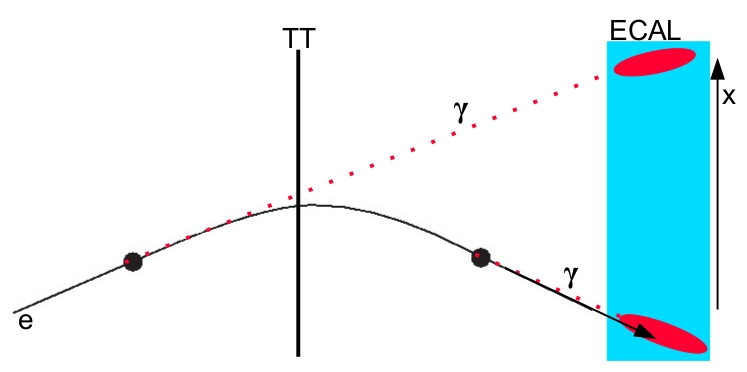
\includegraphics[width=0.6\textwidth]{BremReco.jpg}
  \end{center}
  \vspace*{-0.5cm}
  \caption{\textit{Schematic illustration of bremsstrahlung emission of electrons in the \lhcb detector.}}
  \label{fig:bremsstrahlung}
\end{figure}
If the emission of the bremsstrahlung happens after the magnet, the electron and its photon will deposit their energies in the same \ecal cells. Thus the photon energy is automatically added to the energy of its electron. \\


\subsubsection{Bremsstrahlung recovery algorithm in \davinci v29 }
\label{sub:oldBrem}
The first bremsstrahlung recovery tool was the standard algorithm implemented in all version of \davinci up to v29. An illustration of its methodology is shown in Figure \ref{fig:oldBremAdd}.
\begin{figure}[ht]
\vspace*{-0.5cm}
  \begin{center}
  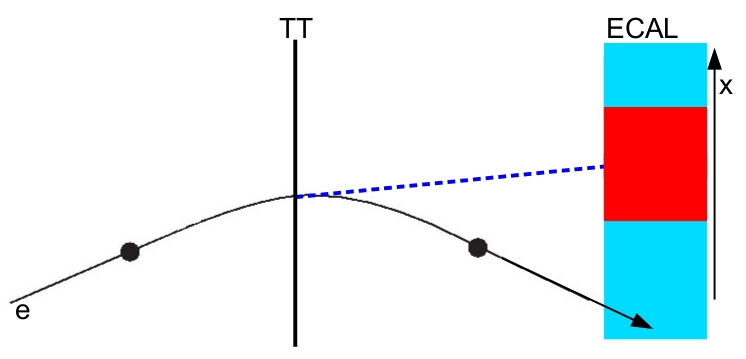
\includegraphics[width=0.6\textwidth]{oldBremAdder.jpg}
  \end{center}
  \vspace*{-0.5cm}
  \caption{\textit{Schematic illustration of the bremsstrahlung recovery algorithm \davinci v29. Black line: curve of the electron track. Dark blue dotted line: linear extrapolation of the electron track from its very first state to the \ecal. Clear blue dotted line: linear extrapolation of the electron track from its last state before the magnet to the \ecal. Red area in the \ecal: area from where photon candidates will be matched to the electron track.}}
  \label{fig:oldBremAdd}
\end{figure}
The algorithm starts with a \textit{particle} list of electrons and searches for reconstructed photon candidates coming from the electron tracks.
To predict the position of bremsstrahlung photon candidates in the \ecal, the algorithm linearly extrapolates the electron track from the \ttracker (last state before the magnet) to the \ecal. All neutral clusters in the \ecal whose barycentric positions match the position of the extrapolated electron track with a $\chi^2 < 300$ are accepted as bremsstrahlung photons. Their four-momentum is added to the four-momentum of the electron. Furthermore there is no limit of bremsstrahlung photon candidates that can be added to one electron.\\


\subsubsection{Bremsstrahlung recovery algorithm in \davinci v30}
\label{sub:newBrem}
The second bremsstrahlung recovery tool is implemented in \davinci v30. Its methodology is illustrated in Figure \ref{fig:newBremAdd}.
\begin{figure}[ht]
  \begin{center}
  \label{fig:newBremAdder}
  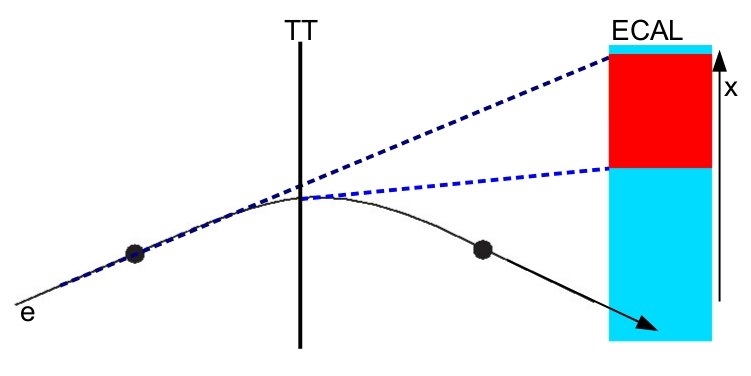
\includegraphics[width=0.6\textwidth]{newBremAdder.jpg}
  \end{center}
  \vspace{-0.8cm}
  \caption{\textit{Schematic illustration of the bremsstrahlung recovery algorithm \davinci v30. Black line: curve of the electron track. Dark blue dotted line: linear extrapolation of the electron track from its very first state to the \ecal. Clear blue dotted line: linear extrapolation of the electron track from its last state before the magnet to the \ecal. Red area in the \ecal: area from where photon candidates will be matched to the electron track.}}
  \label{fig:newBremAdd}
\end{figure}
For each \textit{particle} in the electron list two linear extrapolations of the track are computed, namely the extrapolation of the electron track from its very first state in the \velo to the \ecal and from its state in the \ttracker to the \ecal. Photon candidates must satisfy tighter conditions than for the algorithm in \davinci v29 \footnote{Photon candidates for the \davinci v30 bremsstrahlung recovery algorithm must satisfy the conditions of a PhotonID greater than $-0.5$ and a $p_T$ greater than $75 \mevc$.}.
The $x$ position of the photon candidates in the \ecal must lie between the $x$ positions of the two electron track extrapolations within $\pm 2 \sigma_{x}$. The $y$ position of the photon candidate in the \ecal must match the $y$ position of the electron track extrapolations within $\pm 2 \sigma_{y}$. The $\sigma_{x,y}$ denote the square root of the quadratic sum of the photon cluster spread with the error on the electron track extrapolations. \\



\subsection{The mechanism of double counting}
\label{sec:doublecounting}
Both bremsstrahlung recovery algorithms implemented in \davinci have the disadvantage of generating \textit{double counting}. Double counting occurs when one bremsstrahlung photon candidate can be associated to more than one electron track. This happens particularly often for the \BdKstee decay mode where the $e^+e^-$ invariant mass is very low, yielding small angles between the electron and the positron, as is illustrated in Figure \ref{fig:schemdc}. The distribution of double counting events depending on the $M_{inv}(e^+e^-)$ is shown in Figure \ref{fig:Minveedouble counting}. In the case of double counting the bremsstrahlung recovery algorithms add the photon's four momentum to both the electron's and the positron's four momentum. In the case of \BdKstee, these events will show a non-physically high $B^0$ mass and lead to a non-typical symmetric \Bd mass distribution that can be seen in Figure \ref{fig:oldBremAddernodcc}. 
\begin{figure}[ht]
\vspace*{-0.5cm}
  \begin{center}
  \label{fig:newBremAdder}
  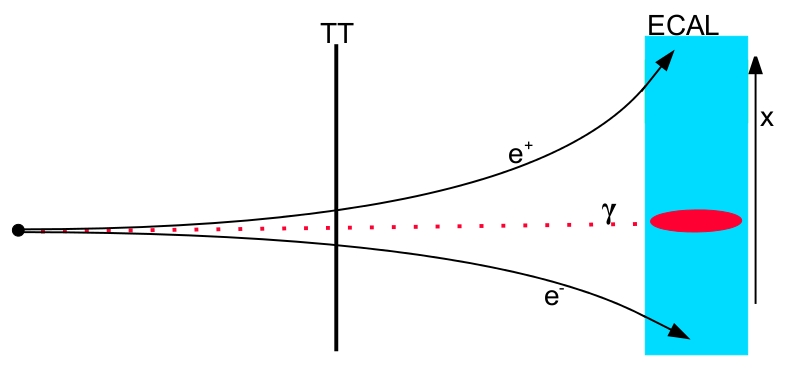
\includegraphics[width=0.6\textwidth]{doublecounting.jpg}
  \end{center}
  \vspace*{-0.5cm}
  \caption{\textit{Schematic illustration of the mechanism of double counting. Due to a very low $e^+e^-$ invariant mass the angle between the electron and the positron is so small that the photon can be associated to both.}}
  \label{fig:schemdc}
  \vspace*{-0.5cm}
\end{figure}

\begin{figure}[ht]
  \begin{center}
  \vspace*{-.6cm}
  \subfigure{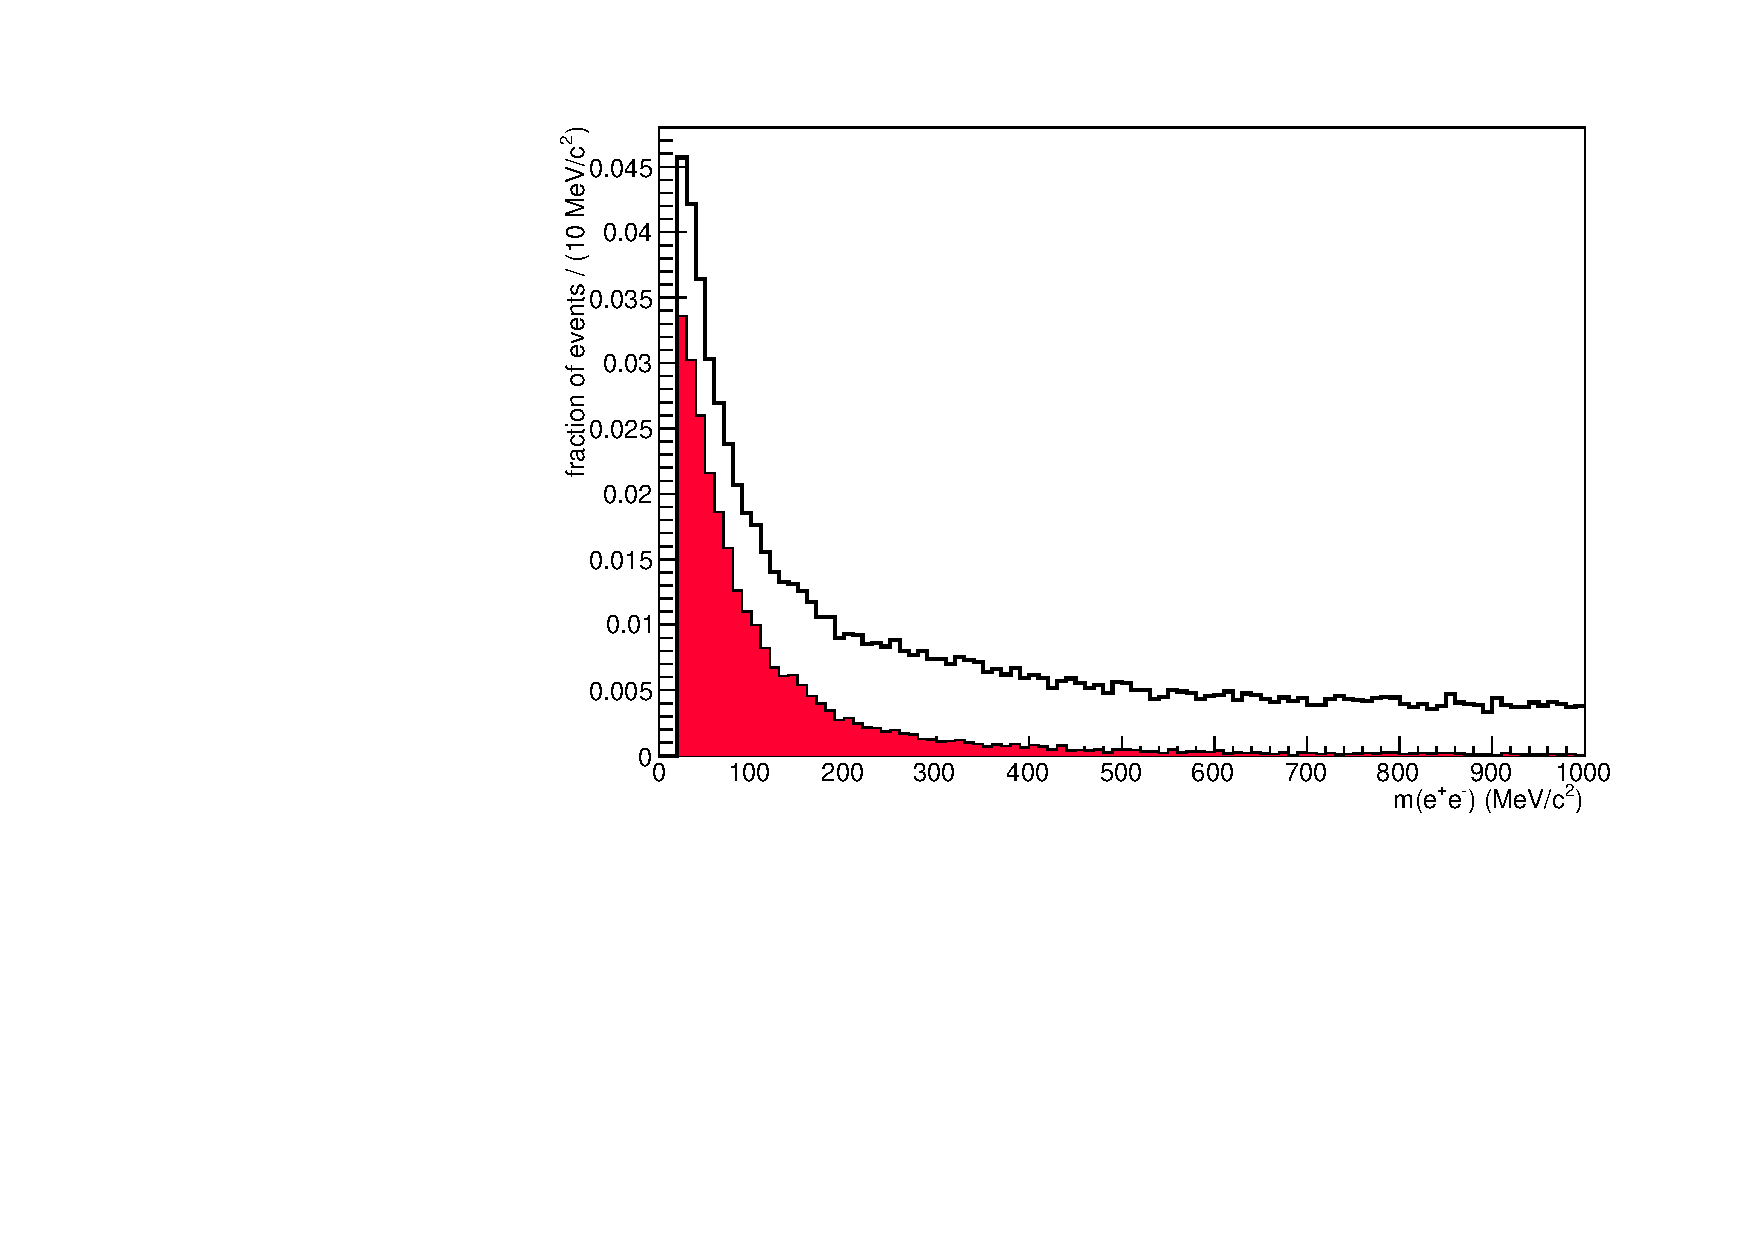
\includegraphics[width=0.48\textwidth]{dccats_Minvee_oldBrem.pdf}}
    \subfigure{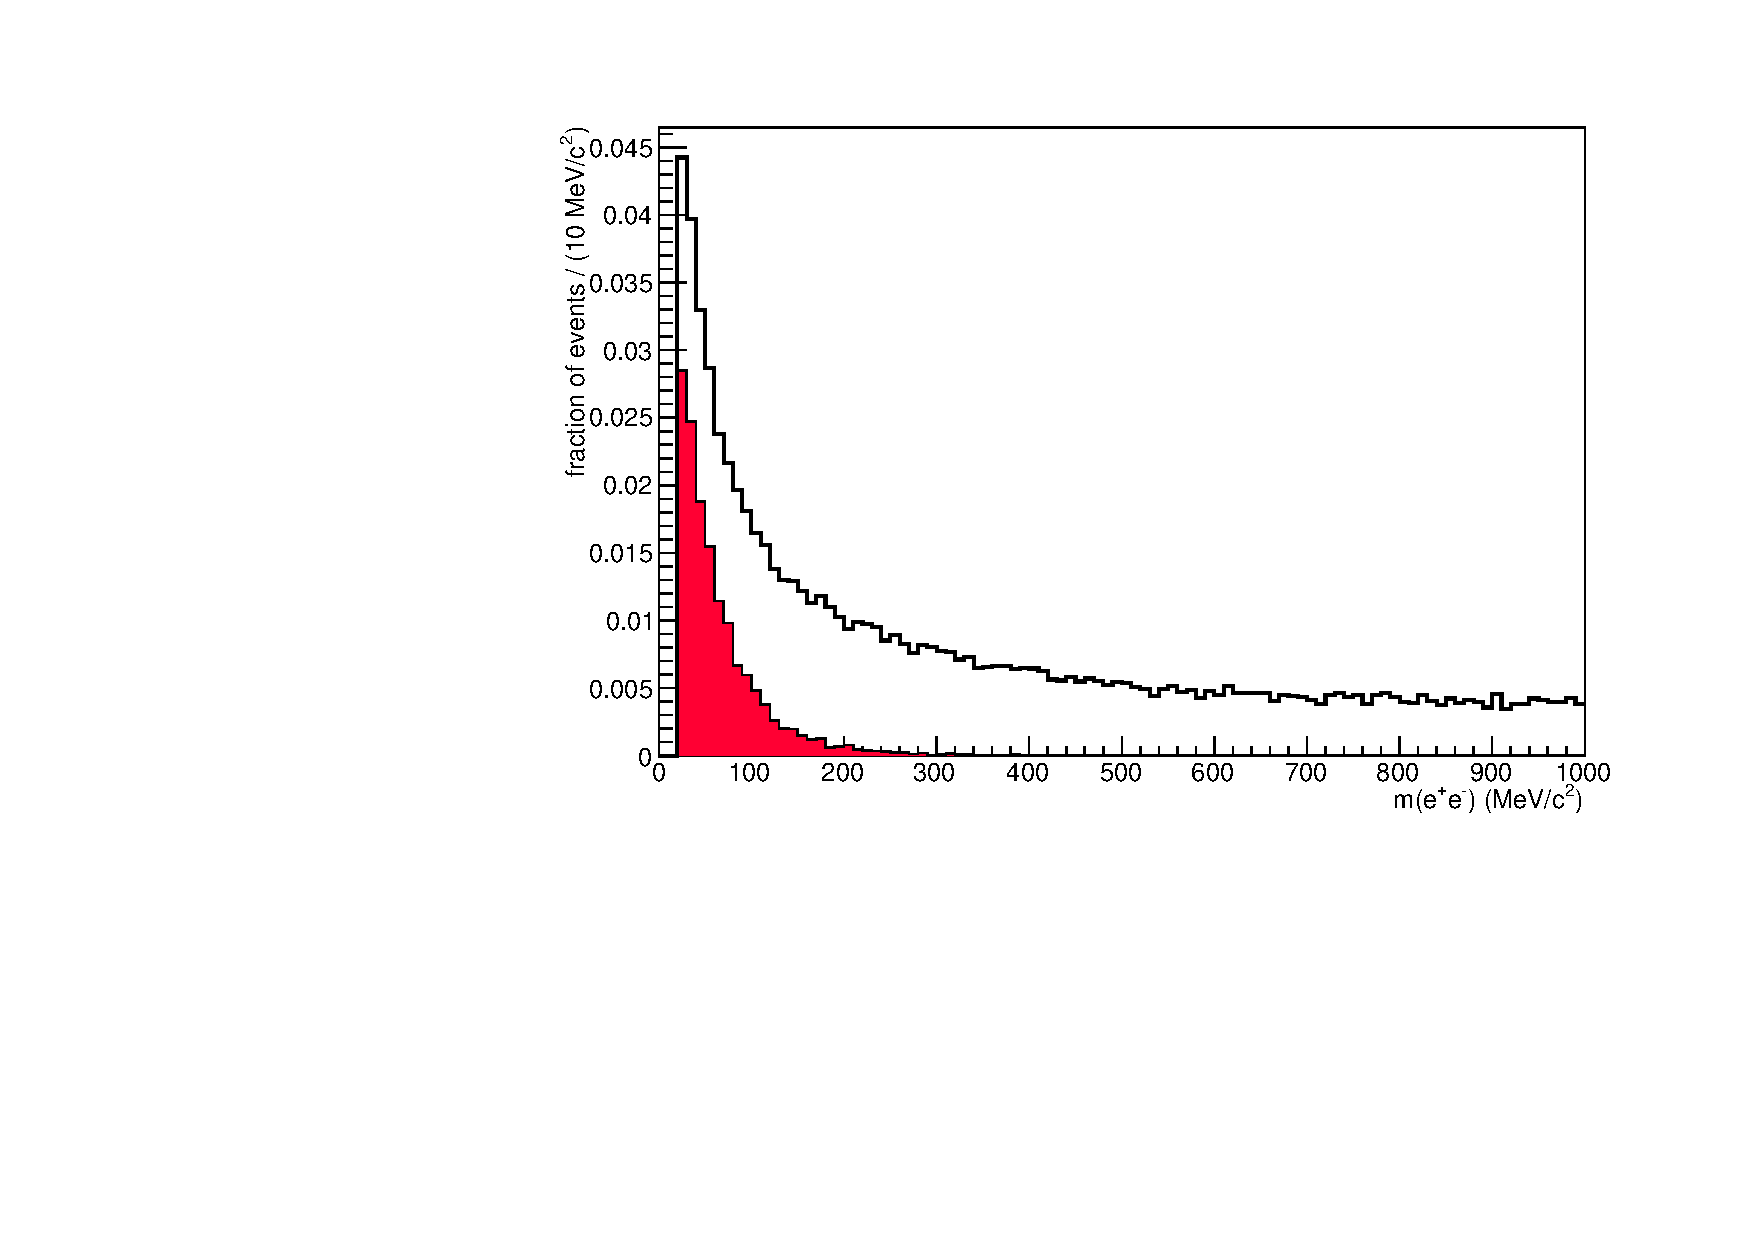
\includegraphics[width=0.48\textwidth]{dccats_Minvee_newBrem.pdf}}
  \vspace*{-1.0cm}
  \end{center}
  \caption{\textit{$M_{inv}(e^+e^-)$ distribution obtained by reconstructing \lhcb Monte Carlo with \davinci v29 (left) and \davinci v30 (right) respectively.. The pink distribution are the events with double counting.}}
  \label{fig:Minveedouble counting}
  \vspace*{-0.5cm}
\end{figure}


\begin{figure}[ht]
\vspace*{-0.5cm}
  \begin{center}
  \subfigure{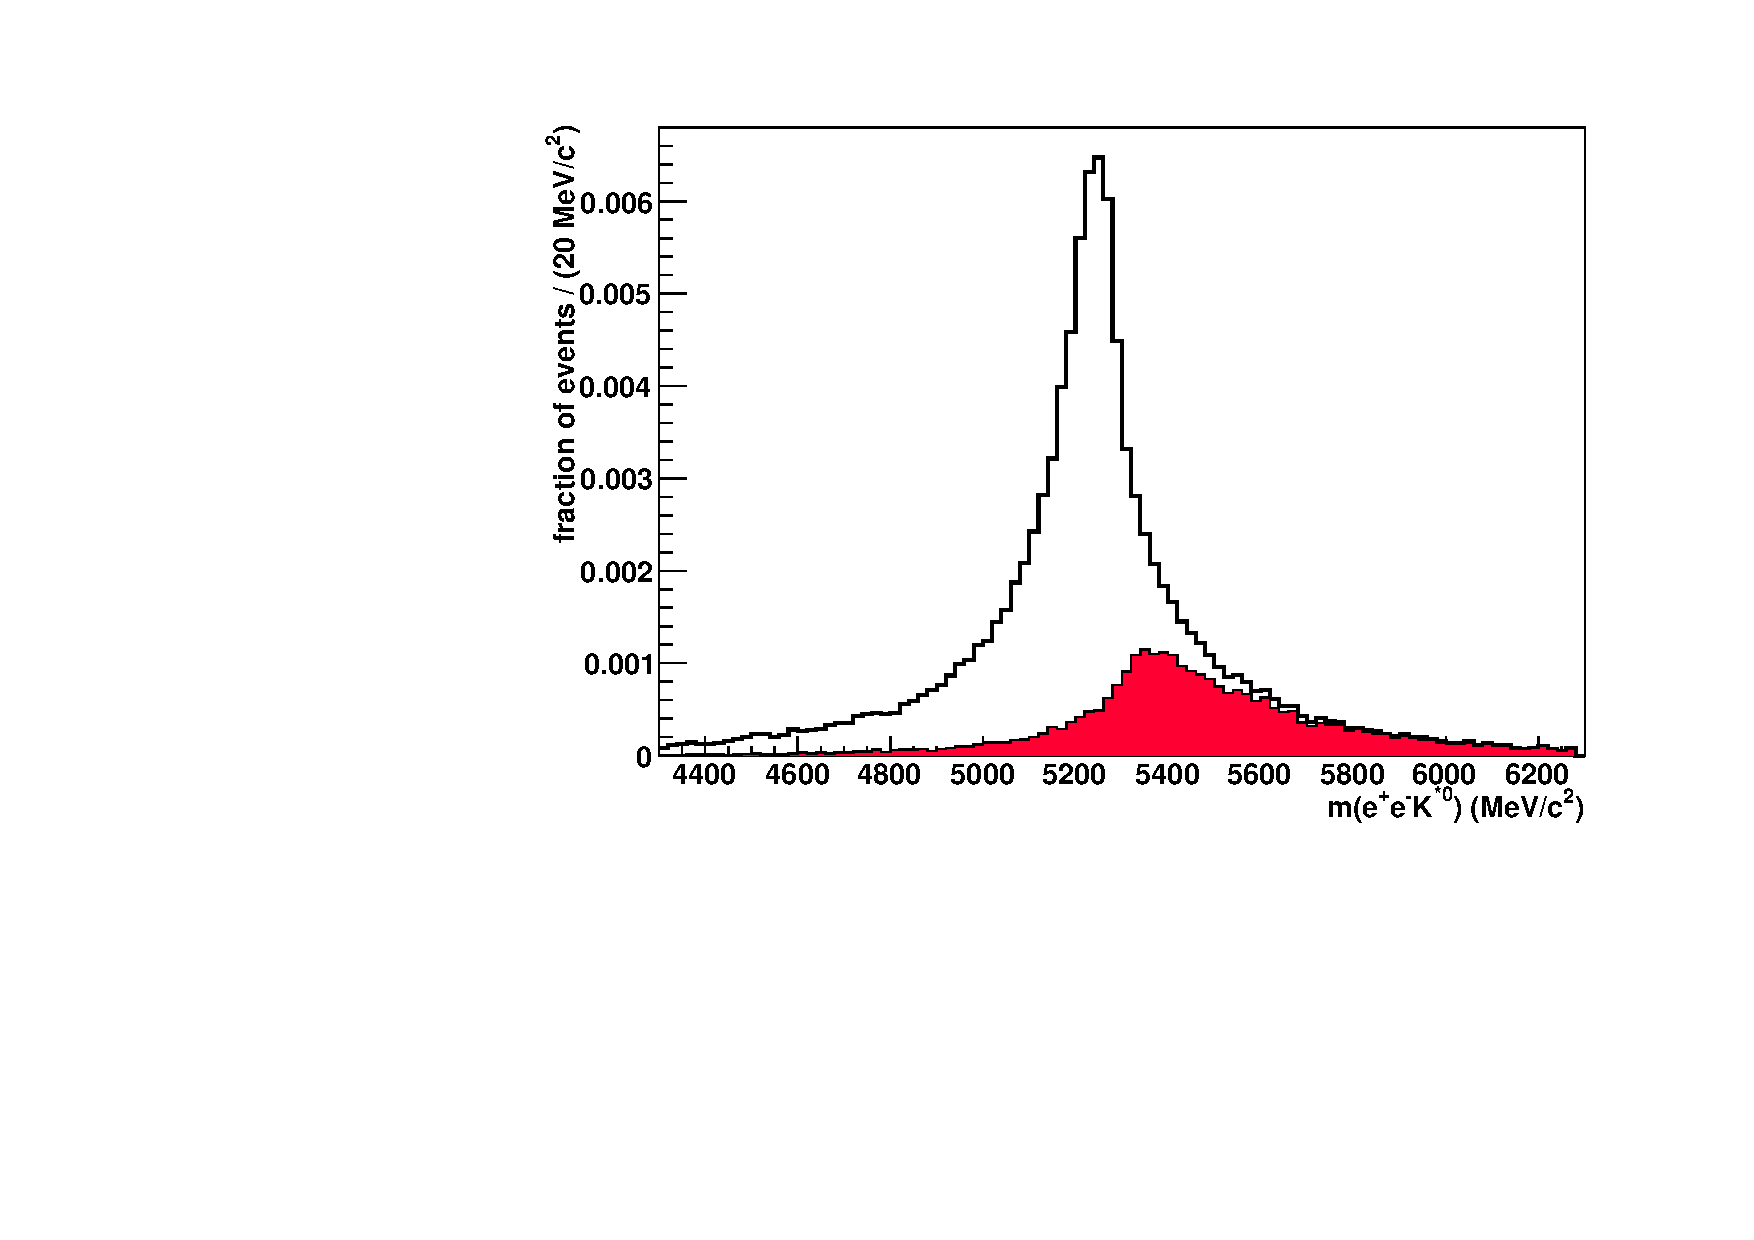
\includegraphics[width=0.49\textwidth]{MC_Bmass_dielectron_TM_nodccorrection_simplehisto.pdf}} 
  \subfigure{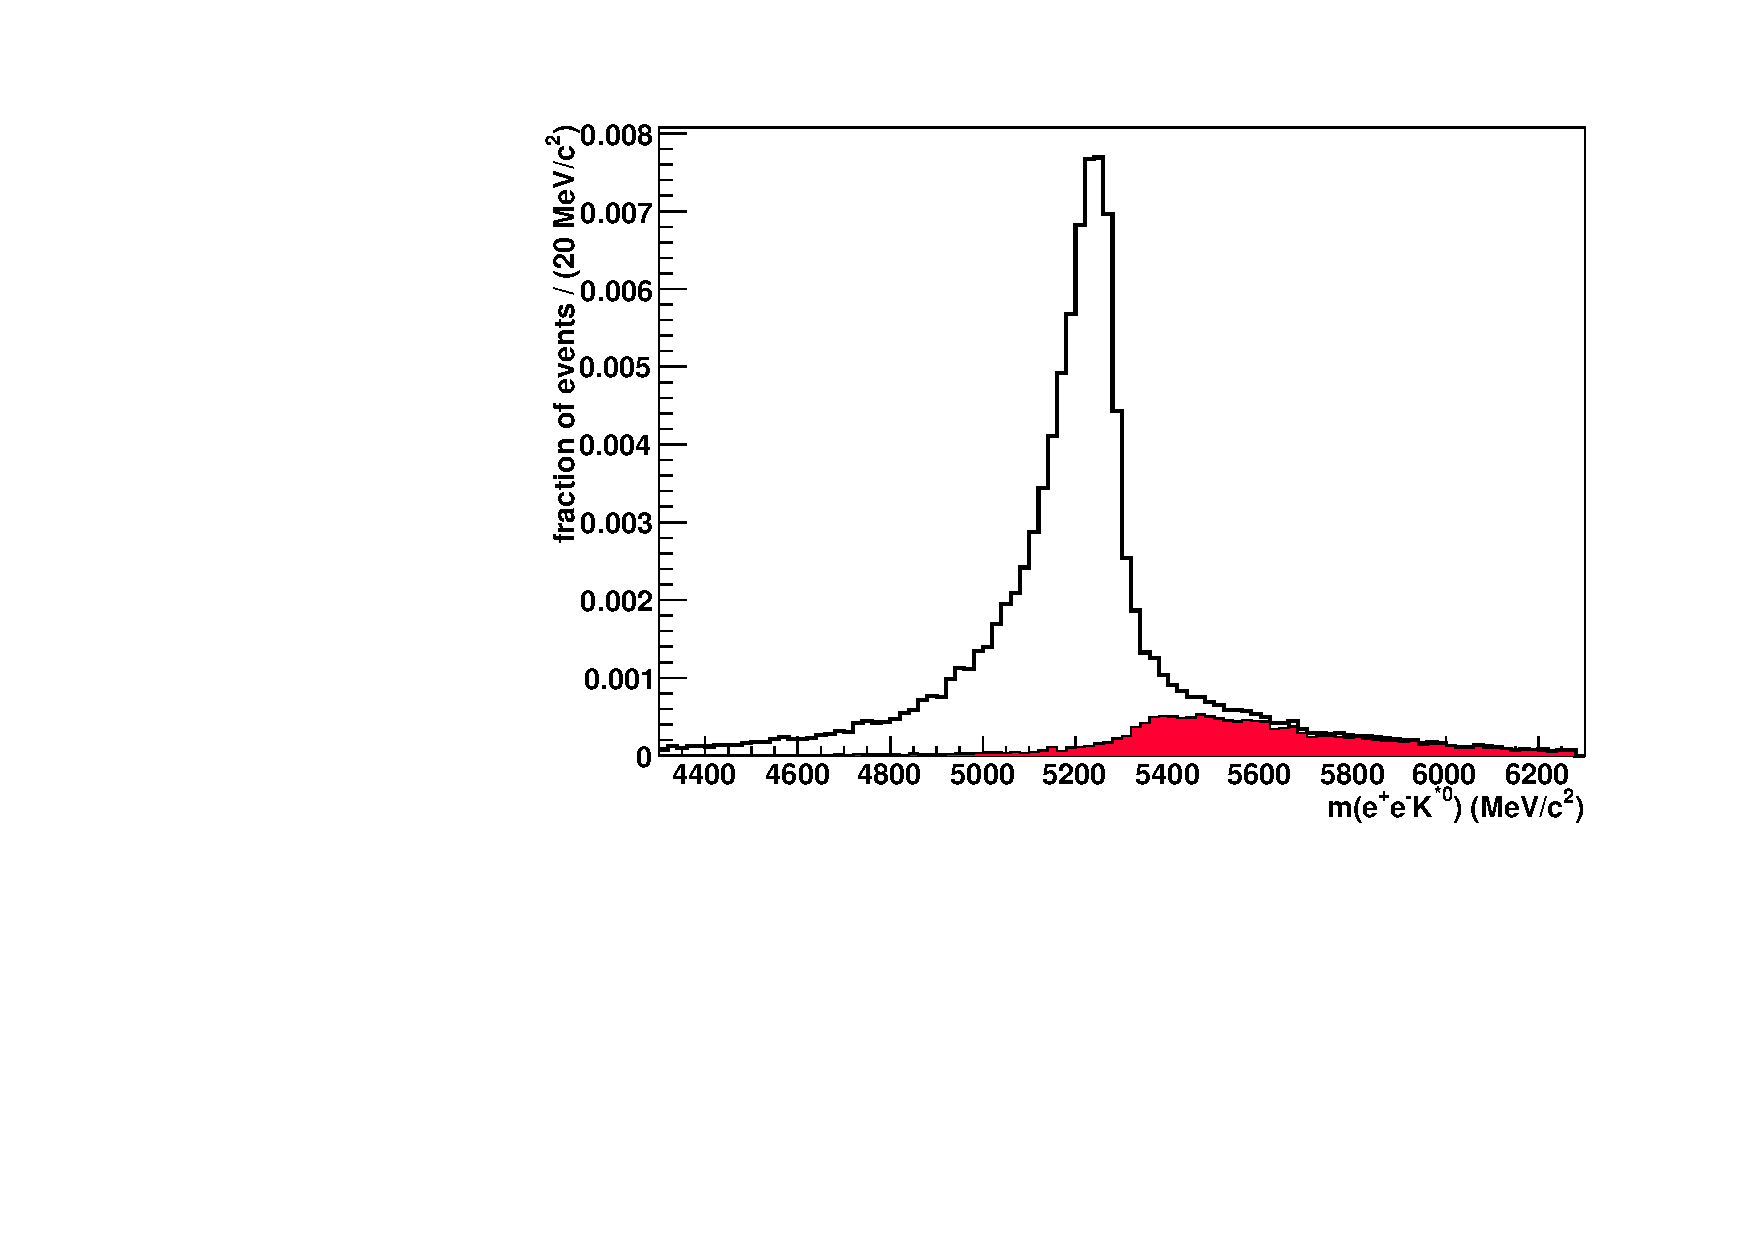
\includegraphics[width=0.49\textwidth]{MC_Bmass_dielectron_TM_nodccorrection_simplehisto_newBrem.pdf}}
  \vspace*{-1.0cm}
  \end{center}
  \caption{\textit{\Bd mass shape. The pink distribution are the events with double counting. The \Bd distribution is obtained by reconstructing \lhcb Monte Carlo with \davinci v29 (left) and \davinci v30 (right) respectively.}}
  \label{fig:oldBremAddernodcc}
\end{figure}
As can be seen from Figures \ref{fig:oldBremAddernodcc} and \ref{fig:Minveedouble counting} the amount of double counting is higher for the \davinci v29 bremsstrahlung recovery. The \lhcb Monte Carlo sample shows that double counting events account for 27 \% of all the signal events in \davinci 29 while it's only about 14\% of the signal events for \davinci v30. \\



\subsubsection{The double counting correction}
\label{sub:doublecountingcorrection}
In the course of the analysis four different methods to encounter the problem of double counting have been developed and tested:
\begin{compactenum}[a)]
\item The energy of the double counted photon candidate is assigned to the lepton with lower energy.
\item The energy of the double counted photon candidate is assigned to the lepton with higher energy.
\item The energy of the double counted photon candidate is assigned to a randomly chosen lepton. 
\item The energy of the double counted photon candidate is equally divided between the two leptons.
\end{compactenum}
After assigning the bremsstrahlung photon's energy, the four-momenta of the leptons is recalculated. From these new lepton four-momenta and the original four-momenta of the Kaon and the Pion the \Bd mass is recalculated.\\
The recalculated \Bd mass distributions for the four different methods applied to the \BdKstee \lhcb Monte Carlo sample made with the \davinci v29 are shown in Figure \ref{fig:double countingcorrection}. \\
While the first three methods yield extremely similar results, the fourth method does not reproduce the \Bd mass shape correctly. For further analysis the third method of encountering double counting is chosen. Assigning of the bremsstrahlung photon's energy to one randomly chosen electron does not undergo the risk of biasing any energy distribution and yields the most accurate \Bd mass reconstruction of the four tested algorithms.\\
\begin{figure}[ht]
\vspace*{-0.4cm}
  \begin{center}
    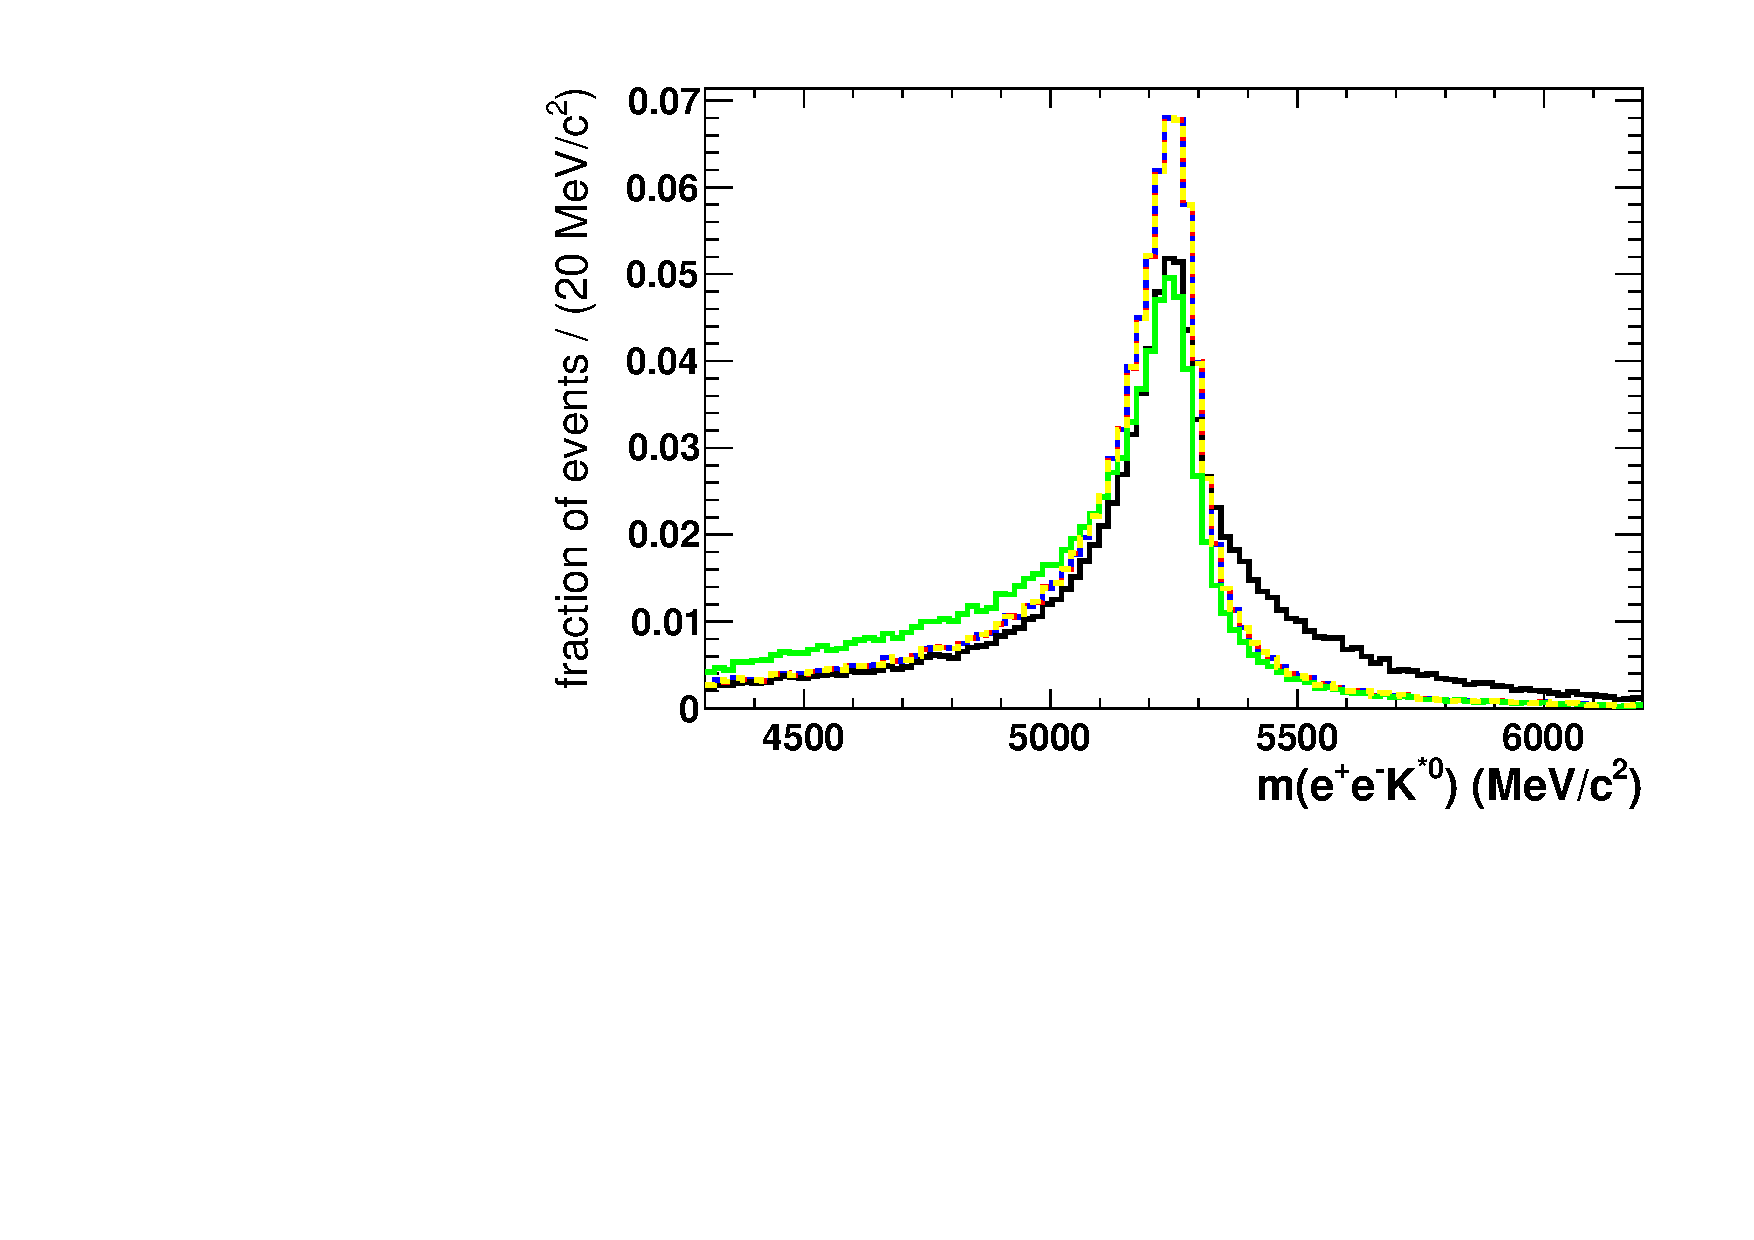
\includegraphics[scale=0.6]{minvB_nodccorrection.pdf}
  \vspace*{-1.0cm}
  \end{center}
  \caption{\textit{\Bd mass shapes for different algorithms of double counting correction. Black: no double counting correction; red: a); yellow: b); blue: c); green: d). }}
  \label{fig:double countingcorrection}
\end{figure}
\\

\subsection{Comparison of bremsstrahlung recovery algorithms}
The two bremsstrahlung recovery tools are applied to the \BdKstee \lhcb Monte Carlo, together with the double counting correction developed in the previous section. Additionally the selection developed for the 2011 dataset \cite{michellesthesis} is applied to the samples to estimate the effects on the final dataset.\\
To quantify the quality of the reconstruction tools a double Crystal-Ball distribution \cite{crystal} (for more details see Section \ref{sec:pdfs}) is fitted to the \Bd mass shape. The two Crystal-Ball distributions share the same $\mu_{\B}$, $\alpha$ and $n$. A weighted width $\sigma^w$ is calculated from the width $\sigma_1$ and $\sigma_2$ from the two Crystal-Ball distributions, where $f$ denotes the relative contribution from the first Crystal-Ball distribution.
\begin{equation}
\sigma^w = f \sigma_1 + (1- f) \sigma_2
\end{equation}

The two resulting distributions can be seen in Figure \ref{fig:comparebrems}. The resulting weighted resolutions are listed in Table \ref{tab:sigmaw}.

\begin{figure}[!h]
\vspace*{-0.cm}
  \begin{center}
  \subfigure{\label{fig:oldBremAdder}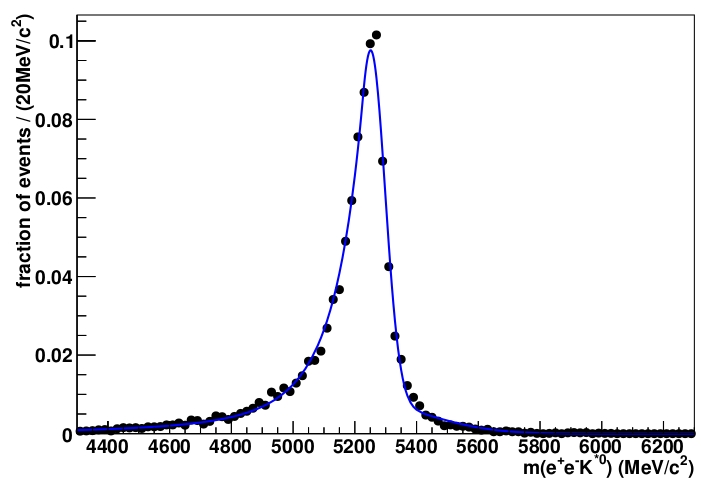
\includegraphics[width=0.49\textwidth]{oldBrem_crystalfit.jpg}}
  \subfigure{\label{fig:newBremAdder}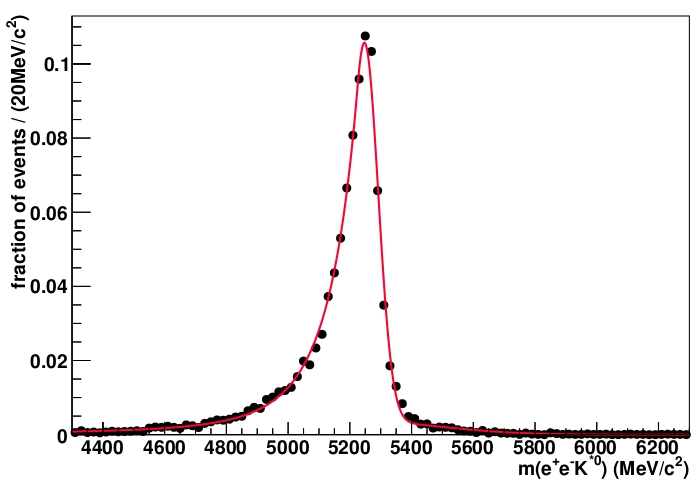
\includegraphics[width=0.48\textwidth]{newBrem_crystalfit.jpg}} 
  \vspace*{-1.0cm}
  \end{center}
  \caption{\textit{\Bd mass distribution obtained from \lhcb Monte Carlo with \davinci v29 (left) and \davinci v30 (right) and the double counting correction.}}
  \label{fig:comparebrems}
\end{figure}

\begin{table}[!h]
\begin{center}
\begin{tabular}{c|c|c|c|c}
& $\sigma_1$ & $\sigma_2$ & $f$ & $\sigma^w$ \\
\hline
\davinci v29 &  47 \mevcc & 199 \mevcc & 0.76 & 83 \mevcc \\
\hline
\davinci v30 & 45 \mevcc & 251 \mevcc & 0.86 & 74 \mevcc \\
\end{tabular}
\end{center}
\vspace*{-0.5cm}
\caption{\textit{Relevant results of the fit of a double Crystal-Ball distribution to the \BdKstee \lhcb Monte Carlo reconstructed with \davinci v29 and \davinci v30 and the double counting correction. $\sigma^w$ denotes the weighted width.}}
\label{tab:sigmaw}
\end{table}
By using the bremsstrahlung reconstruction in \davinci v30, the resolution of the \Bd mass can by increased about $13\ $\%. \\


\subsection{Effect of bremsstrahlung radiation and reconstruction on the \Bd mass shape}
Despite the implementation of the bremsstrahlung recovery tools, bremsstrahlung radiation affects the reconstructed \Bd mass shape. This can be seen in Figure \ref{fig:electronAndMuonBMass} where the reconstructed \Bd from \BdKstee is shown in direct comparison to the distribution of the \Bd mass from \BdKstmumu.\\
One effect is the large tail of the \Bd mass distribution from \BdKstee towards low \Bd masses. This tail originates from events whose bremsstrahlung photons could not be recuperated, resulting in a 
measured electron energy smaller than the initial electron energy $E^{measured}_{\epm} = (1 - E_{bs}) E^0_{\epm}$. \\
The second effect is the downgraded mass resolution which stems from the great uncertainty on the energy measurement of the calorimeter. In \lhcb the energy measurement of charged particle is performed by using combined information from the tracking system and the particle identification system. The tracking system determines the momentum of the charged particle $p_T^{track}$ with a relative accuracy of about $0.5 $\%. The particle identification system determines the identity of the particle which fixes the invariant mass of the particle track to the PDG value $m^{PDG}$. The particle's energy $E$ is then calculated from the combination of the measured momentum and the PDG \cite{pdg} \footnote{Particle Data Group.} mass.
\begin{equation}
E = \sqrt{p^2_{track} + m^2_{PDG}}
\end{equation}
The relative energy resolution is thus also of the order of $0.5 $\%.\\
For neutral particles however, the energy measurement has to be performed by the calorimeter. Since the relative energy resolution of the calorimeter is  
\begin{equation}
\frac{\sigma_E}{E} = \frac{10 \%}{\sqrt{E}} \oplus 1 \%
\end{equation}
the energy resolution of neutral particles is much worse than the energy resolution of charged particles.\\
Electrons, like muons, are charged particles and their tracks' transverse momenta $p_T^{track}(\epm)$ could be determined with an average relative accuracy of $0.5$\%. The energy of the bremsstrahlung photons however, has to be determined by the \ecal. The increase in uncertainty on the electron energy will propagate to the measured \Bd mass. \\
Figure \ref{fig:electronAndMuonBMass} shows the comparison between the \Bd mass shape of the \BdKstee and the \BdKstmumu.
\begin{figure}[ht]
  \begin{center}
  \subfigure{
  	\label{fig:eeKstar}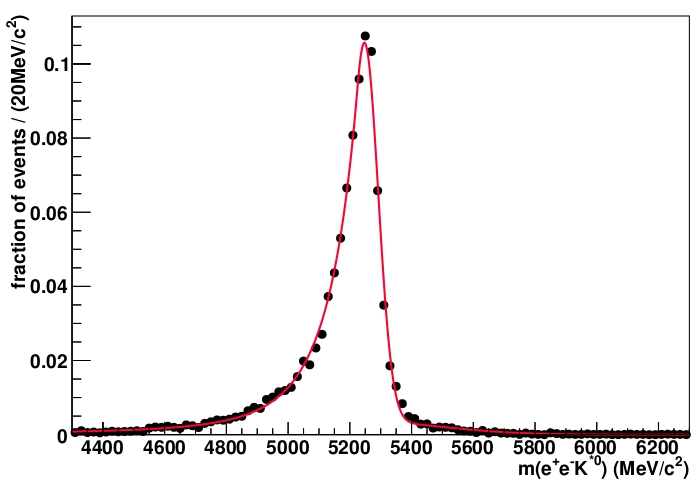
\includegraphics[width=0.49\textwidth]{newBrem_crystalfit.jpg}}
  \subfigure{\label{fig:mumuKstar}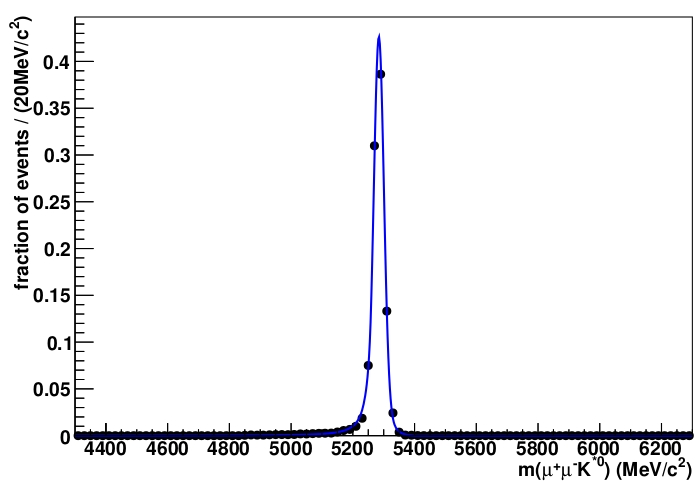
\includegraphics[width=0.49\textwidth]{MC_Bmass_mumuKstar_TM.jpg}} 
  \vspace*{-1.0cm}
  \end{center}
  \caption{\textit{Comparison of the \Bd mass distribution from \BdKstee (left) and \BdKstmumu (right) reconstructed from \lhcb Monte Carlo samples. The distribution from  \BdKstee is much wider and shows a tail at low \Bd masses, while the distribution for \BdKstmumu is just a very narrow peak.}}
  \label{fig:electronAndMuonBMass}
\end{figure}


\section{$M_{inv}(\epem)$ reconstruction}
\label{sec:DiElectronMaker}
The correct reconstruction of the invariant mass of the $e^+ e^-$ pair in the \BdKstee decay is crucial for the measurement of the various amplitudes contributing to the decay since they depend on the $M_{inv}(\epem)$ (see Chapter \ref{chapter1}).\\
In \davinci v31 a new tool designed to make opposite and same sign electron pairs was introduced. This tool -- the so-called \dielectronmaker  \ -- was specially developed to reconstruct low invariant mass $e^+ e^-$ pairs, such as electrons and positrons from converted photon or light resonances.\\
\\
While usually electron pairs are being made by combining two reconstructed electrons, the \dielectronmaker accesses the raw detector information for the electron and the positron candidates directly. Based on the hits associated to the two candidates' tracks the \dielectronmaker creates a \textit{DiElectron object} first and only then computes the properties of the individual electron and positron respectively. The \dielectronmaker chooses tracks with a $p_T$ greater than $100 \mevc$ as electron candidates. It composes the \textit{DiElectron object} from opposite sign electron pair tracks and then applies the bremsstrahlung recovery tool from \davinci v30. In the case of double counting within one \textit{DiElectron object} the four-momentum of the photon candidate is added to one randomly chosen electron, similarly to the double counting correction in Section \ref{sub:doublecountingcorrection}. Then the four-momenta of the \textit{DiElectron object} and the electron and the positron are calculated and a $p_T(e^+ e^-)$ cut greater than $500 \mevc$ is applied.
From this \textit{DiElectron object} the rest of the event reconstruction follows as usual.\\
\\
The \dielectronmaker was created to increase the efficiency of reconstruction for events with low invariant mass $e^+ e^-$ pairs and also yields a more precise reconstruction of the \Bd mass as can be seen on the Monte Carlo sample in Figure \ref{fig:diElectron}. Additionally the selection developed for the 2011 dataset \cite{michellesthesis} is applied to the sample to estimate the effects on the final dataset. The results of the fit of the double Crystal-Ball distribution to the sample are listed in Table \ref{tab:disigmaw}, showing that the use of this new tool decreases the $\sigma^w$ even further than the reconstruction by \davinci v30  yielding a reduction of $27 \ $\% with respect to the reconstruction implemented in \davinci v29.
\begin{figure}[ht]
  \begin{center}
  \subfigure{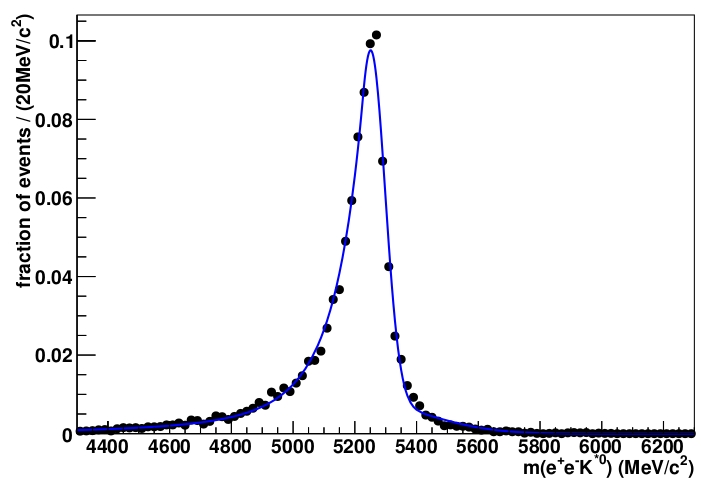
\includegraphics[width=0.49\textwidth]{oldBrem_crystalfit.jpg}}
  \subfigure{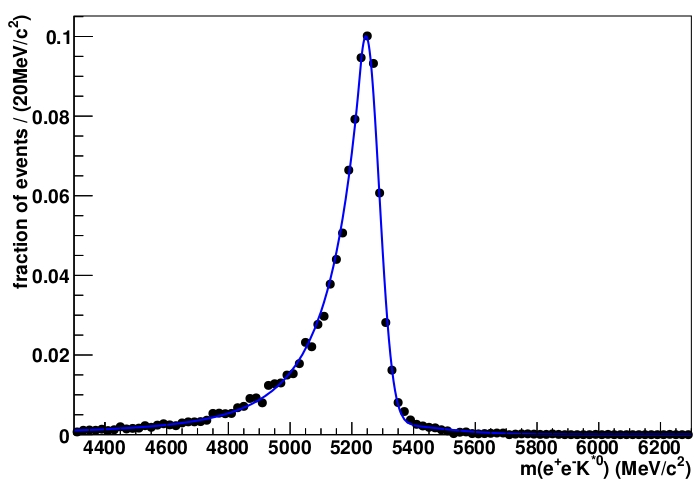
\includegraphics[width=0.49\textwidth]{diElectron_crystalfit.jpg}} 
  \end{center}
  \caption{\textit{\Bd mass distribution obtained from \lhcb Monte Carlo with \davinci v29 and double counting correction (left) and the \dielectronmaker of \davinci v31 (right).}}
  \label{fig:diElectron}
\end{figure}

\begin{table}[hc]
\begin{center}
\begin{tabular}{c|c|c|c|c}
& $\sigma_1$ & $\sigma_2$ & $f$ & $\sigma^w$ \\
\hline
\davinci v29 &  47 \mevcc & 199 \mevcc & 0.76 & 83 \mevcc \\
\hline
\davinci v31 & 54 \mevcc &  306 \mevcc & 0.91 &  77 \mevcc \\
\end{tabular}
\end{center}
\vspace*{-0.5cm}
\caption{\textit{Relevant results of the fit of a double Crystal-Ball distribution to the \BdKstee \lhcb Monte Carlo reconstructed with \davinci v29 and the double counting correction and \davinci v31. $\sigma^w$ denotes the weighted width.}}
\label{tab:disigmaw}
\end{table}

Figure \ref{fig:deltaee} shows the resolution of the dilepton invariant mass obtained from \BdKstee Monte Carlo for a dilepton invariant mass between 20\mevcc and 30\mevcc and 30\mevcc and 50\mevcc respectively. The resolutions are computed for the Monte Carlo sample that was processed with each  \davinci v29 and \davinci v31.\\
The plots show that the histograms from \davinci v31 are better centred and their Root Mean Square (RMS) is reduced by 20\% to 30\%. The first effect originates from the newer Bremsstrahlung recovery algorithm that is implemented in the \dielectronmaker. This recovery algorithm identifies more bremsstrahlung photons than the one in \davinci v29 and adds them to their emitting electron. The use of the \dielectronmaker reduces the RMS of the histograms with respect to those made by \davinci v29 because of the intermediate step of computing the \textit{DiElectron object}.
\begin{figure}[!h]
\vspace*{-0.cm}
  \begin{center}
    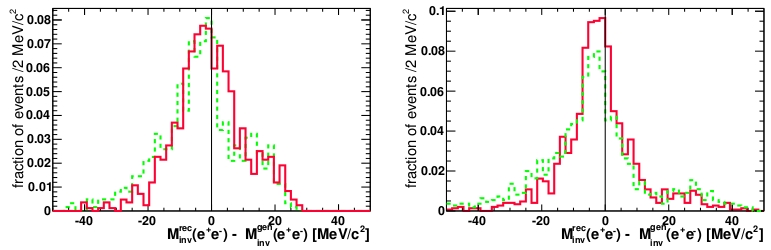
\includegraphics[scale=0.6]{deltaee.jpg}
  \vspace*{-0.5cm}
  \end{center}
  \caption{\textit{Resolution of the dilepton invariant mass obtained from the \BdKstee Monte Carlo. \textbf{Left:} The histograms for the region of 20\mevcc < $M^{gen}_{inv}(\epem)$ < 30\mevcc. \textbf{Right:} The histograms for the region of 30\mevcc < $M^{gen}_{inv}(\epem)$ < 50\mevcc. The green histogram represents the resolution of the sample processed with \davinci v29, the pink histogram represents the resolution of the sample processed with \davinci v31.}}
  \label{fig:deltaee}
\end{figure}
\\
\vspace*{1.cm}
\section{Comparison of reconstruction efficiencies}
To evaluate the performance of $M_{inv}(\epem)$ reconstruction the three reconstruction tools implemented in \davinci v29, \davinci 30 and \davinci v31 are applied to the \BdKstee \lhcb Monte Carlo respectively. After this, the double counting correction algorithm is executed on the first two samples and the selection developed for the 2011 dataset \cite{michellesthesis} \cite{paper} is applied to all three samples to estimate the effects on the final datasets.\\
Figure \ref{fig:eff_diElectron} shows the overall efficiency for reconstruction and selection of the three samples in dependency of the true -- that is generated -- invariant \epem mass $M^{gen}_{inv}(\epem)$. Note that there is a cut on the reconstructed invariant \epem mass $M^{reco}_{inv}(\epem)>30 \mevcc$\footnote{The selection developed for the 2011 dataset \cite{michellesthesis} \cite{paper} includes a tighter cut on the invariant dilepton mass than the selection developed in the course of this master's thesis}.\\
Figure \ref{fig:eff_diElectron} shows that the use of the \dielectronmaker yields the most accurate results and the highest reconstruction efficiency, especially in the region of highest interest between $30 \mevcc$ and $65 \mevcc$. The amount of reconstructed events with a generated invariant mass below $30 \mevcc$ is zero up to almost $15 \mevcc$ and then smoothly increases due to multiple scattering.\\
Above $65 \mevcc$ the efficiencies for all three reconstruction algorithms converge to the same value and remain independent of the generated invariant \epem mass.\newpage
\begin{figure}[!h]
  \begin{center}
    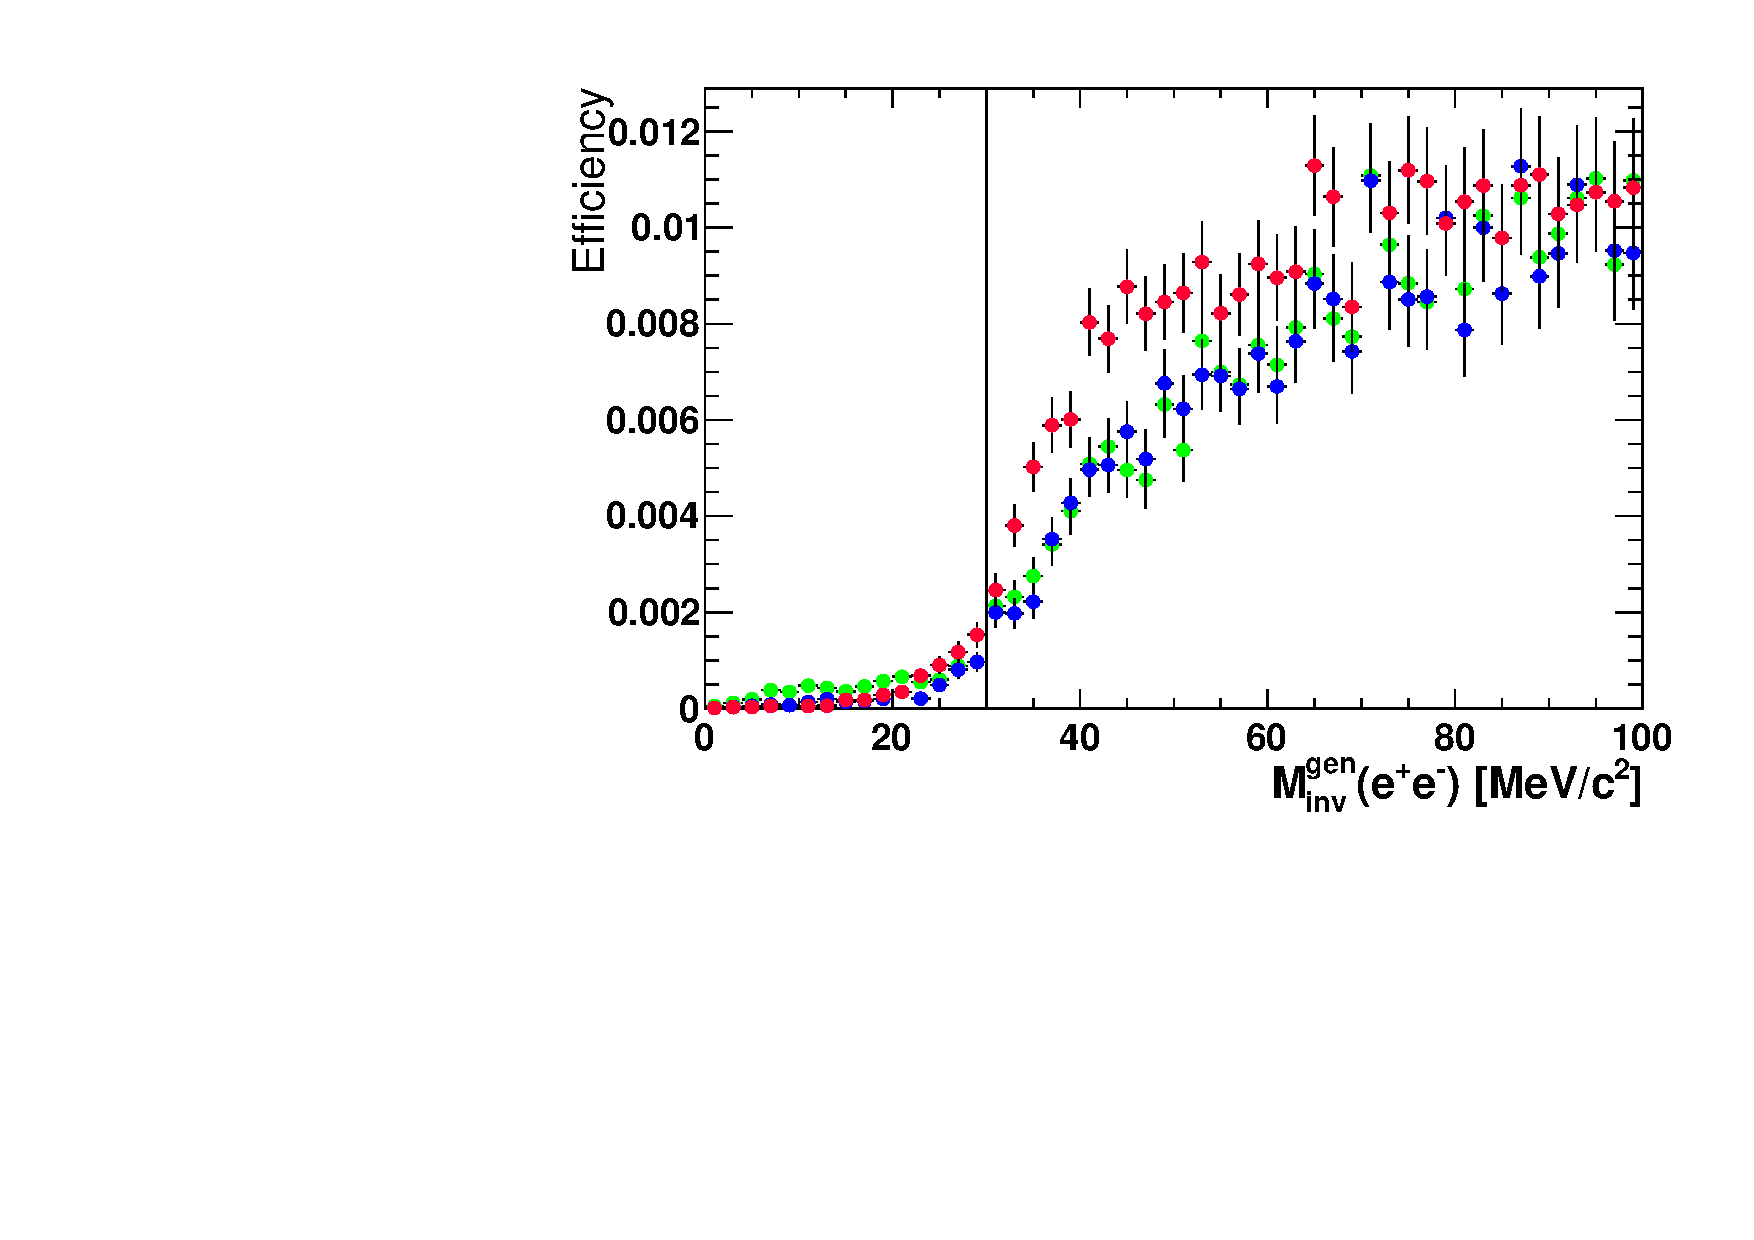
\includegraphics[scale=0.6]{eff_diElectron.pdf}
  \vspace*{-0.5cm}
  \end{center}
  \caption{\textit{Absolute event reconstruction and selection efficiency depending on the generated $M^{gen}_{inv}(\epem)$. Obtained from \BdKstee Monte Carlo by comparing the $M^{gen}_{inv}(\epem)$ at generator level with the $M^{rec}_{inv}(\epem)$ distribution after reconstruction and selection. Green: \davinci v29, blue: \davinci v30, pink: \davinci v30 with \dielectronmaker .}}
  \label{fig:eff_diElectron}
\end{figure}
\vspace*{10cm}


%%%%%%%%%%%%%%%%%%%%%%%%%%%%%%%%%%%%%%%%%%%%%%%%%%%%%%%%%%%%%%%%%%%%%%%%%%%%%%%%%%%%%%%%%%%%%%%%%%%%%%%%%%%%
%Events with double counting were identified by comparing the energy of the Bremsstrahlung photon. If this energy was non zero and the same for the photon coming %from the electron and from the positron within $5 \mev$, the event was considers to be a double counting event.

%To compare the performance of the two n-tuples of \lhcb \BdKstee Monte Carlo are created with the different bremsstrahlung recovery algorithms respectively. Then %the double counting correction is applied to both n-tuples.\\

%\subsection{DaVinci v29r1p1 BremAdder}
%\label{sub:oldBrem}
%As a first step a NTuple was created using DaVinci v29r1p1 and its standard Bremsstrahlung recovery tool. This BremAdder matches photons to the electrons by lineraly extrapolating the
%electron track from its last state before the TT to the calorimeter. If the $\chi_{brem}^2$ of the extrapolated track and the photon position in the calorimeter is less than 300, this photon is
%considerd a bremsphoton and its energy is added to the electron.\\
%Complementing this BremAdder algorithm by the \textit{double counting- correction} yields the $B^0$ mass shape in \ref{fig:oldBremAdder}. The weighted sigma of this shape is $\sigma_{w} = $.\\
%\begin{figure}[ht]
%  \begin{center}
%    \includegraphics[scale=0.6]{figs/Bmass_oldBremdcc.pdf}
%  \vspace*{-1.0cm}
%  \end{center}
%  \caption{$B^0$ mass shape for the DaVinci v29r1p1 bremsstrahlung recovery tool and double- counting correction}
%  \label{fig:oldBremAdder}
%\end{figure}
%
%\subsection{DaVinci v31r0 BremAdder}
%\label{sub:newBremAdder}
%For the second procedure a NTuple was created using DaVinci v31r0 and its standard Bremsstrahlung recovery tool. This new BremAdder is an enhanced version of the BremAdder in \ref{sub:oldBrem}. It
%uses the StdAllLoosePhotons as bremsphoton candidates by default. A photon is matched as a bremsphoton if:
%\begin{itemize}
% \item its X- position in the calorimeter is between the extrapolated X- position of the electrons first state and its extrapolated X- position from the TT within $n_x \cdot \sigma_x$ (default:
%$n_x = 2$, $\sigma_x =$ quadratic sum of photon cluster spread and track extrapolation uncertainty)
%\item its Y- position in the calorimeter matches the extrapolated Y- position from the TT within $n_y \cdot \sigma_y$ (default: $n_y = 2$, $\sigma_y =$ quadratic sum of photon
%cluster spread and track extrapolation uncertainty).
%\end{itemize}
%Complementing this BremAdder algorithm by the \textit{double counting- correction} yields the $B^0$ mass shape in \ref{fig:newBremAdder}. The weighted sigma of this shape is $\sigma_{w} = $.\\
%\begin{figure}[ht]
%  \begin{center}
%    \includegraphics[scale=0.6]{figs/Bmass_newBremdcc.pdf}
%  \vspace*{-1.0cm}
%  \end{center}
%  \caption{$B^0$ mass shape for the DaVinci v31r0 bremsstrahlung recovery tool and double- counting correction}
%  \label{fig:newBremAdder}
%\end{figure}
%
%
%\subsection{DaVinci v32 DiElectronMaker}
%\label{sub:DiElectronMaker}
%For the DaVinci v31r0 a new tool to make $e^+ e^-$ pairs has been developed (also configurable to find same sign pairs). This Tool - called \textit{DiElectronMaker} - takes the electron ProtoParticles
%and creates low invariant mass $e^+ e^-$ pairs. The DiElectronMaker uses a method of the new BremAdder (from the DaVinci v31r0) which makes it possible to avoid the double counting. In the
%case of one bremsphoton candidate matching both electrons this method adds the bremsphoton to one randomly chosen electron - 
%The DiElectronMaker then selects $e^+ e^-$ pairs that pass
%
%
%
%
%\begin{figure}[ht]
%  \begin{center}
%    \includegraphics[scale=0.6]{figs/Bmass_diElectron.pdf}
%  \vspace*{-1.0cm}
%  \end{center}
%  \caption{$B^0$ mass shape for the DaVinci v31r0 DiElectronMaker}
%  \label{fig:diElectronMaker}
%\end{figure}
%\section{Effect of bremsstrahlung radiation on the \Bd mass shape}
%The emittance of bremsstrahlung photons has two different effects on the reconstructed \Bd mass shape.\\
%The first effect can be seen on the Monte Carlo sample in Figure \ref{fig:noBremReco}. If the bremsstrahlung photons are not recuperated the measured electron energy will be smaller than the initial electron energy $E^{measured}_{\epm} = (1 - E_{bs}) E^0_{\epm}$ and this offset will propagate to the reconstructed \Bd mass. Figure \ref{fig:noBremReco} shows the \Bd mass distribution obtained without any bremsstrahlung reconstruction. The distribution has an asymmetric, non Gaussian shape with a very large radiative tail in the low \Bd mass region. Since this tail diminishes the resolution on the \Bd mass and even exceeds the reconstructed mass region, it is crucial to recuperate the emitted bremsstrahlung photons and associate them to their electrons.\\
%This bremsstrahlung recovery causes the second effect on the measured \Bd mass distribution.
%In \lhcb the energy measurement of charged particle is performed by using combined information from the tracking system and the particle identification system. The tracking system determines the momentum of the charged particle $p_T^{track}(c.p.)$ with an accuracy of about $0.5 /$\%. The particle identification system determines the identity of the particle which fixes the invariant mass of the particle track to the PDG value $m_{PDG}(c.p.)$. The particle's energy is then calculated from the combination of the measured momentum and the PDG mass $E(c.p.) = \sqrt{p^2_{track}(c.p.) + m_{PDG}(c.p.)}$. This allows for an energy resolution of the order of the momentum resolution for charged particles.\\
%For neutral particles however, the energy measurement has to be performed by the calorimeter. Since the energy resolution of the calorimeter is much worse than the momentum resolution obtained by the tracking system, the energy resolution of neutral particles is much worse than the energy resolution of charged particles.\\
%Electrons, like muons, are charged particles and their tracks' transverse momenta $p_T^{track}(\epm)$ could be determined with an accuracy up to $0.35$\%. The energy of the bremsstrahlung photons however, has to be determined by the \ecal. The increase in uncertainty on the electron energy will be propagate to the measured \Bd mass. In particular, the \Bd mass distribution reconstructed from \BdKstee will show a greater width than the \Bd mass distribution reconstructed from \BdKstmumu for example.
%Figure \ref{fig:electronAndMuonBMass} shows the comparison between the \Bd mass shape of the \BdKstee and the \BdKstmumu.
%\begin{figure}[ht]
%  \begin{center}
%  \subfigure{
%  	\label{fig:eeKstar}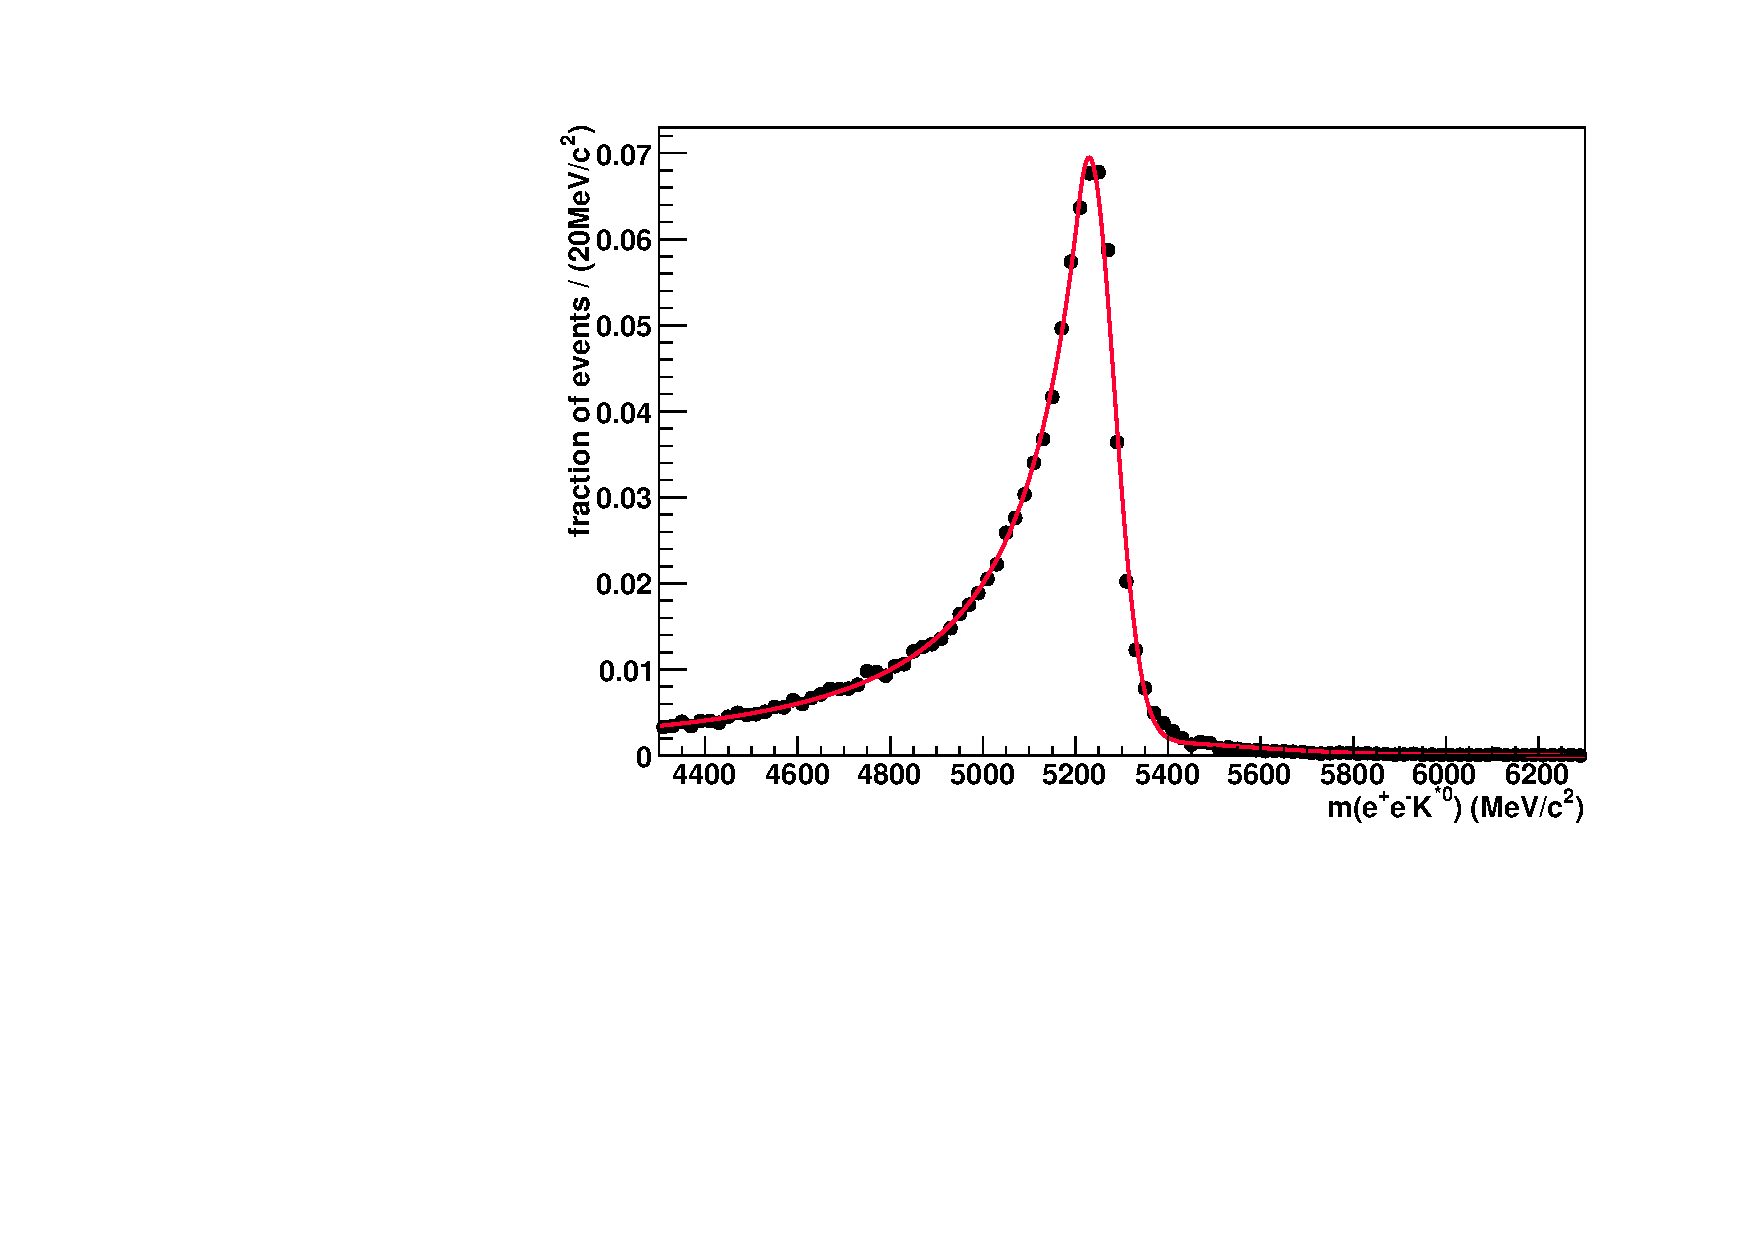
\includegraphics[width=0.49\textwidth]{MC_Bmass_dielectron_TM.pdf}}
%  \subfigure{\label{fig:mumuKstar}\includegraphics[width=0.49\textwidth]{MC_Bmass_mumuKstar_TM.pdf}} 
%  \vspace*{-1.0cm}
%  \end{center}
%  \caption{\textit{Comparison of the \Bd mass distribution from \BdKstee (left) and \BdKstmumu (right) reconstructed from \lhcb Monte Carlo samples.}}
%  \label{fig:electronAndMuonBMass}
%\end{figure}

%\chapter{Systematic uncertainties}
\label{c:sys}
\section{Sources of systematic uncertainties}
\\
\subsection{Non-flat flat and continuum bkg}
\label{s:flat}
In order to evaluate the effect of the flat and continuum bkg possibly not being flat the distribution of flat bkg in \KsPiPi  is taken from generic MC. \\
Since it is known that the continuum MC does not model the distribution well, another approach is chosen for the \KlPiPi bkg. From data the sideband defined by $-0.1 < m_{miss}^2 < 0.1$ and $1.83 < m_{BC} < 1.85$ is selected as it contains both flat bkg and continuum bkg but no peaking bkg. The distribution of events in this sideband is chosen to represent the flat and continuum bkg.\\


\subsection{Peaking bkg distribution}
\label{s:peak}
There are different components to the systematic uncertainty from the peaking bkg distribution:
\subsubsection{Limited data and MC sample}
\label{s:peaka}
 Uncertainty from the limited data and MC used to execute the procedure described in Section \ref{sec:peak} and Section \ref{sec:klpeak}.\\
	This uncertainty is calculated directly and listed with the default results in Table \ref{tab:MMKs} and Table \ref{tab:MMKl} for \4Pi vs \KsPiPi and \4Pi vs \KlPiPi respectively.\\

\subsubsection{Cleanness of data sample}
\label{s:peakb}
Uncertainty from the cleanness of the data samples used to determine the distribution of peaking bkg events where the reconstructed \4Pi comes from a \KsPiPi decay(see Sections \ref{sec:clean} and \ref{sec:klclean}). The effect of this systematic is estimated by assuming that the data sample consists of 96\% and 92\% peaking bkg events while the rest of the events is are distributed according to the generic MC.\\

\subsubsection{Unknown BR($\Dz \rightarrow \KlPiPi$)}
\label{s:peakc}
Uncertainty in the \4Pi vs \KlPiPi case on the total number of \KlPiPi vs \KlPiPi bkg events in the data sample.\\
	This uncertainty occurs due to the extrapolation of peaking bkg events from generic MC. Since the branching fraction of \D to \KlPiPi is not known, this number cannot be exact. To estimate this uncertainty the number of peaking bkg events is varied by $\pm$ 20\%.\\



\subsection{Multiple candidate selection}
\label{s:mcs}
A different multiple candidate selection is tested. Instead of selecting the best candidate based on $m_bc$ a candidate is chosen at random.\\
%the candidate with the smallest average $\Delta E$ is chosen. \\

\subsection{Dalitz plot acceptance}
\label{s:dpa}
The Dalitz plot acceptance is estimated in bins of pion track momentum $p$ and angle $\theta$ as described in Chris report.\\
\begin{table}[h!]
\begin{center}
\begin{tabular}{c | c c c c}
&  & $ \theta$ bin \\
\hline
\textbf{p} bin & 1 & 2 & 3 & 4\\ 
\hline
1 & 0.912 $\pm$ 0.006 & 1.010 $\pm$ 0.006 & 0.997 $\pm$ 0.006 & 0.976 $\pm$ 0.006 \\ 
2 & 0.972 $\pm$ 0.006 & 1.060 $\pm$ 0.006 & 1.060 $\pm$ 0.006 & 1.040 $\pm$ 0.006 \\ 
3 & 0.962 $\pm$ 0.006 & 1.050 $\pm$ 0.006 & 1.040 $\pm$ 0.006 & 1.030 $\pm$ 0.006 \\ 
4 & 0.876 $\pm$ 0.008 & 0.984 $\pm$ 0.009 & 0.979 $\pm$ 0.009 & 0.938 $\pm$ 0.008 \\ 
\end{tabular}
\end{center}
\caption{\textit{Normalized Dalitz plot efficiency for \4Pi vs \KsPiPi.}}
\end{table}


\begin{table}[h!]
\begin{center}
\begin{tabular}{c c c c c}&  & $ \theta$ bin \\
\hline
\textbf{p} bin & 1 & 2 & 3 & 4\\ 
\hline
1 & 0.912 $\pm$ 0.005 & 1 $\pm$ 0.006 & 1.01 $\pm$ 0.005 & 0.976 $\pm$ 0.004 \\ 
2 & 0.973 $\pm$ 0.004 & 1.06 $\pm$ 0.006 & 1.06 $\pm$ 0.005 & 1.04 $\pm$ 0.004 \\ 
3 & 0.966 $\pm$ 0.005 & 1.05 $\pm$ 0.006 & 1.05 $\pm$ 0.005 & 1.03 $\pm$ 0.004 \\ 
4 & 0.853 $\pm$ 0.006 & 0.967 $\pm$ 0.007 & 0.968 $\pm$ 0.007 & 0.924 $\pm$ 0.006 \\ 
\end{tabular}
\end{center}
\caption{\textit{Normalized Dalitz plot efficiency for \4Pi vs \KlPiPi.}}
\end{table}
\clearpage
\section{Effects on the number of signal events in \4Pi vs \KsPiPi}

\begin{table}[h!]
\begin{center}
\begin{tabular}{c |c |c |c |c | c}
bin i & default & \ref{s:flat} & \ref{s:peakb} & \ref{s:mcs} & \ref{s:dpa} \\
\hline
1 & 30.78 $\pm$ 6.97 $\oplus$ 0.24 $\oplus$ 0.65 & 31.13 & 30.69 & 29.68 & 28.60 \\ 
\hline
2 & 19.83 $\pm$ 5.25 $\oplus$ 0.27 $\oplus$ 0.45 & 18.64 & 19.79 & 19.44 & 20.29 \\ 
\hline
3 & 16.38 $\pm$ 4.47 $\oplus$ 0.27 $\oplus$ 0.50 & 16.73 & 16.34 & 15.8  & 15.03 \\ 
\hline
4 & 10.15 $\pm$ 3.38 $\oplus$ 0.18 $\oplus$ 0.30 & 10.63 & 10.16 & 12.30 & 7.96 \\ 
\hline
5 & 55.14 $\pm$ 8.04 $\oplus$ 0.68 $\oplus$ 0.56 & 54.22 & 55.11 & 50.81 & 54.91 \\ 
\hline
6 & 21.08 $\pm$ 5.08 $\oplus$ 0.33 $\oplus$ 0.38 & 20.29 & 21.11 & 21.98 & 21.47 \\ 
\hline
7 & 27.67 $\pm$ 5.94 $\oplus$ 0.43 $\oplus$ 0.57 & 28.50 & 27.86 & 27.20 & 29.17 \\ 
\hline
8 & 36.88 $\pm$ 6.78 $\oplus$ 0.45 $\oplus$ 0.62 & 37.73 & 36.82 & 32.06 & 35.99 \\ 
\end{tabular}
\end{center}
\caption{\textit{\4Pi vs \KsPiPi efficiency corrected and bkg subtracted signal events for different systematic effects. The first error on the default values is statistical, the second one from uncertainty on the signal efficiency and the third one is the uncertainty from the limited data and MC sample used to determine the distribution of peaking bkg events(Section \ref{s:peaka}). The systematic effects are from left to right: non-flat bkg, peaking bkg (cleanness of data sample 96\%), multiple candidate selection, Dalitz plot acceptance. }}
\end{table}

\section{Effects on the number of signal events in \4Pi vs \KlPiPi}
\begin{table}[h!]
\begin{center}
\begin{tabular}{c |c |c |c |c | c | c| c}
bin i & default & \ref{s:flat} & \ref{s:peakb} & \ref{s:peakc} & \ref{s:peakc} & \ref{s:mcs} & \ref{s:dpa} \\
\hline
1 & 134.11 $\pm$ 13.89 $\oplus$ 0.75 $\oplus$ 1.03 & 130.86 & 134.13 & 136.48 & 131.73 & 132.90 & 132.8 \\ 
\hline
2 & 59.23 $\pm$ 8.89 $\oplus$ 0.58 $\oplus$ 0.66 & 60.70 & 59.24 & 59.98 & 58.46 & 60.44 & 62.05 \\ 
\hline
3 & 55.39 $\pm$ 8.63 $\oplus$ 0.75 $\oplus$ 0.64 & 57.59 & 55.36 & 55.99 & 54.78 & 55.04 & 54.40 \\ 
\hline
4 & 20.34 $\pm$ 5.74 $\oplus$ 0.28 $\oplus$ 0.46 & 22.52 & 20.37 & 20.65 & 20.02 & 18.21 & 19.45 \\ 
\hline
5 & 46.01 $\pm$ 8.64 $\oplus$ 0.42 $\oplus$ 0.65 & 48.41 & 46.04 & 46.76 & 45.25 & 45.15 & 46.96 \\ 
\hline
6 & 24.58 $\pm$ 6.22 $\oplus$ 0.29 $\oplus$ 0.42 & 24.67 & 24.61 & 24.92 & 24.23 & 24.43 & 24.59 \\ 
\hline
7 & 61.16 $\pm$ 8.97 $\oplus$ 0.70 $\oplus$ 0.71 & 58.94 & 61.11 & 61.97 & 60.34 & 62.27 & 61.44 \\ 
\hline
8 & 84.13 $\pm$ 10.70 $\oplus$ 0.76 $\oplus$ 0.81 & 81.23 & 84.10 & 85.26 & 82.99 & 83.66 & 85.41 \\ 
\end{tabular}
\end{center}
\caption{\textit{\4Pi vs \KsPiPi efficiency corrected and bkg subtracted signal events for different systematic effects. The first error on the default values is statistical, the second one from uncertainty on the signal efficiency and the third one is the uncertainty from the limited data and MC sample used to determine the distribution of peaking bkg events(Section \ref{s:peaka}). The systematic effects are from left to right: non-flat bkg, peaking bkg (cleanness of data sample 92\%), peaking bkg (BR($\Dz \rightarrow \KlPiPi$) 20\% smaller than in genMC), peaking bkg (BR($\Dz \rightarrow \KlPiPi$) 20\% greater than in genMC), multiple candidate selection, Dalitz plot acceptance. }}
\end{table}
%\chapter{The \BdKstee signal yields}
\chaptermark{Chapter6}
\label{Chapter5}
After the set of preselection, optimised and veto cuts have been applied to the \\3 \invfb of data collected by \lhcb in 2011 and 2012 the signal yields are extracted. Therefore a probability density function (\PDF) is fitted to the resulting data sample. The entire fitting procedure is performed for each trigger category independently. The function of the \PDF is the same for all trigger categories but the parameters can vary.\\
The \PDF for the \BdKstee \lhcb data consists of different components that will be explained in the next section. Since the statistics of the final \BdKstee candidates is low the parameters of the \PDF for the \BdKstee data will be constrained using the \BdKstee Monte Carlo and also the \BdToJPsieeKst Monte Carlo and data. The \BdKstee Monte Carlo is used to constrain the shape of the signal while the more numerous \BdToJPsieeKst events are used to account for differences between Monte Carlo and \lhcb data and also to extract information about the background. The procedure of constraining the parameters is explained in Section \ref{sec:fitstrat} followed by the fit of the \PDF to the \BdKstee data and the extraction of signal and background yields.\\
At the end of this chapter the results obtained by the selection developed in this master's thesis are compared to the results that would have been obtained by adopting the selection developed on the 2011 \lhcb data.\\

\section{The components of the Probability Density Function}
\label{sec:pdfs}
The final \PDF for both the \BdKstee and the \BdToJPsieeKst candidates consists of a \PDF for the signal and a \PDF for the background. The background \PDF itself is composed of different components, namely the \textit{combinatorial background} and the \textit{partially reconstructed background}. These \PDF will be explored in the following.\\

\subsection{The signal \PDF}
Due to the energy loss of the electrons through bremsstrahlung radiation a double Crystal-Ball distribution (CB)\cite{crystal} was chosen for the the signal \PDF. \\
A CB distribution consists of a Gaussian core and a power law tail used to model the effect of energy loss during the reconstruction process. The CB function is described by:\\
\begin{equation}
CB(x;\alpha,n,\mu,\sigma) =  \begin{cases} \exp(- \frac{(x - \mu)^2}{2 \sigma^2}), & \mbox{for }\frac{x - \mu}{\sigma} > -\alpha \\ \frac{\left(\frac{n}{|\alpha|}\right)^n e^{-\frac{\alpha^2}{2}} }{\left(\frac{n}{|\alpha|} - |\alpha| -x\right)^n}, & \mbox{for }\frac{x - \mu}{\sigma} \leqslant -\alpha \end{cases} 
\end{equation}
where $\mu$ is the mean of the distribution, $\sigma$ the width, $\alpha$ the transition point from a Gaussian distribution to a power law tail distribution and $n$ the exponent of the power law tail.\\
The signal \PDF is modelled by the sum of two CBs to account for different resolution effects of the \lhcb detector. Therefore the CB distributions share the same mean $\mu$, $\alpha$ and $n$ but do have different widths $\sigma_1$ and $\sigma_2$. Furthermore there is a fraction $f$ between these two CBs.
\begin{equation}
\PDF^{sig} \ = \ f\ CB(x;\alpha,n,\mu,\sigma_1) + (1-f)\ CB(x;\alpha,n,\mu,\sigma_2)
\label{eq:dcb}
\end{equation}
\\
\subsection{The background \PDF}
The background in the \BdKstee decay consists of a \textit{combinatorial background} and a \textit{partially reconstructed background}. The combinatorial background originates from the matching of random tracks in the event that do not come from the same \B meson. The partially reconstructed background on the other hand comes from decays of \B mesons that are not fully reconstructed, that is where one or more tracks are not recuperated.\\

\subsubsection{The \PDF of combinatorial background}
The combinatorial background is fitted with an exponential function for each data sample individually and no constrains are applied.\\
\begin{equation}
\PDF^{comb. bkg} \ = e^{bx}
\end{equation}
\\
\subsubsection{The \PDF of partially reconstructed background}
The partially reconstructed background for the \BdKstee data comes from decays where the electrons originate from the \B meson while the \Kstarz meson is the decay product of an intermediate resonance. This means that the \B meson decay is of the form $\B \rightarrow \epem Y(\rightarrow \Kstarz X)$ where the $X$ is not reconstructed. This background also occurs for the \BdToJPsieeKst.\\
Another kind of partially reconstructed background that only exists for the\\ \BdToJPsieeKst but not for the \BdKstee is of the form\\ $B \rightarrow A (\rightarrow \jpsi B) \Kstarz$ where the $B$ is not reconstructed. This background does not occur for the \BdKstee since the electrons from \BdKstee can not come from any intermediate resonance due to the low dielectron invariant mass\footnote{The only resonance lying in the \epem invariant mass window is the $\rho$ giving $B \rightarrow \rho(\rightarrow \epem) \Kstarz$ which would be a peaking background instead of a partially reconstructed background. However, the contribution of the $\rho$ resonance has been found to be highly negligible.}. Since a full fit on the \BdToJPsieeKst data will be performed this background has to be modelled. \\
\\
The shapes of these two types of partially reconstructed background are determined separately using 1.3 million $\Bd \rightarrow \jpsi \Kstarz X$ and $\Bu / \Bub \rightarrow \jpsi \Kstarz X$ inclusive Monte Carlo events. The \PDF of each type of partially reconstructed background is then represented by a non-parametric function called ``\roopdf ''\cite{rookeys} implemented in \root \footnote{The \roopdf is a class of the \roofit package. It is a one-dimensional estimation which models the distribution of and arbitrary dataset by superposing Gaussian distributions}. The distribution of the $\B \rightarrow \epem Y(\rightarrow \Kstarz X)$ and\\ $B \rightarrow A (\rightarrow \jpsi B) \Kstarz$ background can be seen in Figures \ref{fig:parthad} and \ref{fig:partpsi} respectively. Since the shapes of the partially reconstructed background are the same for each trigger category the events are not divided by categories but the shape is determined on the events of all three trigger categories in order to be less sensitive to statistical fluctuations.
\begin{figure}[ht]
\begin{center}
\includegraphics[width = \textwidth]{PartHad.pdf}
\end{center}
\vspace*{-0.8cm}
\caption{\textit{Shapes of the partially reconstructed background from decays of the form $\B \rightarrow \epem Y(\rightarrow \Kstarz X)$ obtained from inclusive Monte Carlo samples for the three trigger categories. The dots represent the data points while the curves are the \PDF described by the \roopdf objects.}}
\label{fig:parthad}
\end{figure}


\begin{figure}[ht]
\vspace*{-0.5cm}
\begin{center}
\includegraphics[width = \textwidth]{PartPsi.pdf}
\end{center}
\vspace*{-0.8cm}
\caption{\textit{Shapes of the partially reconstructed background from decays of the form $B \rightarrow (Y \rightarrow \jpsi X) \Kstarz$ obtained from inclusive Monte Carlo samples for the three trigger categories. The dots represent the data points while the curves are the \PDF described by the \roopdf objects.}}
\label{fig:partpsi}
\vspace*{0.5cm}
\end{figure}

\section{Fit strategy and results}
\label{sec:fitstrat}
In this section the fit strategy and means of constraining the parameters of the \PDF for the \BdKstee \lhcb data are presented. To obtain all parameters needed to perform the fit on the \BdKstee \lhcb data information has to be extracted and combined from the \BdKstee Monte Carlo, the \BdToJPsieeKst Monte Carlo and the \BdToJPsieeKst \lhcb data.\\
The \BdToJPsieeKst decay is used in this comparison because it has a much larger yield and the same final state particles. Thus the reconstruction follows using the same detector components and reconstruction algorithms which results in the same effects on the reconstructed \Bd mass shape. Furthermore the same selection as for the \BdKstee can be applied to the \BdToJPsieeKst with exception of the cut on the invariant mass of the electron-positron pair. However, the kinematics are not exactly the same for both decays and therefore it is not possible to rely on information from the \BdToJPsieeKst data only. \\
While the shape of the \BdKstee signal \PDF depends on the kinematics of the decay, the effects from detector resolution and calibration predominately depend on the final state particles. Therefore the \BdKstee Monte Carlo is used to extract information about the shape of the signal, that is the parameters of the double CB distribution while the comparison between the signal \PDF from the \BdToJPsieeKst Monte Carlo with the \BdToJPsieeKst data gives the difference in resolution (effect on the width of the signal \PDF) between Monte Carlo and detector and also the difference in calibration (effect on the mean of the double CB distribution). \\
Additionally to the information about the signal \PDF, the portion of partially reconstructed background events with respect to signal events is extracted from the \BdToJPsieeKst data. This approach relies on the assumption that the amount of $\B \rightarrow \jpsi Y(\rightarrow \Kstarz X)$ events with respect to \BdToJPsieeKst events is the same as the amount of $\B \rightarrow \epem Y(\rightarrow \Kstarz X)$ with respect to \BdKstee events. This assumption can be made because partially reconstructed background concerns only the $Y(\rightarrow \Kstarz X)$ part of the decay. Therefore it is independent of the difference between \BdKstee and \BdToJPsieeKst which is the (\epem) and \jpsi part.\\
This strategy is not applicable to the combinatorial background since the number of combinatorial background events as well as the slope of the exponential describing its \PDF depend on the kinematics of the particles in the decay. This results from the almost random matching of traces in the detector. For example, in order to seemingly form a \jpsi or the \epem pair the combinatorial background electrons have to be selected from different parts of their momentum spectrum. Since this momentum spectrum is not flat and differs from the momentum spectrum of the signal electrons, the number of combinatorial background as well as the slope of the exponential depend on the requirements namely the electron-positron invariant mass.\\
All fits are performed with an extended unbinned maximum likelihood fit.\\

\subsection{The fit to the \BdToJPsieeKst Monte Carlo}
First a double CB distribution like in Equation \ref{eq:dcb} is fitted to the \BdToJPsieeKst Monte Carlo. All fitted parameters are extracted and stored. Figure \ref{fig:jpsimc} shows the \BdToJPsieeKst Monte Carlo and the fitted distribution for the three independent trigger categories.
\begin{figure}[ht]
\vspace*{-0.5cm}
\begin{center}
\subfigure{\includegraphics[width = 0.45\textwidth]{MC_L0Ele_JpsiKstar.pdf}}
\subfigure{\includegraphics[width = 0.45\textwidth]{MC_L0Had_JpsiKstar.pdf}}\\
\vspace*{-0.5cm}
\subfigure{\includegraphics[width = 0.45\textwidth]{MC_L0TIS_JpsiKstar.pdf}}
\end{center}
\vspace*{-1.cm}
\caption{\textit{\BdToJPsieeKst Monte Carlo after the entire selection procedure. The violet curve is the fitted double Crystal-Ball distribution.}}
\label{fig:jpsimc}
\end{figure}

\subsection{Fit to the \BdToJPsieeKst \lhcb data}
A fit to the \BdToJPsieeKst \lhcb data is performed using the \PDF for the signal and the three different background components. In this fit the signal \PDF is constrained by:
\begin{itemize}
\item The parameter $\alpha$ between the two CB distribution is taken from the fit to the \BdToJPsieeKst Monte Carlo.
\item The parameter $n$ is taken from the fit to the \BdToJPsieeKst Monte Carlo.
\item The fraction $f$ is taken from the fit to the \BdToJPsieeKst Monte Carlo.
\item The widths $\sigma_1$ and $\sigma_2$ are taken from the fit to the \BdToJPsieeKst Monte Carlo but are allowed to scale by the same factor $s_{\sigma}$ to account for differences in resolution between the Monte Carlo and \lhcb data (for example due to imperfect detector alignment and/or effects from detector ageing that are not modelled in the Monte Carlo).
\end{itemize}
The mean of the double CB distribution is free.\\
While the slope of the combinatorial background \PDF is free to be fitted as well as the number of combinatorial background events, the number of partially reconstructed background events are fitted with respect to the number of \\ \BdToJPsieeKst signal events for the two types of partially reconstructed background respectively. I.e. the numbers of partially reconstructed background are \\
$N^{part. bkg \Kstarz}_{\jpsi \Kstarz} = r^{part. bkg \Kstarz}_{\jpsi \Kstarz} \cdot N^{sig}_{\jpsi \Kstarz}$ and $N^{part. bkg \jpsi}_{\jpsi \Kstarz} = r^{part. bkg \jpsi}_{\jpsi \Kstarz} \cdot N^{sig}_{\jpsi \Kstarz}$ and the ratios $r^{part. bkg \Kstarz}_{\jpsi \Kstarz}$ and $r^{part. bkg \jpsi}_{\jpsi \Kstarz} $ are fitted.\\

\subsubsection{Contribution from the $\Bs \rightarrow \jpsi (\epem)  \Kstarz$ decay}
The  $\Bs \rightarrow \jpsi (\epem)  \Kstarz$ decay can also occur but at a strongly reduced rate due to the CKM elements involved and due to the smaller production rate of \Bs meson compared to \Bd mesons.\\
All parameters of the double CB distribution for the $\Bs \rightarrow \jpsi (\epem)  \Kstarz$ are taken to be the same as for the \BdToJPsieeKst except for the mean and the number of $\Bs \rightarrow \jpsi (\epem)  \Kstarz$ events. The mean of the $\Bs \rightarrow \jpsi (\epem)  \Kstarz$ distribution is fixed to the mean of \BdToJPsieeKst shifted by $88 \mevcc$\footnote{$m^{PDG}(\Bs) - m^{PDG}(\Bd) = 88\mevcc$}.\\
The ratio of numbers of $\Bs \rightarrow \jpsi (\epem) \Kstarz$ events with respect to \BdToJPsieeKst events was constrained by a Gaussian with mean
 $\mu^{constr.}_{\Bs} = \frac{N_{\Bs}}{N_{\Bd}} = 8.5 \cdot 10^{-3}$ and width $\sigma^{constr.}_{\Bs} = 1.2 \cdot 10^{-3}$.
These values are taken from the analysis of the\\ $\Bs \rightarrow \jpsi (\epem) \Kstarz$ \cite{BsJpsi} where the ratio of events from $\Bs \rightarrow \jpsi (\epem) \Kstarz$ to \BdToJPsieeKst was studied.\\
Figures \ref{fig:jpsidata} shows the \BdToJPsieeKst \lhcb data with the different components of the \PDF.

\begin{figure}[!h]
\vspace*{-0.5cm}
\begin{center}
\subfigure{\includegraphics[width = 0.49\textwidth]{Data_L0Ele_JpsiKstar.pdf}}
\subfigure{\includegraphics[width = 0.49\textwidth]{LogData_L0Ele_JpsiKstar.pdf}}\\
%\vspace*{-0.5cm}
\subfigure{\includegraphics[width = 0.49\textwidth]{Data_L0Had_JpsiKstar.pdf}}
\subfigure{\includegraphics[width = 0.49\textwidth]{LogData_L0Had_JpsiKstar.pdf}}\\
%\vspace*{-0.5cm}
\subfigure{\includegraphics[width = 0.49\textwidth]{Data_L0TIS_JpsiKstar.pdf}}
\subfigure{\includegraphics[width = 0.49\textwidth]{LogData_L0TIS_JpsiKstar.pdf}}
\end{center}
%\vspace*{-1cm}
\caption{\textit{\BdToJPsieeKst \lhcb data sample after the entire selection procedure with linear axis on the left and logarithmic axis representation on the right for each trigger category. \textbf{Solid black curve}: the final \PDF , \textbf{dashed pink curve}: the signal \PDF, \textbf{dashed green curve}: the \PDF of the combinatorial background, \textbf{dashed dark blue curve}: the \PDF of the partially reconstructed background of the form $\B \rightarrow \epem Y(\rightarrow \Kstarz X)$, \textbf{dashed clear blue curve}: the \PDF of the partially reconstructed background of the form $B \rightarrow (Y \rightarrow \jpsi X) \Kstarz$, \textbf{dashed gray curve}: the \PDF for the $\Bs \rightarrow \jpsi (\epem) \Kstarz$.}}
\label{fig:jpsidata}
\vspace*{2cm}
\end{figure}


%\begin{figure}[ht]
%\begin{center}
%\subfigure{\includegraphics[width = 0.47\textwidth]{LogData_L0Ele_JpsiKstar.pdf}}
%
%\vspace*{-0.5cm}
%
%\end{center}
%\vspace*{-1cm}
%\caption{\textit{\BdToJPsieeKst \lhcb data sample after the entire selection procedure. \textbf{Solid black curve}: the final \PDF , \textbf{dashed pink curve}: the signal \PDF, \textbf{dashed green curve}: the \PDF of the combinatorial background, \textbf{dashed dark blue curve}: the \PDF of the partially reconstructed background of the form $\B \rightarrow \epem Y(\rightarrow \Kstarz X)$, \textbf{dashed clear blue curve}: the \PDF of the partially reconstructed background of the form $B \rightarrow (Y \rightarrow \jpsi X) \Kstarz$, \textbf{dashed gray curve}: the \PDF for the $\Bs \rightarrow \jpsi (\epem) \Kstarz$.}}
%\label{fig:jpsidatalog}
%\end{figure}


\subsection{Fit to the \BdKstee \lhcb data}
In the fit to the \BdKstee \lhcb data only three parameters are left entirely free: the number of signal events $N^{sig}$, the number of combinatorial background events $N^{comb. bkg}$ and the slope $b$ of the exponential function representing the combinatorial background. All other parameters are constrained:
\begin{itemize}
\item Parameters $\boldsymbol{\alpha}$, $\mathbf{n}$, $\mathbf{f}$: parameters of the signal \PDF taken from the double CB distribution fitted to the \BdKstee Monte Carlo.
\item $\mathbf{s_{\boldsymbol{\sigma}}\cdot \boldsymbol{\sigma_1}}$ and $\mathbf{s_{\boldsymbol{\sigma}}\cdot \boldsymbol{\sigma}_2}$: widths of the signal \PDF, $\sigma_1$ and $\sigma_2$ are taken from the double CB distribution fitted to the \BdKstee Monte Carlo, the scale factor $s_{\sigma}$ is taken from the fit to the \BdToJPsieeKst \lhcb data.
\item $\mathbf{\boldsymbol{\mu}^{data}_{\epem \Kstarz}}$: mean of the signal \PDF, is taken to be the mean of the double CB distribution fitted to the \BdToJPsieeKst \lhcb data summed by the difference $\delta_{MC}$ of the mean of the double CB distributions fitted to\\ \BdKstee and \BdToJPsieeKst Monte Carlo \\ $\delta_{MC} = \mu^{MC}_{\epem \Kstarz} - \mu^{MC}_{\jpsi \Kstarz}$.
\item $\mathbf{N^{part. bkg}}$: the number of partially reconstructed background events is indirectly constrained through the Gaussian constraint put on the ratio $r^{part. bkg}\cdot \frac{N^{part. bkg}}{N^{sig}}$. The mean of this Gaussian constraint is taken from the\\ \BdToJPsieeKst \lhcb data fit to be $r^{part. bkg \Kstarz}_{\jpsi \Kstarz}$ and the width is the error on this parameter.\\
\end{itemize}

\subsubsection{Contamination from \BdKstGam events}
In the 2011 analysis the contribution from the \BdKstGam decays had to be taken into account during the fit. However, using the new reconstruction tools presented in Chapter \ref{chapter3} the \BdKstGam contamination is reduced to the level of 1\% and below depending on the trigger category. Therefore contribution from \BdKstGam decays is neglected. The percentage of \BdKstGam events with respect to \BdKstee events was calculated on the Monte Carlo samples and the results are listed in Table \ref{tab:kstgam}.
\renewcommand{\arraystretch}{1.5} 
\begin{table}[ht]
\begin{center}
\begin{tabular}{l |c}
trigger category & \BdKstGam pollution \\
\hline \hline
L0Electron & 1.1\% \\
\hline
L0Hadron & 0.8\% \\
\hline
L0TIS & 0.0\% \\
\end{tabular}
\end{center}
\caption{\textit{Percentage of \BdKstGam events with respect to \BdKstee events after the entire selection determined on Monte Carlo samples.}}
\label{tab:kstgam}
\end{table}
\newpage
Figures \ref{fig:eedata} show the \BdKstee \lhcb data with the different components of the \PDF.
\begin{figure}[ht]
\begin{center}
\subfigure{\includegraphics[width = 0.49\textwidth]{40_Data_L0Ele_eeKstar.pdf}}
\subfigure{\includegraphics[width = 0.49\textwidth]{40_Data_L0Had_eeKstar.pdf}}\\
\vspace*{-0.5cm}
\subfigure{\includegraphics[width = 0.49\textwidth]{40_Data_L0TIS_eeKstar.pdf}}
\end{center}
\vspace*{-0.5cm}
\caption{\textit{\BdKstee \lhcb data after the entire selection procedure. \textbf{Green area}: combinatorial background events, \textbf{blue area}: partially reconstructed background events, \textbf{pink area}: \BdKstee signal events.}}
\label{fig:eedata}
\end{figure}
\\


%\section{Determination of the parameters for the \BdKstee \lhcb data \PDF}
%\label{sec:paramextra}
%In this section it is described how the parameters for the \BdKstee \lhcb data \PDF are extracted from the \BdKstee Monte Carlo, the \BdToJPsieeKst Monte Carlo and the \BdToJPsieeKst \lhcb data.
%
%The signal-function that is fitted to the \BdKstee \lhcb data is:
%\begin{eqnarray}
%\PDF^{sig} \ = & &N^{sig} \left[ \ f\ CB(x;\alpha,n,\mu^{data}_{\jpsi \Kstarz}+ \delta^{MC},s_{\sigma} \cdot \sigma_1) \\
%& +& (1-f)\ CB(x;\alpha,n,\mu^{data}_{\jpsi \Kstarz} + \delta^{MC},s_{\sigma} \cdot \sigma_2) \right]
%\end{eqnarray}
%where all parameters except for the number of signal events $N^{sig}$  are determined in advance:
%\begin{enumerate}
%\item $\boldsymbol{\alpha}$, $\mathbf{n}$, $\mathbf{f}$, $\mathbf{\boldsymbol{\sigma}_1}$ and $\mathbf{\boldsymbol{\sigma}_2}$: parameters of the double CB distribution fitted to the \BdKstee Monte Carlo
%\item $\mathbf{\boldsymbol{\mu}^{data}_{\jpsi \Kstarz}}$: mean of the double CB distribution fitted to the \BdToJPsieeKst \lhcb data
%\item $\mathbf{\boldsymbol{\delta}^{MC}}$: difference between the means of the double CB distributions fitted to the \BdKstee Monte Carlo and the \BdToJPsieeKst Monte Carlo respectively
%\item $\mathbf{s_{\boldsymbol{\sigma}}}$: scale between the widths of the CB distributions fitted to the \BdToJPsieeKst Monte Carlo and \BdToJPsieeKst \lhcb data
%\end{enumerate}
%\\
%The function for the combinatorial background that is fitted to the \BdKstee \lhcb data is:
%\begin{equation}
%\PDF^{comb. bkg} \ = N^{comb. bkg} \cdot e^{bx}
%\end{equation}
%both the number of combinatorial background events $N^{comb. bkg}$ and the slope of the exponential function $b$ are free in the fit.\\
%\\
%The function for the partially reconstructed background of the form $\B \rightarrow \epem Y(\rightarrow \Kstarz X)$ that is fitted to the \BdKstee \lhcb data is:
%\begin{equation}
%\PDF^{comb. bkg} \ = N^{sig}\cdot r^{part. bkg} \cdot \roopdf
%\end{equation}
%where $r^{part. bkg}$ is the ratio of partially reconstructed background events with respect to the number of signal events. This ratio constrained in the fit by the means of a Gaussian constrained. The parameters of this constraining Gaussian are determined from the \BdToJPsieeKst \lhcb data fit and the mean of Gaussian $\mu^{constr.} = \frac{N^{part. bkg}_{\jpsi \Kstarz}}{N^{sig}_{\jpsi \Kstarz}}$ and the width $\sigma^{constr.}$ is the error on the value of $\frac{N^{part. bkg}_{\jpsi \Kstarz}}{N^{sig}_{\jpsi \Kstarz}}$.
%
%
%\section{Fit results}
%\label{sec:fitresults}
%\subsection{\BdToJPsieeKst Monte Carlo}
%Figure \ref{fig:jpsimc} shows the \BdToJPsieeKst Monte Carlo distribution with the double CB distribution fitted to it.
%
%\subsection{\BdKstee Monte Carlo}
%Figure \ref{fig:eemc} shows the \BdKstee Monte Carlo distribution with the double CB distribution fitted to it.
%\begin{figure}[ht]
%\begin{center}
%\subfigure{\includegraphics[width = 0.49\textwidth]{MC_L0Ele_eeKstar.pdf}}
%\subfigure{\includegraphics[width = 0.49\textwidth]{MC_L0Had_eeKstar.pdf}}
%\subfigure{\includegraphics[width = 0.49\textwidth]{MC_L0TIS_eeKstar.pdf}}
%\end{center}
%\caption{\textit{\BdKstee Monte Carlo after the entire selection procedure. The blue curve is the fitted double Crystal-Ball distribution.}}
%\label{fig:eemc}
%\end{figure}
%
%
%\subsection{\BdToJPsieeKst \lhcb data}
%Figure \ref{fig:jpsidata} shows the \BdToJPsieeKst \lhcb data. The \PDF fitted to the data consists of the signal, the combinatorial background, the partially reconstructed background of the form $\B \rightarrow \epem Y(\rightarrow \Kstarz X)$ and the partially reconstructed background of the form $B \rightarrow (Y \rightarrow \jpsi X) \Kstarz$.\\
%
%
%
%\subsection{\BdKstee \lhcb data}
%The \BdKstee \lhcb data can be seen in Figure \ref{fig:eedata}.

%
\subsection{Results of the fit to \BdKstee \lhcb data}
Table \ref{tab:fitresults} lists the fitted parameters for the entire \PDF to the \BdKstee \lhcb data. All parameters are listed for the three mutually exclusive trigger categories. Furthermore the means by which each parameter is determined is summarised in this Table.\\
The result of the fit yields 130 $\pm$ 17 \BdKstee events selected in 3\invfb of data collected by \lhcb in the 2011 and 2012 summed over the three trigger categories. The resulting statistical signal significance of the signal obtained in this analysis corresponds to 8.3 standard deviations. \\
The number of \BdKstee signal events in this dataset is also in agreement with the number of predicted \BdKstee events calculated in the optimisation process in Section \ref{sec:opti} (see Appendix \ref{ap:SandB} for details on the predicted values). \newpage

\renewcommand{\arraystretch}{1}
\begin{table}[!h]
\begin{center}
\begin{tabular}{c|l|c|l}
parameter & L0Category & value & determined by\\
\hline
\hline
& L0Electron & 5250.1 $\pm$ 0.9 \mevcc & fit to the\\
$\mu^{data}_{\jpsi \Kstarz}$ & L0Hadron & 5231.5 $\pm$ 4.4 \mevcc & \BdToJPsieeKst \lhcb data\\
& L0TIS & 5230.7 $\pm$ 3.0 \mevcc & \\
\hline
 & L0Electron & 8.2 $\pm$ 2.7 \mevcc & difference between the means\\
$\delta_{\mu}$ & L0Hadron & -8.0 $\pm$ 8.0 \mevcc & of to \BdKstee and \\
& L0TIS &  -22.0 $\pm$ 7.6 \mevcc & \BdToJPsieeKst Monte Carlo \\
\hline
 & L0Electron & 37.0 $\pm$ 1.4 \mevcc & fit to the \\
$\sigma_1$ & L0Hadron & 58.8 $\pm$ 4.2 \mevcc & \BdKstee Monte Carlo\\
& L0TIS & 56.1 $\pm$ 3.9 \mevcc & \\
\hline
 & L0Electron & 266.7 $\pm$ 26.0 \mevcc & fit to the \\
$\sigma_2$ & L0Hadron & 280.1 $\pm$ 37.9 \mevcc & \BdKstee Monte Carlo\\
& L0TIS & 237.7 $\pm$ 34.4 \mevcc & \\
\hline
 & L0Electron & 0.87 $\pm$ 0.01 & scale factor between the widths  \\
$s_{\sigma}$ & L0Hadron & 1.05 $\pm$ 0.05 & of the \BdToJPsieeKst\\
& L0TIS &  1.02 $\pm$ 0.04 &  Monte Carlo and \lhcb data\\
\hline
  & L0Electron & 0.55 $\pm$ 0.04 & fit to the \\
$\alpha$ & L0Hadron & 0.56 $\pm$ 0.08 & \BdKstee Monte Carlo\\
& L0TIS & 0.81 $\pm$ 0.25 & \\
\hline
& L0Electron & 1.61 $\pm$ 0.11 & fit to the \\
$n$ & L0Hadron & 1.86 $\pm$ 0.35 & \BdKstee Monte Carlo\\
& L0TIS & 1.69 $\pm$ 0.43 & \\
\hline
& L0Electron & 0.96 $\pm$ 0.01 & fit to the \\
$f$ & L0Hadron & 0.92 $\pm$ 0.02 & \BdKstee Monte Carlo\\
& L0TIS & 0.91 $\pm$ 0.02 & \\
\hline
& L0Electron & 0.48 $\pm$ 0.01 & fit to the \\
$r^{part. bkg}$ & L0Hadron &  0.27 $\pm$ 0.06 & \BdToJPsieeKst \lhcb data \\
& L0TIS & 0.51 $\pm$ 0.06 & \\
\hline
& L0Electron & -0.0037 $\pm$ 0.0003 & fit to the \\
$b$ & L0Hadron &  -0.0040 $\pm$ 0.0006 & \BdKstee \lhcb data\\
& L0TIS & -0.0057 $\pm$ 0.0015 &  \\
\hline
& L0Electron & 373.5 $\pm$ 24.0 &  fit to the \\
$N^{comb. bkg}$ & L0Hadron & 104.1 $\pm$ 13.3 &  \BdKstee \lhcb data\\
& L0TIS & 85.9 $\pm$ 14.0 & \\
\hline
\hline
& \textbf{L0Electron} & \textbf{60.1 $\pm$ 11.6} &  \textbf{fit to the} \\
$\mathbf{N^{sig}}$ & \textbf{L0Hadron} & \textbf{35.0 $\pm$ 8.6} &  \textbf{\BdKstee \lhcb data}\\
& \textbf{L0TIS} & \textbf{34.5 $\pm$ 8.4} & \\
\end{tabular}
\end{center}
\caption{\textit{Parameters of the \PDF fitted to the selected \BdKstee candidates in the 2011 and 2012 \lhcb dataset after the newly developed and optimised selection.}}
\label{tab:fitresults}
\end{table}
\newpage

\section{Comparison to the results of the 2011 selection}
To quantify the quality of the selection developed in the course of this master's thesis the \BdKstee signal yield is compared to the signal yield that would have been obtained by the 2011 selection. Therefore the entire 2011 selection (including the \textit{Stripping17b} line) is applied to the \lhcb data collected in 2011 and 2012. The selected events are divided into the same three independent trigger categories as in Section \ref{sec:triggercat} and the fit procedure from Section \ref{sec:fitstrat} is applied. The results can be seen in Figure \ref{fig:oldeedata} and Table \ref{tab:comp}. The 2011 selection results in 93 $\pm$ 15 \BdKstee events selected in 3\invfb of data collected by \lhcb in the 2011 and 2012 which is about $70 \%$ of the events selected by the selection developed in this master's thesis.\\ 
The amount of combinatorial background events at very low \Bd masses in the new selection is increased with respect to the old selection. This background is removed in the old selection as a by-product of the $\Bd \rightarrow \Dm \ep \neu$ veto cut that has to be removed because of its biasing effect on the angular acceptance (see Section \ref{sec:denu}).\\

\begin{figure}[ht]
\begin{center}
\subfigure{\includegraphics[width = 0.49\textwidth]{oldData_L0Ele_eeKstar.pdf}}
\subfigure{\includegraphics[width = 0.49\textwidth]{oldData_L0Had_eeKstar.pdf}}
\subfigure{\includegraphics[width = 0.49\textwidth]{oldData_L0TIS_eeKstar.pdf}}
\end{center}
\caption{\textit{\BdKstee \lhcb data after the selection procedure developed in the 2011 analysis. \textbf{Green area}: combinatorial background events, \textbf{blue area}: partially reconstructed background events, \textbf{pink area}: \BdKstee signal events.}}
\label{fig:oldeedata}
\end{figure}

\begin{table}[ht]
\begin{center}
\begin{tabular}{c|l|c}
parameter & L0Category & value \\
\hline
\hline
& L0Electron & 35.9 $\pm$ 9.1 \\
$N^{sig}$ & L0Hadron & 21.5 $\pm$ 7.0\\
 & L0TIS &   35.1 $\pm$  9.1\\
\end{tabular}
\end{center}
\caption{\textit{Number of \BdKstee events in the 2011 and 2012 \lhcb dataset after the selection used in the 2011 analysis.}}
\label{tab:comp}
\vspace*{19cm}
\end{table}







%This \PDF is used to fit the \BdKstee and \BdToJPsieeKst Monte Carlo respectively.
%
%\subsubsection{Fit to the \BdToJpsieeKst Monte Carlo}
%The \BdToJpsieeKst Monte Carlo and the fitted signal \PDF from Equation \ref{eq:dcb} can be seen in Figure \ref{fig:jpsimc} for the three independent trigger categories. After the fit all parameters are extracted and stored.

%
%\subsubsection{Fit to the \BdToJPsieeKst \lhcb data}
%
%
%%This \PDF is used for the modelling of any signal involved in this analysis, that is for \lhcb data and Monte Carlo and for the \BdKstee decay as well as the \BdToJPsieeKst decay.\\
%%\\
%After taking into account the between the Monte Carlo and \lhcb data (for example due to imperfect detector alignment and/or effects from detector ageing that are not modelled in the Monte Carlo) the \PDF for the \BdKstee signal is expressed as:
%\begin{equation}
%\PDF^{sig} \ = \ f\ CB(x;\alpha,n,\mu + \delta_{\mu},s_{\sigma} \cdot \sigma_1) + (1-f)\ CB(x;\alpha,n,\mu + \delta_{\mu},s_{\sigma} \cdot \sigma_2)
%\end{equation}
%
%To obtain a most accurate measurement on the number of \BdKstee events all parameters of the signal \PDF are determined and fixed before the final fit.
%Therefore the double CB function in Equation \ref{eq:dcb} is fitted to the \BdKstee Monte Carlo and all parameters are extracted.
%To account for differences in resolution between the Monte Carlo and \lhcb data (for example due to imperfect detector alignment and/or effects from detector ageing that are not modelled in the Monte Carlo) a scale factor $s_{\sigma}$ is multiplied to both widths from Monte Carlo $\sigma_1$ and $\sigma_2$. Furthermore the mean $\mu$ of the double CB distributions -- which corresponds to the mass of the \Bd meson -- is given a addend $\delta_{\mu}$.\\
%% The parameter $s_{\sigma}$ is determined by using the fit result of the \BdToJPsieeKst Monte Carlo fit in the \BdToJPsieeKst data fit and letting the widths scale by $s_{\sigma}$. The parameter $\delta_{\mu}$ is the difference between the mean fitted by \BdToJPsieeKst Monte Carlo and the \BdKstee Monte Carlo. 
%The signal \PDF fitted to the \BdKstee \data is then:
%
%when $\mu$, $\alpha$, $n$, $\sigma_1$ and $\sigma_2$ are the parameters of the \PDF from \BdKstee Monte Carlo.
%\begin{table}
%\begin{center}
%\begin{tabular}{l|c}
%parameter & determined by\\
%\hline
%\hline
%$\alpha$, $n$, $\mu$, $\sigma_1$, $\sigma_2$, $f$ & \BdKstee Monte Carlo\\
%\hline
%$\delta_{\mu}$, $s_{\sigma}$ & comparison of results from \\
%& \BdToJPsieeKst Monte Carlo and data\\
%\end{tabular}
%\end{center}
%\caption{\textit{Parameters of the \BdKstee signal \PDF and the means of constraining them.}}
%\label{tab:mcfit}
%\end{table}

%\chapter{Conclusion}
\chaptermark{Chapter6}
\label{chapter6}
The \bsg transition proceeds through a flavour changing neutral current and thus is particularly sensitive to the effects of new physics. These effects could be detectable in details of the decay such as the polarisation of the photon which is predicted by the SM to be predominantly left-handed. Certain extensions of the SM such as the Left-Right Symmetric Model (LRSM) can provide a significant right-handed photon amplitude. The photon amplitudes can be measured by performing an angular analysis of the \BdKstee decays at low invariant dilepton mass.\\
\\
The work in this master's thesis is the first step towards this angular analysis.\\
The comparison between the different reconstruction algorithms for the bremsstrahlung emitted by the electrons shows that the new reconstruction algorithm increases the resolution of the \Bd mass by 13\%. By implementing the tool specially dedicated to reconstructing low dilepton mass pairs the \Bd mass resolution can be augmented by a total of 27\%. Furthermore this tools shows an increased reconstruction efficiency for events with very low invariant dilepton mass which are the ones most important for the angular analysis. Thanks to the new reconstruction algorithms the lower cut on the invariant dilepton mass could be dropped from 30\mevcc in the 2011 analysis to 20\mevcc while keeping a high precision on the angles $\Phi$, $\theta_l$ and $\theta_K$.\\
The new stripping line used in the preselection of the \BdKstee candidates in the 2011 and 2012 \lhcb data features a selection efficiency which is increased by a factor 1.4 with respect to the previous stripping line. Furthermore the selection procedure developed in this work implementing two \bdts yields the largest sample of \BdKstee events ever selected. Summed over the three independent trigger categories for which the analysis was performed the signal yield is 130 $\pm$ 17 events which corresponds to a statistical signal significance of 8.3 standard deviations. This signal yield is 40\% more than the yield that would have been obtained by applying the selection developed for the 2011 analysis.\\
\\
Continuing from this dataset of \BdKstee candidates the angular analysis will be performed. Monte Carlo toy studies have shown that an accuracy on the parameter $A^{(2)}_T$ using 130 \BdKstee events and assuming no contribution from background events of $\sigma(A^{(2)}_T)\approx 0.2$ can be achieved.\\
%\chapter{\appendixname}

\section*{\BdKstee \textit{Stripping17b}}
\label{ap:strip17}
\begin{figure}[!h]
\begin{center}
\includegraphics[width = 0.7\textwidth]{stripping17.jpg}
\end{center}
\label{stripping17}
\caption{The cuts of the 2011 \BdKstee stripping-line.}
\end{figure}
\newpage

\section*{All BDT Input Variables}
\label{ap:allvars}
\begin{figure}[!h]
\begin{center}
\subfigure{\includegraphics[width = \textwidth]{varb1.png}}
\subfigure{\includegraphics[width = \textwidth]{varb2.png}}
\end{center}
\label{fig:varBDTa}
\caption{\textit{Distributions for the different input variables for the \bdta training. Red distribution: background sample, blue distribution: signal sample.}}
\end{figure}
\newpage
\begin{figure}[!h]
\begin{center}
\subfigure{\includegraphics[width = \textwidth]{varb3.png}}
\subfigure{\includegraphics[width = \textwidth]{varb4.png}}
\end{center}
\label{fig:varBDTa2}
\caption{\textit{Distributions for the different input variables for the \bdta training. Red distribution: background sample, blue distribution: signal sample.}}
\end{figure}

\newpage

\begin{figure}[!h]
\begin{center}
\subfigure{\includegraphics[width = \textwidth]{vara1.png}}
\subfigure{\includegraphics[width = \textwidth]{vara2.png}}
\end{center}
\label{fig:varBDTa}
\caption{\textit{Distributions for the different input variables for the \bdtb training. Red distribution: background sample, blue distribution: signal sample.}}
\end{figure}
\vspace*{5cm}
\begin{figure}[!h]
\begin{center}
\subfigure{\includegraphics[width = \textwidth]{vara3.png}}
\subfigure{\includegraphics[width = \textwidth]{vara4.png}}
\end{center}
\label{fig:varBDTa2}
\caption{\textit{Distributions for the different input variables for the \bdtb training. Red distribution: background sample, blue distribution: signal sample.}}
\end{figure}

\vspace*{5cm}

\section*{Distribution of S and B in the optimisation process}
\label{ap:SandB}

\begin{figure}[!h]
\begin{center}
\subfigure{\includegraphics[width = 0.7\textwidth]{BDT_L0Ele_S.pdf}}
\subfigure{\includegraphics[width = 0.7\textwidth]{BDT_L0Ele_B.pdf}}
\end{center}
\label{fig:SBEle}
\caption{\textit{Values for the expected signal yield (top) and number of background events in the signal window (bottom) for the L0Electron trigger categories for a fourth of the 2011 and 2012 \lhcb data.}}
\end{figure}

\begin{figure}[!h]
\begin{center}
\subfigure{\includegraphics[width = 0.7\textwidth]{BDT_L0Had_S.pdf}}
\subfigure{\includegraphics[width = 0.7\textwidth]{BDT_L0Had_B.pdf}}
\end{center}
\label{fig:SBHad}
\caption{\textit{Values for the expected signal yield (top) and number of background events in the signal window (bottom) for the L0Hadron trigger categories for a fourth of the 2011 and 2012 \lhcb data.}}
\end{figure}

\begin{figure}[!h]
\begin{center}
\subfigure{\includegraphics[width = 0.7\textwidth]{BDT_L0TIS_S.pdf}}
\subfigure{\includegraphics[width = 0.7\textwidth]{BDT_L0TIS_B.pdf}}
\end{center}
\label{fig:SBEle}
\caption{\textit{Values for the expected signal yield (top) and number of background events in the signal window (bottom) for the L0TIS trigger categories for a fourth of the 2011 and 2012 \lhcb data.}}
\end{figure}
%\include{2ThePierreAugerObservatory}
%\include{3TheReconstruction}
%\include{4ShowerFootprint}
%\include{5Accidentals}
%\include{6TheQualityofReconstruction}
%\include{7Conclusions}
\cleardoublepage
%% ++++++++++++++++++++++++++++++++++++++++++
%% Anhang
%% ++++++++++++++++++++++++++++++++++++++++++

%\renewcommand{\appendixname}{Appendix}
%\begin{appendix}
%\chapter{\appendixname}

\section*{\BdKstee \textit{Stripping17b}}
\label{ap:strip17}
\begin{figure}[!h]
\begin{center}
\includegraphics[width = 0.7\textwidth]{stripping17.jpg}
\end{center}
\label{stripping17}
\caption{The cuts of the 2011 \BdKstee stripping-line.}
\end{figure}
\newpage

\section*{All BDT Input Variables}
\label{ap:allvars}
\begin{figure}[!h]
\begin{center}
\subfigure{\includegraphics[width = \textwidth]{varb1.png}}
\subfigure{\includegraphics[width = \textwidth]{varb2.png}}
\end{center}
\label{fig:varBDTa}
\caption{\textit{Distributions for the different input variables for the \bdta training. Red distribution: background sample, blue distribution: signal sample.}}
\end{figure}
\newpage
\begin{figure}[!h]
\begin{center}
\subfigure{\includegraphics[width = \textwidth]{varb3.png}}
\subfigure{\includegraphics[width = \textwidth]{varb4.png}}
\end{center}
\label{fig:varBDTa2}
\caption{\textit{Distributions for the different input variables for the \bdta training. Red distribution: background sample, blue distribution: signal sample.}}
\end{figure}

\newpage

\begin{figure}[!h]
\begin{center}
\subfigure{\includegraphics[width = \textwidth]{vara1.png}}
\subfigure{\includegraphics[width = \textwidth]{vara2.png}}
\end{center}
\label{fig:varBDTa}
\caption{\textit{Distributions for the different input variables for the \bdtb training. Red distribution: background sample, blue distribution: signal sample.}}
\end{figure}
\vspace*{5cm}
\begin{figure}[!h]
\begin{center}
\subfigure{\includegraphics[width = \textwidth]{vara3.png}}
\subfigure{\includegraphics[width = \textwidth]{vara4.png}}
\end{center}
\label{fig:varBDTa2}
\caption{\textit{Distributions for the different input variables for the \bdtb training. Red distribution: background sample, blue distribution: signal sample.}}
\end{figure}

\vspace*{5cm}

\section*{Distribution of S and B in the optimisation process}
\label{ap:SandB}

\begin{figure}[!h]
\begin{center}
\subfigure{\includegraphics[width = 0.7\textwidth]{BDT_L0Ele_S.pdf}}
\subfigure{\includegraphics[width = 0.7\textwidth]{BDT_L0Ele_B.pdf}}
\end{center}
\label{fig:SBEle}
\caption{\textit{Values for the expected signal yield (top) and number of background events in the signal window (bottom) for the L0Electron trigger categories for a fourth of the 2011 and 2012 \lhcb data.}}
\end{figure}

\begin{figure}[!h]
\begin{center}
\subfigure{\includegraphics[width = 0.7\textwidth]{BDT_L0Had_S.pdf}}
\subfigure{\includegraphics[width = 0.7\textwidth]{BDT_L0Had_B.pdf}}
\end{center}
\label{fig:SBHad}
\caption{\textit{Values for the expected signal yield (top) and number of background events in the signal window (bottom) for the L0Hadron trigger categories for a fourth of the 2011 and 2012 \lhcb data.}}
\end{figure}

\begin{figure}[!h]
\begin{center}
\subfigure{\includegraphics[width = 0.7\textwidth]{BDT_L0TIS_S.pdf}}
\subfigure{\includegraphics[width = 0.7\textwidth]{BDT_L0TIS_B.pdf}}
\end{center}
\label{fig:SBEle}
\caption{\textit{Values for the expected signal yield (top) and number of background events in the signal window (bottom) for the L0TIS trigger categories for a fourth of the 2011 and 2012 \lhcb data.}}
\end{figure} 
%\end{appendix}
% \addcontentsline{toc}{chapter}{Appendix}
%\include{anhang_b}
\cleardoublepage
%% ++++++++++++++++++++++++++++++++++++++++++
%% Literatur
%% ++++++++++++++++++++++++++++++++++++++++++
%  mit dem Befeh\\
%  zitierte Referenzen abgedruckt
%\nocite{*}
%\renewcommand{\bibname}{References}
\bibliographystyle{unsrt}  %siamprsty-mod
% hier den passenden Pfad ergaenzen, es kann ein neuer Style gewählt werden, dazu muss nach Styles ein neuer Styler runtergeladen werden. Dieser Style benutzt organisation um XY et. al Pierre Auger Colloboration gut darzustellen
\bibliography{bib/vorlage}
\addcontentsline{toc}{chapter}{\bibname}

%% ++++++++++++++++++++++++++++++++++++++++++
%% Index
%% ++++++++++++++++++++++++++++++++++++++++++
% \ifnotdraft{
% \addcontentsline{toc}{chapter}{Index}
% \printindex            % Index, Stichwortverzeichnis
% }

%\selectlanguage{ngerman}
%\chapter*{Acknowledgements}
\chaptermark{Acknowledgements}
\addcontentsline{toc}{chapter}{Acknowledgements}
At first I want to thank Achille Stocchi for giving me the opportunity of doing my master's thesis at 'his' LAL, especially since there is no such thing as a master's thesis in particle physics in France. I also want to thank you for allowing me to participate in the NPAC masters where I applied much to late during my ERASMUS year in Paris. It was the participation in this program that permitted me to meet the \lhcb group. And I want to thank you for persuading Marie-H\'{e}l\`{e}ne Schune to take me as an intern even though I had set to my mind to follow the German master's system.\\
\\
I want to thank my supervisor Marie-H\'{e}l\`{e}ne Schune \textbf{very very much} for teaching more than I thought was possible and for showing me this incredibly amazing world of of ideas and scientific forward-thinking that is particle physics. I will be eternally grateful for all the effort that was put into my training and all the mistakes I made that were immediately forgiven, even if at least one of them almost broke both our hearts. Thank you for giving me confidence in myself and my capabilities and for being so supportive even after I decided to leave. And of course thank you for supplying me with sweets.\\
I also want to thank Jacques Lefrancois for the long discussions about bremsstrahlung, polarisation and photon conversion. I have learned a lot, especially that experimental physicists also can have a descent amount of theoretical knowledge. And I also enjoyed these discussions and enjoyed seeing all the connections and how to derive them. I am stilled awed by the amount of knowledge you posses.\\
Before I continue with thanking individual people, I want to thank the entire \lhcb group at LAL. Everybody has been very kind and welcoming right from the start and while this might seem natural to some I know that that's not the way it is done everywhere. Thank you for being so very willing to help and for including everyone into the group right from the start.\\
\\
Next I want to thank Alexandra for being my office mate and a very good help when it comes to making beautiful plots in \roofit. I enjoyed our little singing sessions and our tee-times very much. Thank you for calling me ''little bunny'', you are truly a bunny yourself.
It was very cushy to have someone going trough the (masters) thesis craziness with me and sharing some nice chocolate in time of stress. I wish you that you'll find some awesome jobs that also makes a lot of money and then you can buy some bunnies and think of me. \\
I want to thank Alexis for always being somehow cheerful and for making me say very inappropriate words during lunch at CESFO. I will definitely call you if somebody in Bristol is mean to me!\\
I want to thank Frederic for his frog-story during \lhcb week in Davos that I will never ever forget.\\
I want to thank Benoit for his countless stories that were often told so fast that I had to extrapolate between bits that I understood. I hope I will not spread false stories about what you said.\\
Of course I also want to thank Chris for all the food he provided while I resided in Aachen. Very delicious indeed! And thanks also for the moral support during the entire thesis.\\
Tine! Thanks for suffering with me and even more! And thanks for watching and sending me pictures of baby animals when nothing else was working. Also thanks a lot for being the link between me and the Aachen-world. I am pretty sure many things -- like my final presentation -- would not have worked without you. Thanks for not letting me hang out to dry in France but for giving me the all the intel, you are my favourite spy! I always have our plan-b in mind and that reassures me, that even if all fails I can still live on a bunny-pony farm somewhere where it's warm and cosy.\\
I also want to thank Djalel for the endless discussions about \bdts, philosophy, psychology and sociology. They have been very enlightening and I enjoyed them a great deal. I will truly miss them.\\
Frank, thank you for reading over this master's thesis even though it is not your area of expertise at all. Your comments have been very helpful.\\
I also want to thank Jibo for his immense help with all \davinci related topics even after he left the group. I don't know what we would have done  without you! Somehow the 10 minutes rule has been burned into my brain and I will apply it all my life.\\
Of course I want to thank Lo and Heiner for answering my countless questions about CMS. You were incredibly helpful and also fun of course.\\
Martino, now it's up to you to make an amazing angular analysis. I am counting on you! Stay funny and panic once in a while since this somehow seems to calm me down.\\
Michelle! Thanks a lot for the electrons and for sharing some of my dislikes. This has cheered me up and given me back faith into my mental sanity. I have enjoyed our pizza and wine evenings and while I am sitting here all alone in the middle of the night I wish somebody would bring me a creme fresh champignon pizza! and just in case Bristol does not work out I hope you still have some space on your roof terrace.\\
Thank you Patrick, for being a very quite co-buero and for tolerating all my unusual eating and working habits. I have enjoyed all your posters in the office and I will hang some in my new office.\\
Great thanks goes to Paul who read my master's thesis more meticulously than everybody else. Your scanning skills must be amazing. I am also very happy about your helpful comments, you truly deserve a big cake.\\
I want to thank Philipp 'The Panda' for the occasional passing on of letters and bills that should have been paid months ago. Your authenticity is inspiring and you are indeed my favourite panda.\\
To Thiemo just as he wished for (even though he could have gotten something better):Thank you!\\
Thanks to Sam and Andrew for their help with English expressions even if I was surprised about how difficult that seemed. \\
Sergey, thanks for the Ukrainian chocolate things that were so sweet they made my mouth burn. And thank you for telling me to go home once in a while even if I didn't listen.\\
Thanks Vagelis for not one but even two afternoon coffees and for always staying positive even if I wanted to see only the negative.\\
\\
Actually I want to thank everybody who contributed in brining me where I am right now, this master's thesis would not have been possible without you. Starting with my parents that taught me to be tough and to work hard and my grand-parents who told me that sometimes being soft is ok too, to my physics teacher in school that believed in me and told me that I was energetic enough to study physics with (or against) the male competition. Of course everything would not have been possible without all my friends who made studying physics not only possible but also fun. Thank every single one of you for all the talks and the fun we had.\\
\\
Overall I am thankful for everybody I met during my master's thesis and everything that I could learn -- be it professional or private. I wish you all the super duper best and I will miss you. See you at \cern or in Bristol or in Paris or in any other place of the world!
%%\chaptermark{Acknowledgements}
%%\addcontentsline{toc}{chapter}{Acknowledgements}
%%Danke Stefan und Anna f\"ur die Vorlage ....  
%
%\chapter*{Erkl\"arung}
%Hiermit versichere ich, dass ich diese Arbeit einschlie\ss lich beigef\"ugter Zeichnun\-gen, Darstellungen und Tabellen selbst\-st\"andig an\-gefertigt und keine anderen als die ange\-gebenen Hilfsmittel und Quellen verwendet habe. Alle Stellen, die dem Wortlaut oder dem Sinn nach anderen Werken entnommen sind, habe ich in jedem einzelnen Fall unter genauer Angabe der Quelle deutlich als Entlehnung kenntlich gemacht.
% \vspace{1.5cm}
%  \flushright Paris, den \today
%  \vskip 3cm
%  \flushright 
%$\overline{\qquad \qquad \qquad \mbox{Claire Prouve}}$
%\blankpage

\end{document}
%% end of file
